\documentclass{IEEEtran}

\usepackage[margin=0.5in]{geometry}
\usepackage{graphicx}
\usepackage{titling}
\usepackage{graphicx} % Required for inserting images.
% \usepackage{wrapfig}
\usepackage{subfig}
\usepackage{amsmath}
\usepackage{amssymb}

\begin{document}
\title{
  
\includegraphics[width=1in]{figures/logo.png}\\
  BIO-482 Neuroscience: Cellular Circuit Mechanisms.\\
Cortical Neuron Classification: Leveraging Interpretable Machine Learning Techniques.
}
\author{
  Wesley Monteith-Finas, SCIPER: 324745\\
In collaboration with Marianne Scoglio \& Sander Miesen
}
\maketitle

% Wrap figure example
% \begin{wrapfigure}{l}{0.5\columnwidth} 
%   % \centering
%   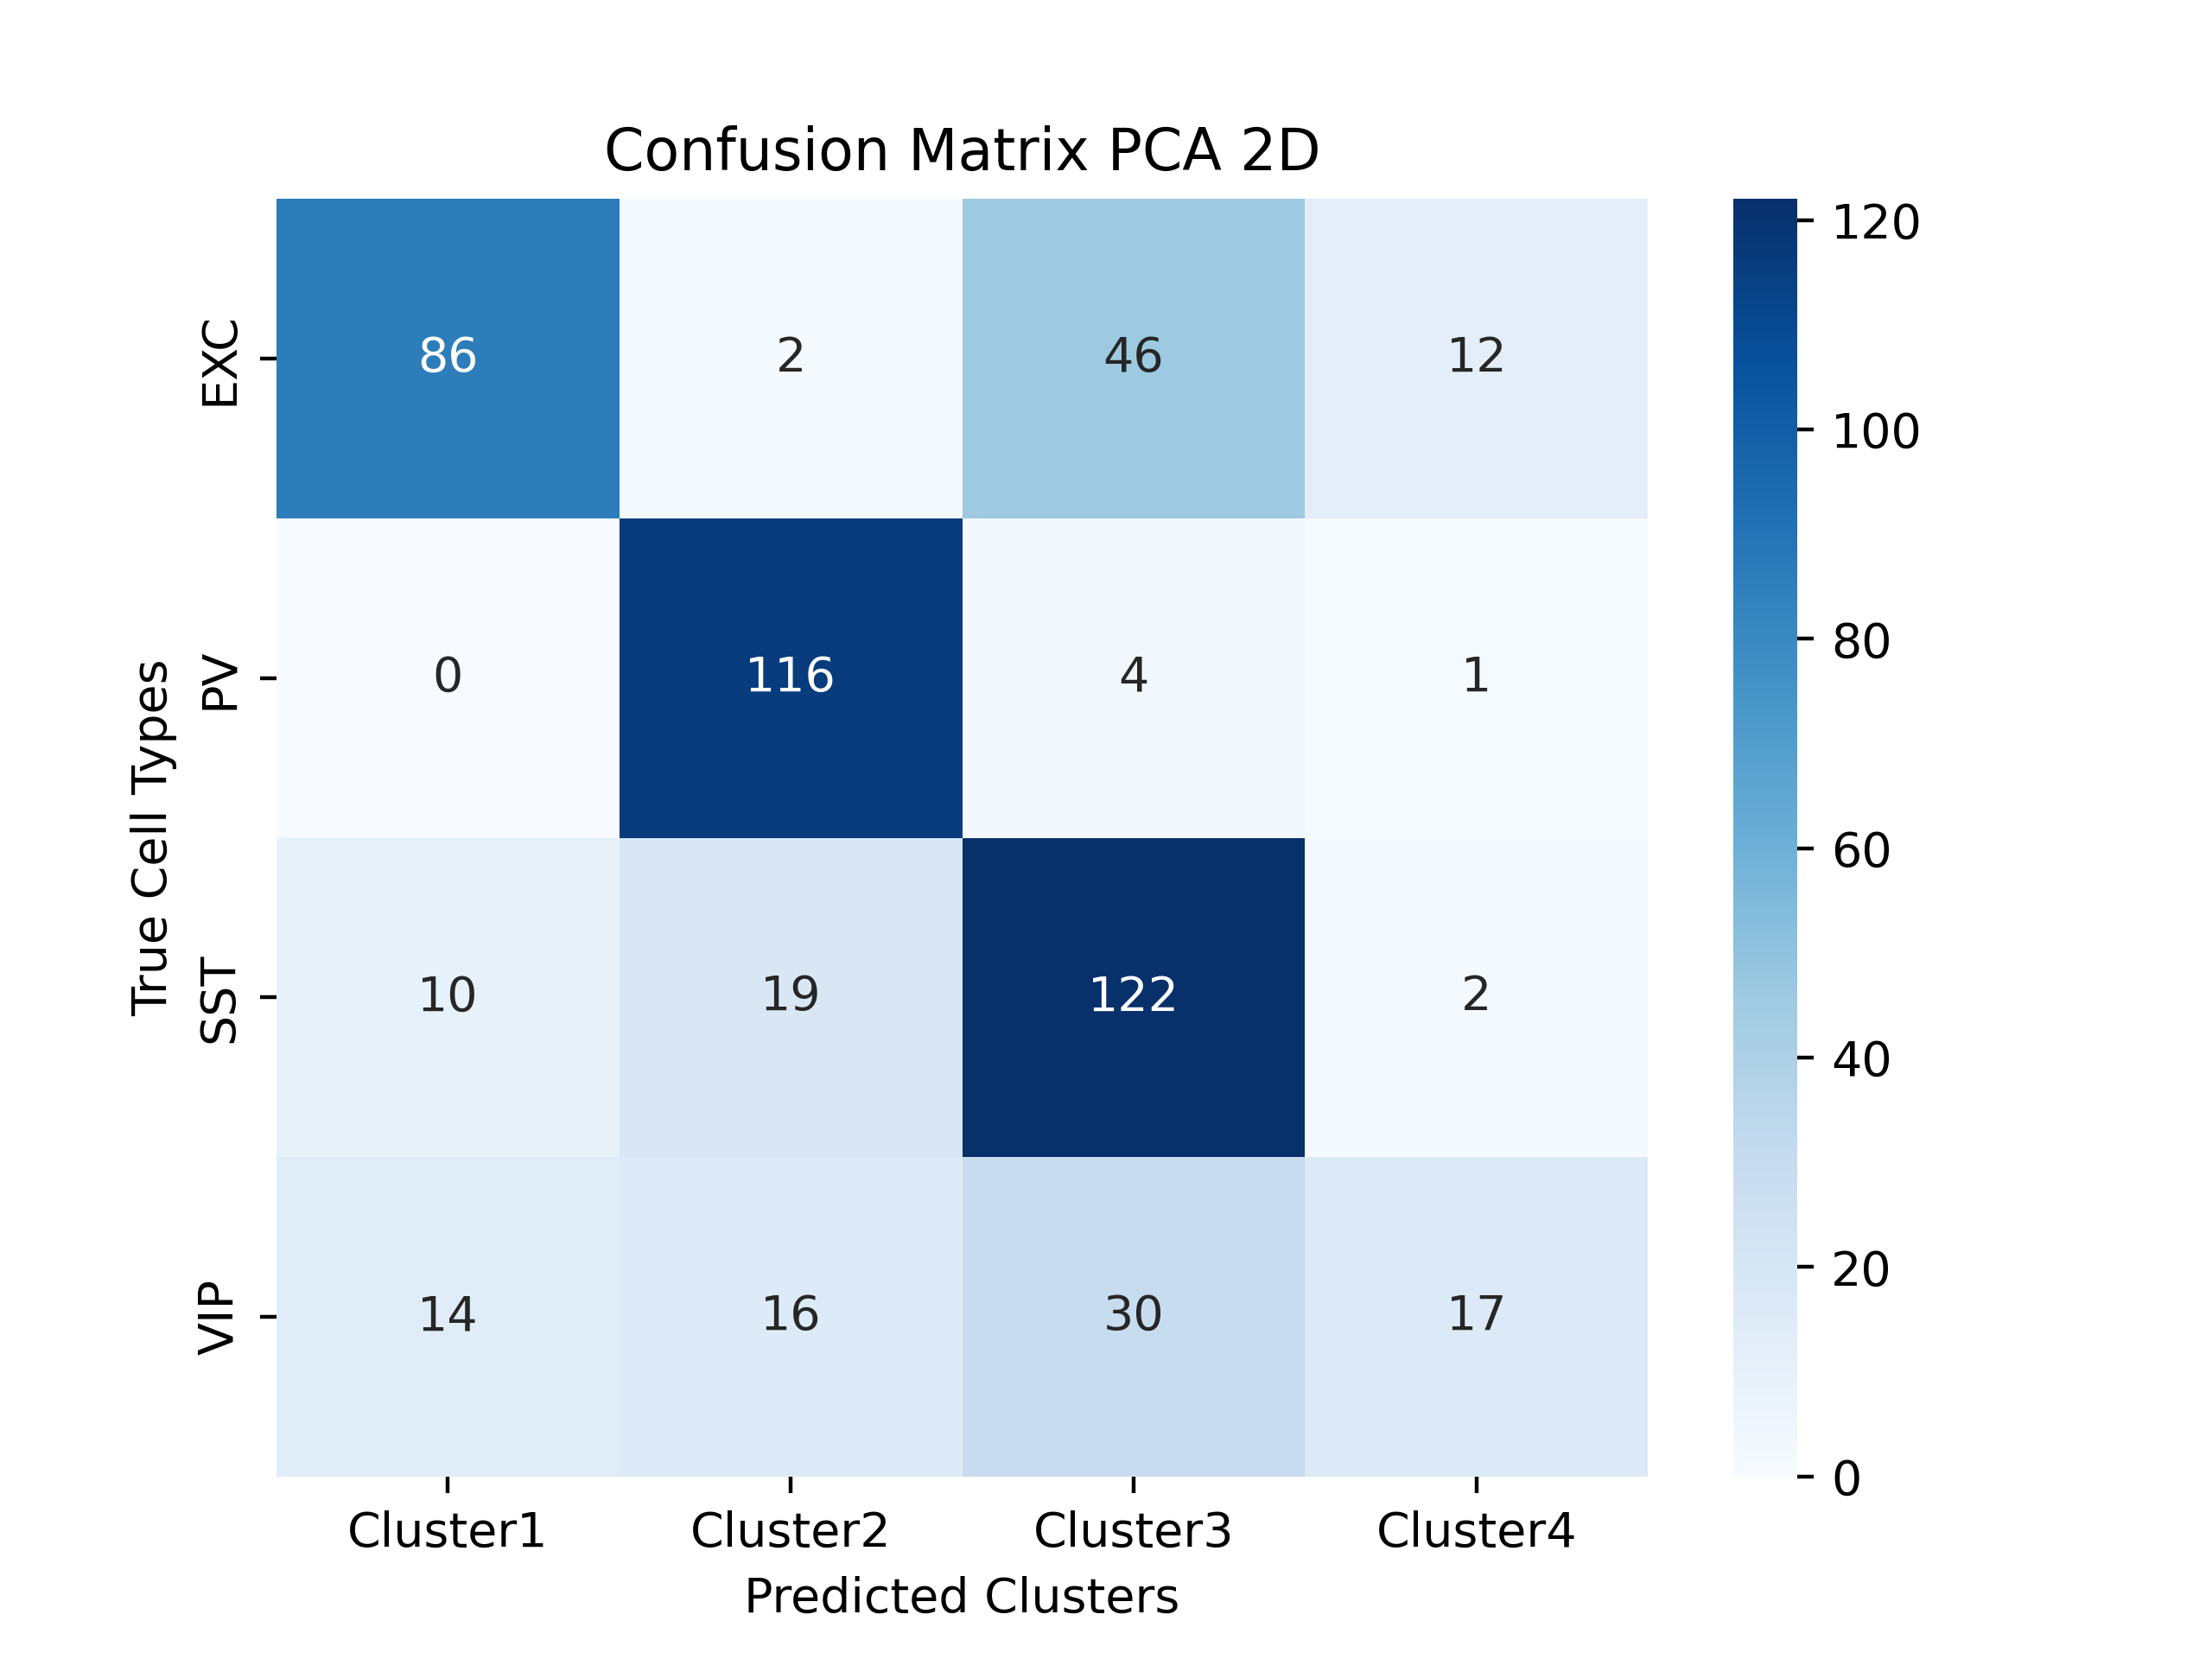
\includegraphics[width=0.5\columnwidth]{figures/Confusion Matrix PCA 2D.png}
%   \caption{}
%   \label{fig:cfm_pca2D_wrapped}
% \end{wrapfigure}


% Example on how to add sub-captions
% \begin{figure}%
%   \centering
%   \subfloat[Confusion Matrix PCA 2D]{{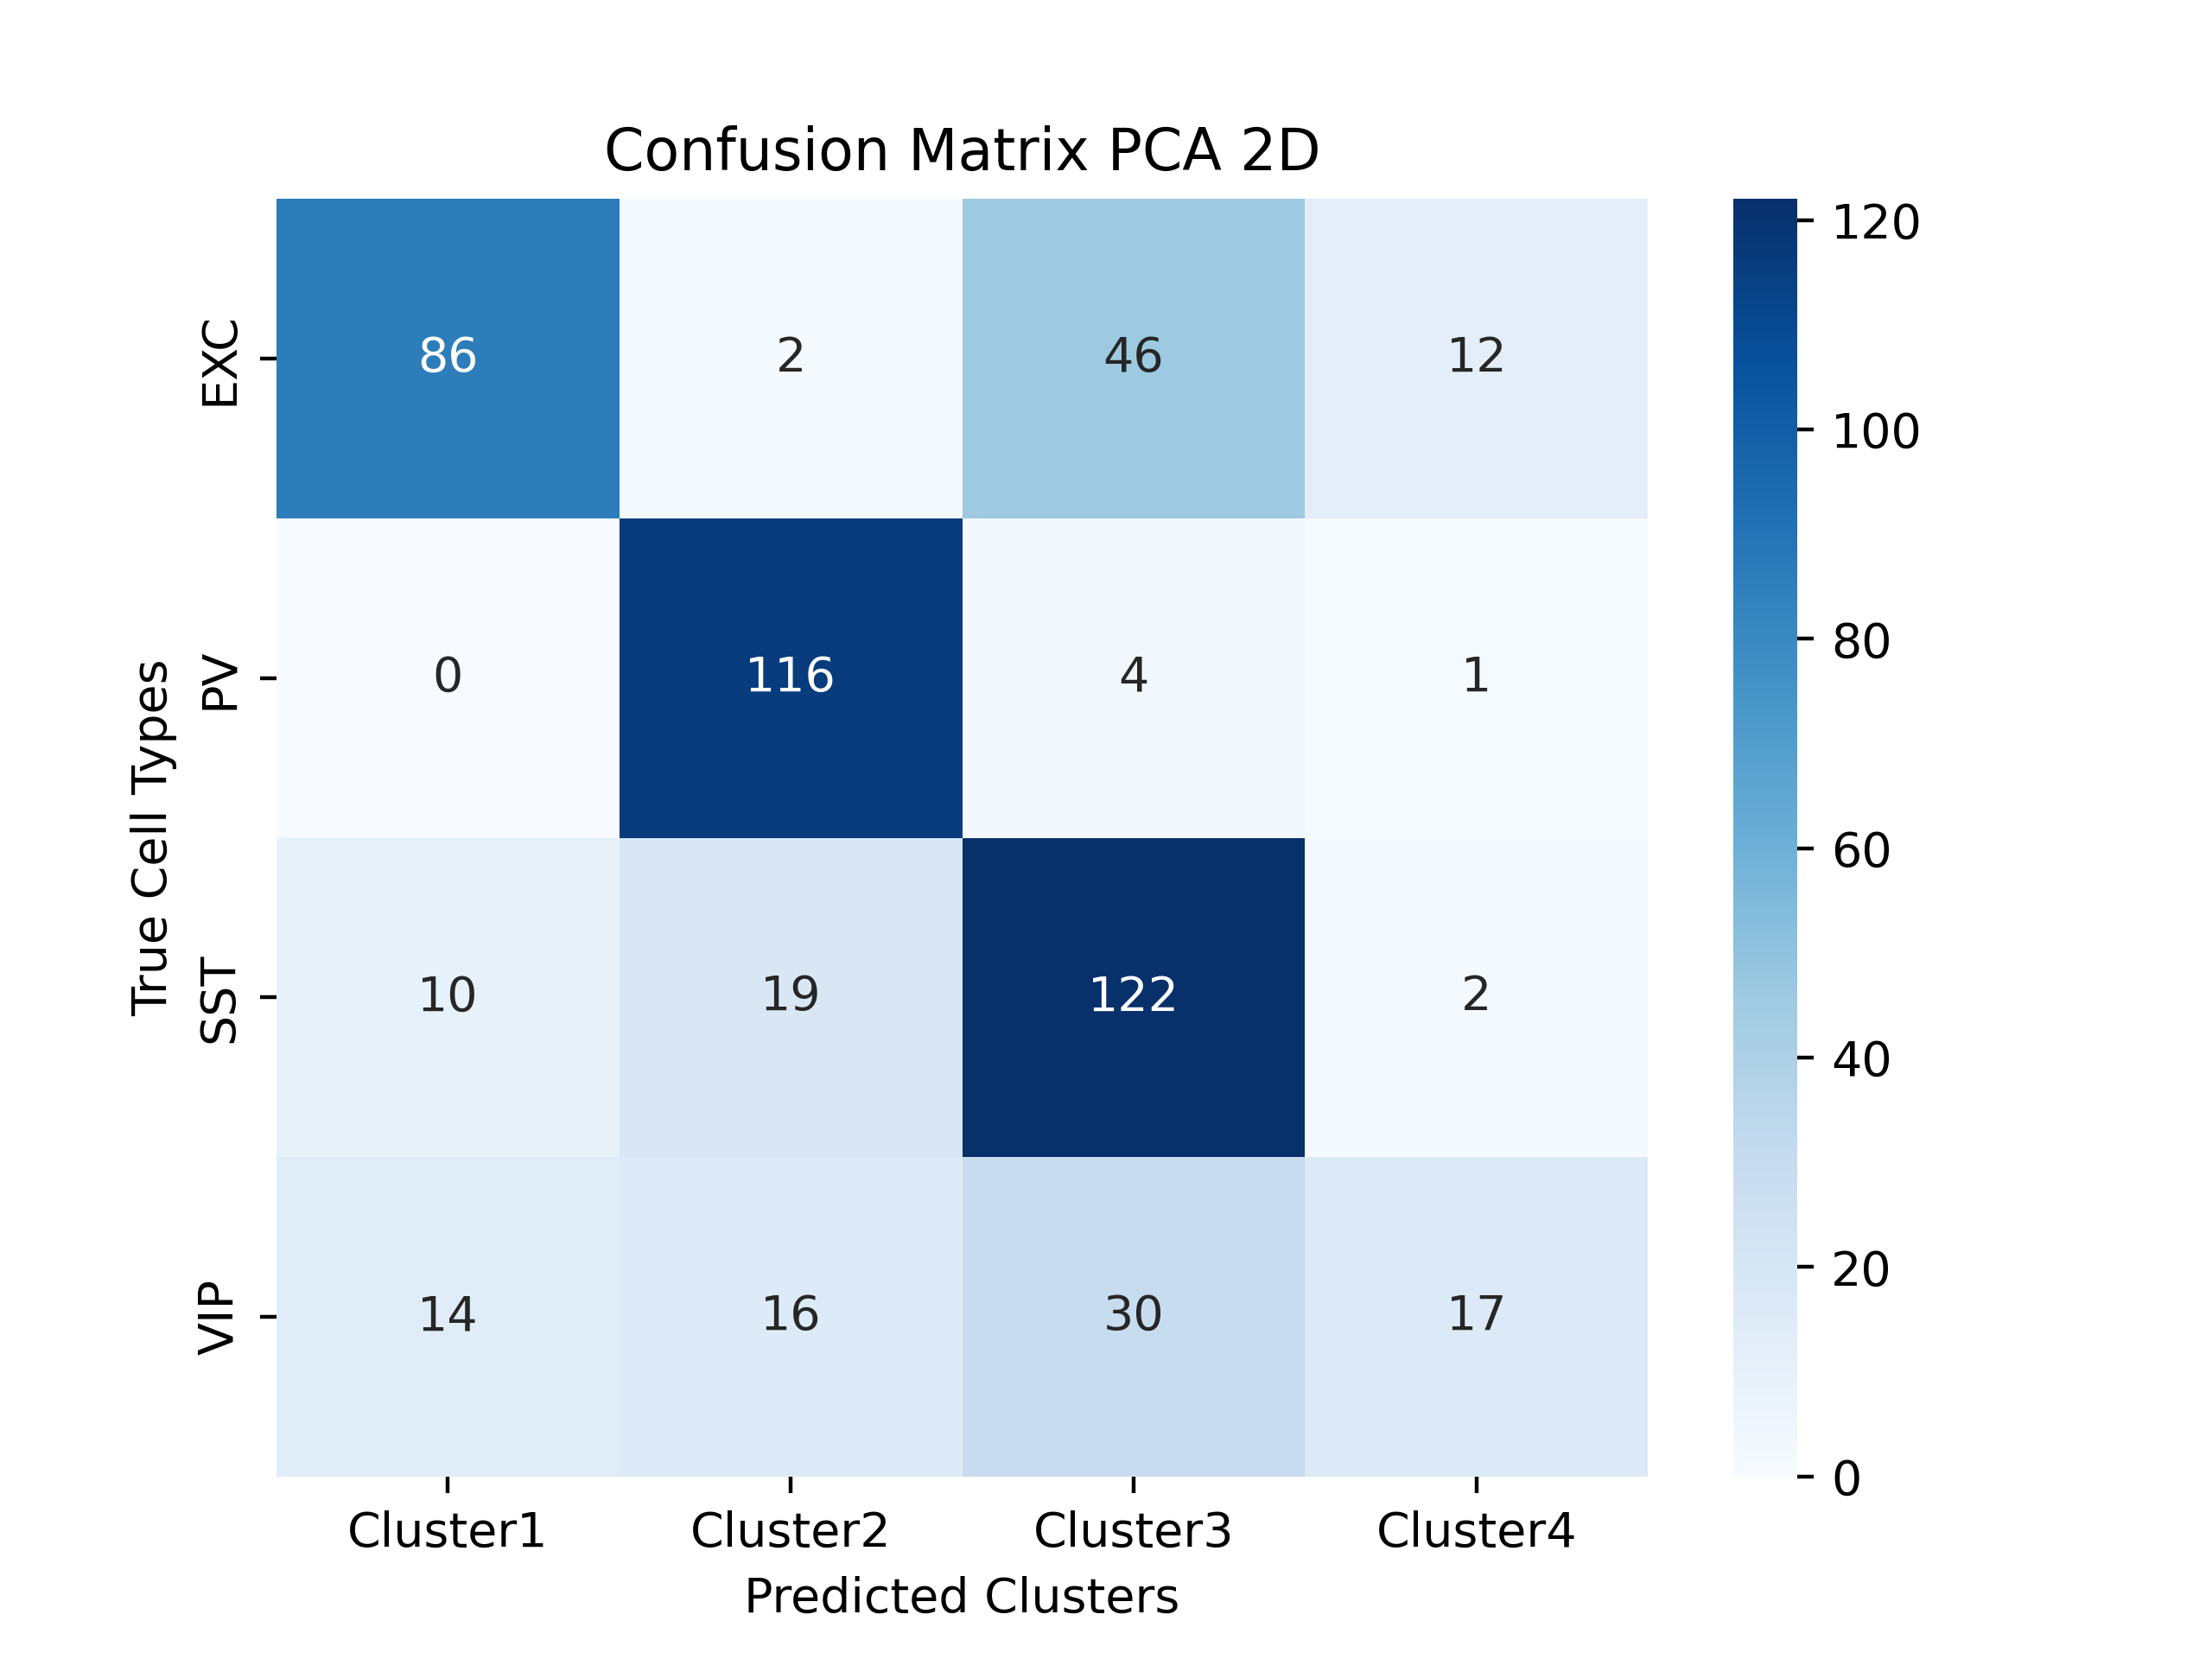
\includegraphics[width=4cm]{figures/Confusion Matrix PCA 2D.png} }}%
%   % \qquad
%   \subfloat[Confusion Matrix PCA 3D]{{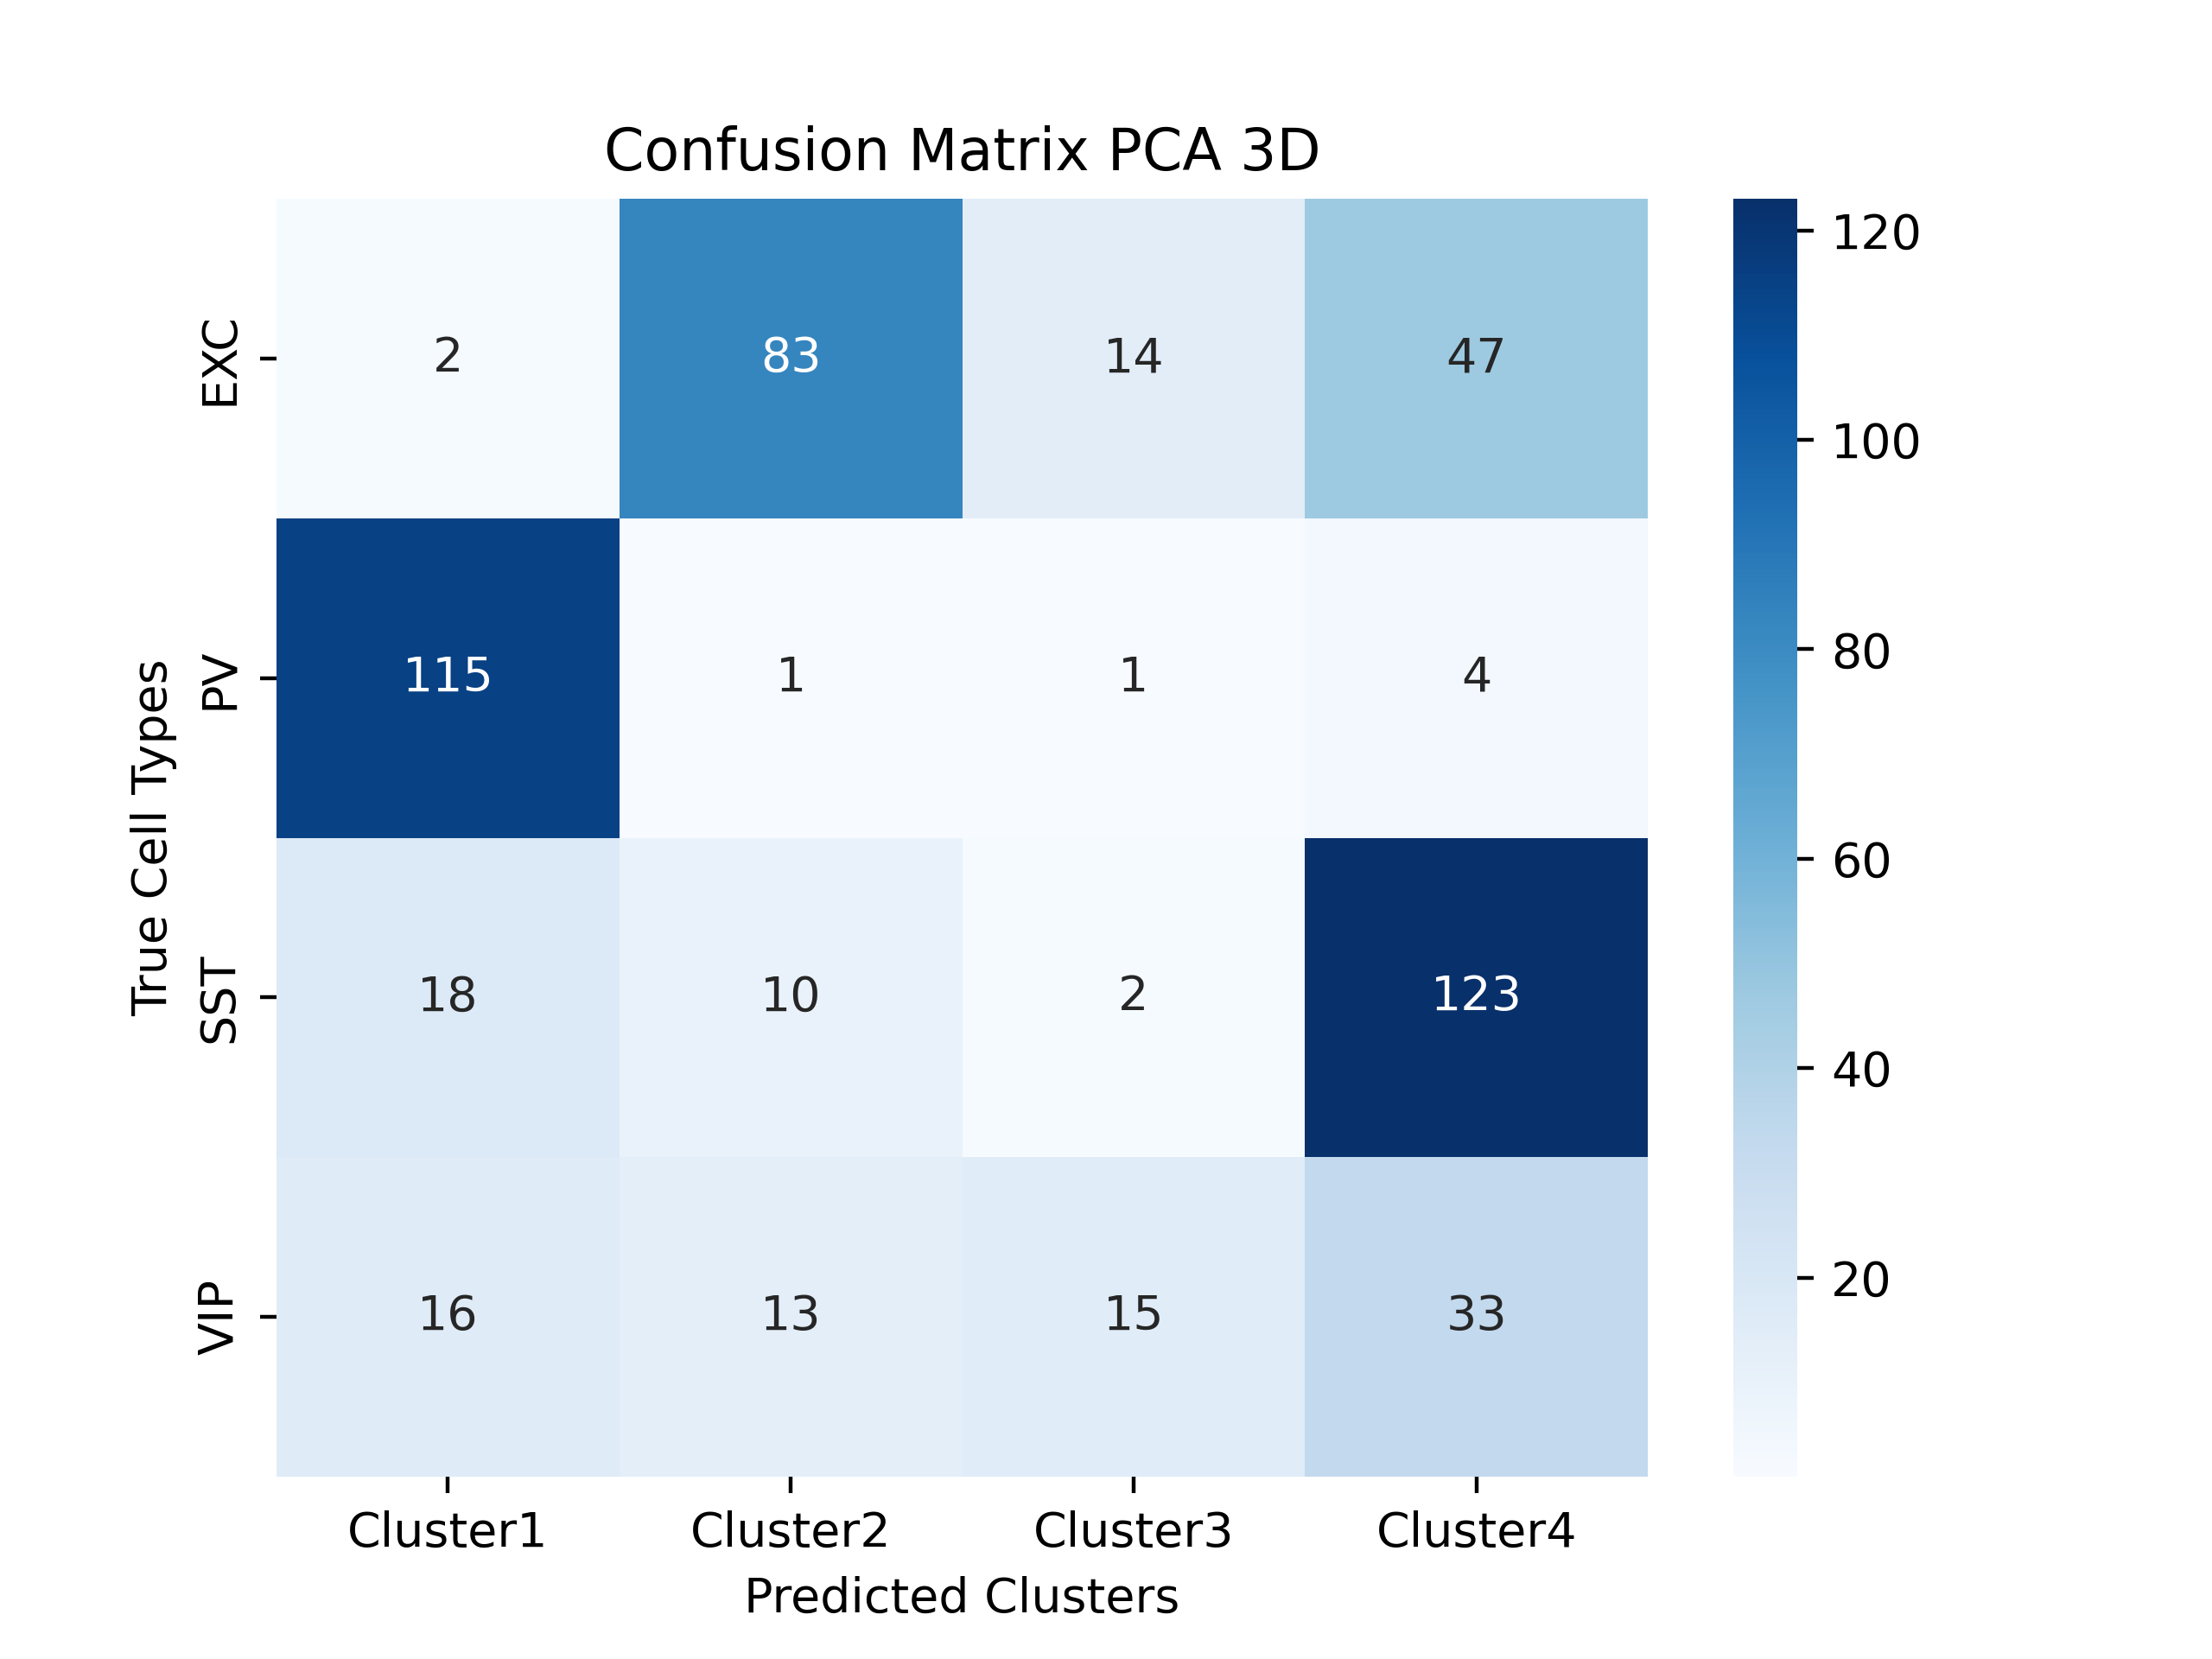
\includegraphics[width=4cm]{figures/Confusion Matrix PCA 3D.png} }}%
%   \caption{2 Figures side by side}%
%   \label{fig:example}
% \end{figure}


\begin{abstract}
  This study explores the use of interpretable Machine Learning tools in order to try and identify what are the most distinct characteristics of known cortical neuron types. As such we analyzed the contribution and importance of different features, on supervised learning classification algorithms. In addition, dimensionality reduction and unsupervised learning techniques were employed to enrich our analysis. 
  Section II is dedicated to answering the demanded questions.
\end{abstract}

%-----------------------------------------------------

\section{Introduction}

% Explain in a few lines what is the question you want to address, what is the rational, and what is your hypothesis? % TODO

Neural dynamics and cellular behavior within the brain presents an ongoing challenge for understanding its complexities. In this pursuit, the present study delves into the classification of distinct neuronal cell types based on a set of carefully selected features derived from electrophysiological data. Focusing on ``free whisking" sweeps, this study employs a range of machine learning techniques, both supervised and unsupervised, to unravel patterns and relationships within the dataset. The chosen predictors, spanning from firing rates to spectral domain information, aim to capture nuanced aspects of neuronal activity. Through rigorous model testing, hyperparameter optimization, and dimensionality reduction, the study seeks not only to classify cell accurately types but also to uncover the underlying features pivotal in this classification.

%-----------------------------------------------------

\section{Answers to Questions}

All relevant figures to answer questions, can be visualized in Annex.

\subsubsection{Impact of AP Threshold, Mean Vm, and SD of Vm on the Mean Firing Rate}

The mean firing rate of neurons is intricately linked to properties such as the action potential (AP) threshold, mean membrane potential (Vm), and standard deviation (SD) of Vm.
The firing rate exhibits a significant correlation with the mean Vm (Fig. \ref{fig:3_8} bottom left), and to a lesser extent, with the standard deviation of Vm (Fig. \ref{fig:3_8} bottom right). 
A higher mean Vm generally corresponds to a lower firing rate, which is consistent with established principles. Intuitively, the lower the AP threshold, the higher the firing rate, however, this relationship does not hold uniformly across all cell classes as no clear correlation was observed with the AP threshold (Fig. \ref{fig:3_8} top right).
% Additionally, for all cell classes, one can observe a significant linear correlation between the change in firing rate and the change in Vm at whisking onset (Fig. \ref{fig:deltaFR_vs_deltaVm}).

\subsubsection{Specificities of each cortical neuron class allowing to distinguish excitatory vs inhibitory neurons (Fig. \ref{fig:1_2_4_5_7})}

\begin{itemize}
  \item Excitatory Neurons: Excitatory neurons exhibit overall low action potential firing rates and hyperpolarized membrane potential.
  
  \item PV-expressing GABAergic Neurons: PV neurons fire at higher rates than other classes and have short AP durations.
  
  \item VIP-expressing GABAergic Neurons: VIP neurons, have longer AP durations than other inhibitory neurons.
  
  \item SST-expressing GABAergic Neurons: SST neurons, relatively low FR compared to other inhibitory neurons, a much smaller FFT amplitude and a much smaller SD in their membrane potential.
\end{itemize}


\subsubsection{Whisking versus Active-Contact Onset Time}

\subsubsection*{Whisking Onset Time}

\begin{itemize}
    \item Excitatory Neurons: Excitatory neurons depolarize at whisking onset, with a brief transient hyperpolarization shortly after. Superficial neurons exhibit more depolarization compared to deeper neurons.
    
    \item PV-expressing GABAergic Neurons: PV neurons depolarize at whisking onset, with a more prominent increase in firing rate in deeper neurons.
    
    \item VIP-expressing GABAergic Neurons: VIP neurons depolarize at whisking onset, with late excitation during whisking. They are more depolarized compared to quiet periods, influenced by nicotinic input and glutamatergic input from other cortical regions.
    
    \item SST-expressing GABAergic Neurons: On average, SST neurons hyperpolarize at whisking onset. Superficial SST neurons may show a prominent hyperpolarization.
\end{itemize}

\subsubsection*{Active-Contact Onset Time}

\begin{itemize}
    \item Excitatory Neurons: Excitatory neurons show robust depolarization with a small increase in firing rate during active touch. There's a frequency-dependent suppression of touch-evoked responses at short intercontact intervals.
    
    \item PV-expressing GABAergic Neurons: PV neurons exhibit large and fast depolarization during active touch. Touch-evoked responses are suppressed at short intercontact intervals, but with a reliable peak Vm.
    
    \item VIP-expressing GABAergic Neurons: VIP neurons depolarize and increase firing rate during active touch. They show late excitation during active touch, consistent with a delayed response.
    
    \item SST-expressing GABAergic Neurons: SST neurons display relatively weak active touch responses, with a unique response to intercontact intervals, showing a small hyperpolarization at long intervals and excitatory PSP response at short intervals.
\end{itemize}

Now we transition to the actual study.

%-----------------------------------------------------

\section{Methods}

\subsection{Data Preprocessing}
\subsubsection{Predictors}

We decided to focus only on “free whisking” sweeps, which amounted to 497 different samples.
From these sweeps we decided to use as predictors the calculated firing rate (\textit{firing\_rate}), action potential (AP) threshold and duration (\textit{ap\_threshold} and \textit{ap\_duration}), the mean and the standard deviation of the membrane potential (\textit{mean\_vm} and \textit{std\_vm}), and spectral domain information in the form of the lowest and the highest Fourier amplitudes (\textit{fft\_low} and \textit{fft\_high}).
Whenever a sweep did not have an AP, we replaced both AP duration and threshold by a value of 0. In hindsight this is biologically nonsensical.
These seven features created a data matrix $X_1 \in \mathbb{R}^{497\times7}$ to be paired with the response variable $y \in \mathbb{R}^{497\times1}$ corresponding to each cell class.

\subsubsection{Additional Extracted features}
In addition to the 7 features mentioned above, the 13 features described in Table-\ref{tab:variables} were extracted and added from each sweep, widening our data size $X_2 \in \mathbb{R}^{497\times20}$.
One can observe the correlation between each variable present in $X_2$, in Annex (Fig. \ref{fig:correlation}). 

\subsubsection{Standardization}
For supervised learning, the $X_2 \in \mathbb{R}^{497\times20}$ data was used. When splitting, training data was standardized, and the same transformation was applied to the test data.
For unsupervised learning the $X_1 \in \mathbb{R}^{497\times7}$ data was used. It was standardized in its entirety prior to dimensionality reduction.

\begin{table}[h!]
  \centering
  \begin{tabular}{|l|p{0.6\linewidth}|}
  \hline
  \textbf{Variable} & \textbf{Description} \\
  \hline
  \textit{ap\_amp\_mean} & Average action potential amplitude for each sweep; any missing values or NaNs were replaced with 0. \\
  \hline
  \textit{ap\_amp\_cv} & Coefficient of variation (= std / mean) of the action potential amplitudes for each sweep; any missing values or NaNs were replaced with 0. \\
  \hline
  \textit{mean\_ap\_upstroke} & Average maximal rate of increase of the membrane potential during the action potential upstroke; any missing values or NaNs were replaced with 0. \\
  \hline
  \textit{ap\_upstroke\_cv} & Coefficient of variation of the maximal rate of increase of the membrane potential during the action potential upstroke; any missing values or NaNs were replaced with 0. \\
  \hline
  \textit{mean\_ap\_downstroke} & Average maximal rate of decrease of the membrane potential during the action potential downstroke; any missing values or NaNs were replaced with 0. \\
  \hline
  \textit{ap\_downstroke\_cv} & Coefficient of variation of the maximal rate of decrease of the membrane potential during the action potential downstroke; any missing values or NaNs were replaced with 0. \\
  \hline
  \textit{isi\_mean} & Average duration between consecutive action potentials (inter-spike intervals); any missing values or NaNs were replaced with 50. \\
  \hline
  \textit{isi\_cv} & Coefficient of variation of the duration between consecutive action potentials; any missing values or NaNs were replaced with 0. \\
  \hline
  \textit{irregularity\_index} & Index indicating how regular the inter-spike intervals are, i.e., the mean of the difference between the durations of consecutive ISIs; any missing values or NaNs were replaced with 0. \\
  \hline
  \textit{adaptation\_index} & Another index indicating how regular the inter-spike intervals are; equal to the sum of the durations of consecutive ISIs divided by their difference. It is zero for a constant firing rate, negative for an increasing firing rate, and positive for a decreasing firing rate; any missing values or NaNs were replaced with 0, and very large values were capped to $10^{10}$. \\
  \hline
  \textit{nb\_bursts} & Number of bursts per sweep. Two consecutive action potentials are considered part of the same burst if the duration between them is less than 10ms; any missing values or NaNs were replaced with 0. \\
  \hline
  \textit{mean\_burst\_dur} & Mean duration of bursts; any missing values or NaNs were replaced with 0. \\
  \hline
  \textit{burst\_dur\_cv} & Coefficient of variation of the duration of bursts; any missing values or NaNs were replaced with 0. \\
  \hline
  \end{tabular}
  \caption{Description of Added Variables}
  \label{tab:variables}
\end{table}


\subsection{Supervised Learning}

\subsubsection{Models}
In this study, a range of established machine learning algorithms available in the \textit{Sci-kit Learn} library were tested. These are Logistic Regression, Random Forest, Gradient Boosting, AdaBoost, Decision Tree, Support Vector Machines, and a Gaussian Naive Bayes.
Despite their effectiveness, deep learning models were not implemented as they would be hard to interpret.

\subsubsection{Evaluation Metric}
In order to get an estimate of the performance of each model on unseen data, we opted for a stratified 5-fold Cross Validation (CV) -which retains the original distribution when splitting the data- paired with the multi-class $F1$ score as an evaluation metric. It takes into account multi-class imbalance which was prevalent in our data (much more EXC or SST cells than VIP cells).

\subsubsection{Hyperparameter Optimization (HPO)}
Hyperparameters (HP) of a model were tuned using a Bayesian optimization algorithm available in the \textit{Scikit-Optimize} library, in order to maximise the stratified 5-fold CV $F1$ score.

\subsubsection{Feature Importance}
The (HPO) models that achieved the best test score were trained on the entire data, and each individual feature importance was assessed using a metric specific to the type of classifier used. For tree-based ensemble methods (Gradient Boosting or Random Forest), the default feature importance attribute was used. It is computed as the mean and standard deviation of accumulation of the impurity decrease within each tree. For linear models utilizing weights (Linear SVC and Logistic Regression), the mean absolute weights across each class was used.

\subsubsection{Ensembling}
After having found the top models, we wanted to see whether combining their predictions would yield a higher result. As such, a final ``ensemble" voting classifier with a majority voting rule was created and evaluated.

\subsection{Unsupervised Learning}


\begin{figure*}[h!]
  \centering
  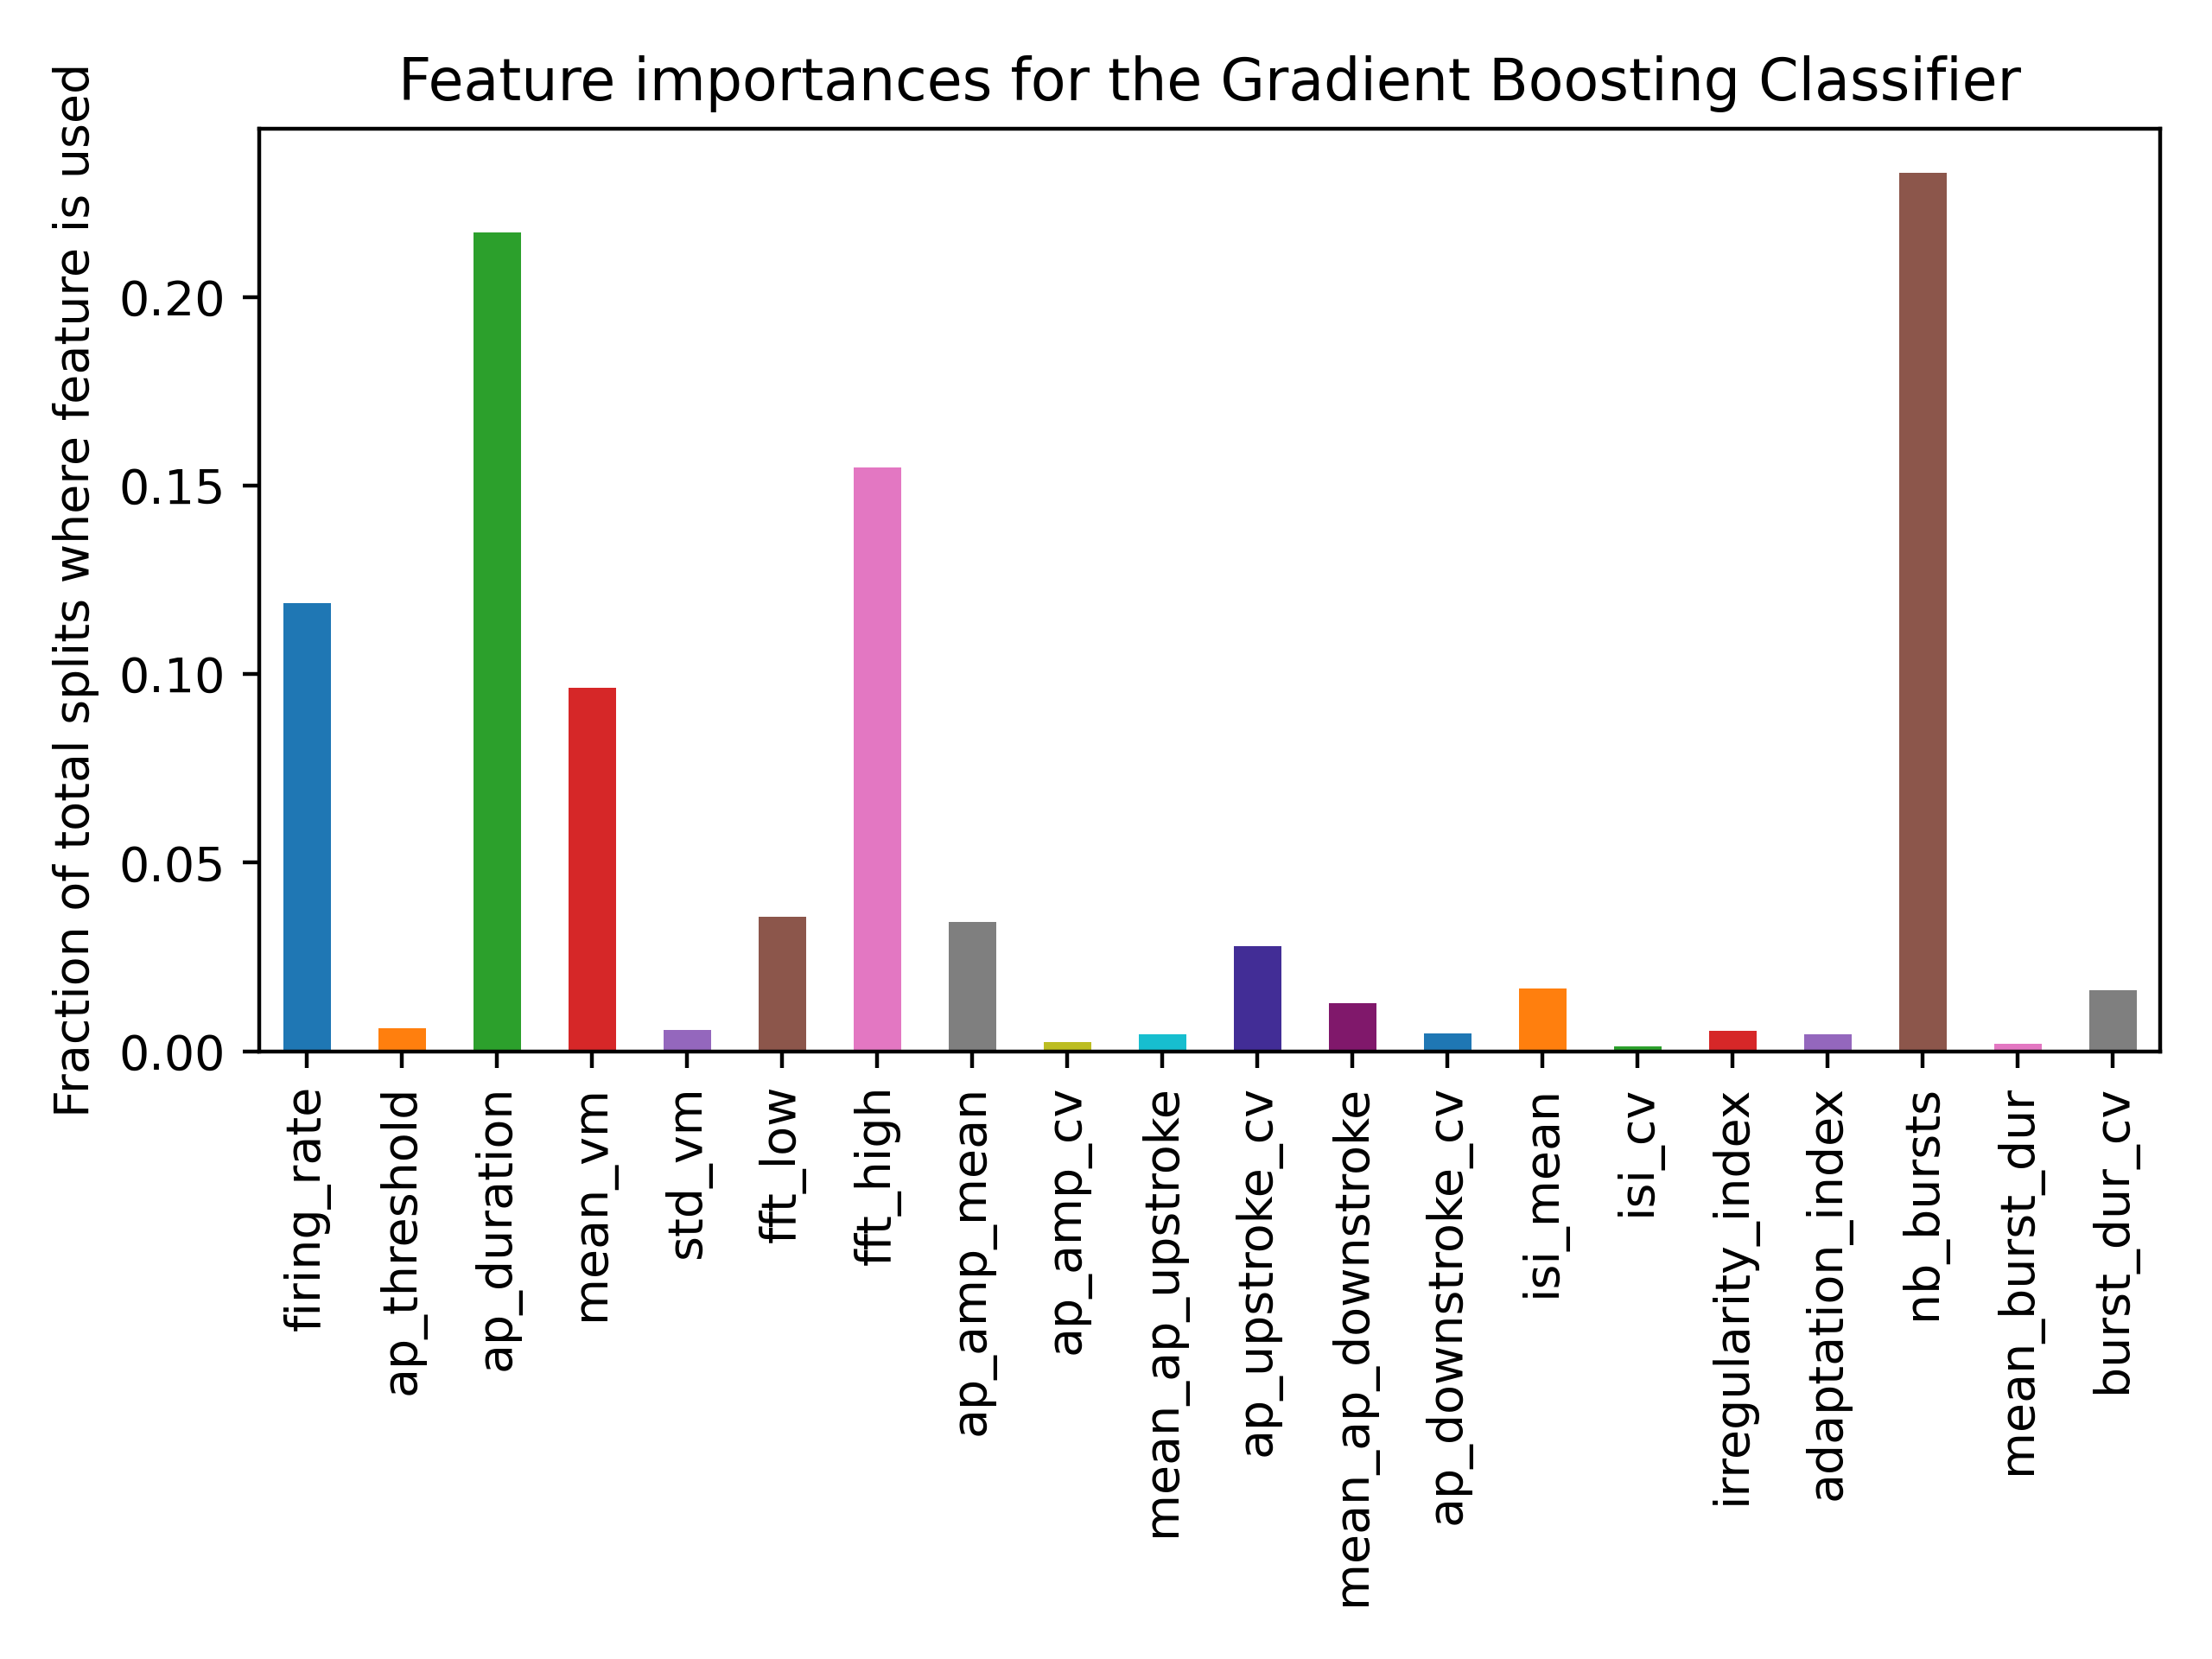
\includegraphics[width=0.9\columnwidth]{figures/feature_importance_gb.png}
  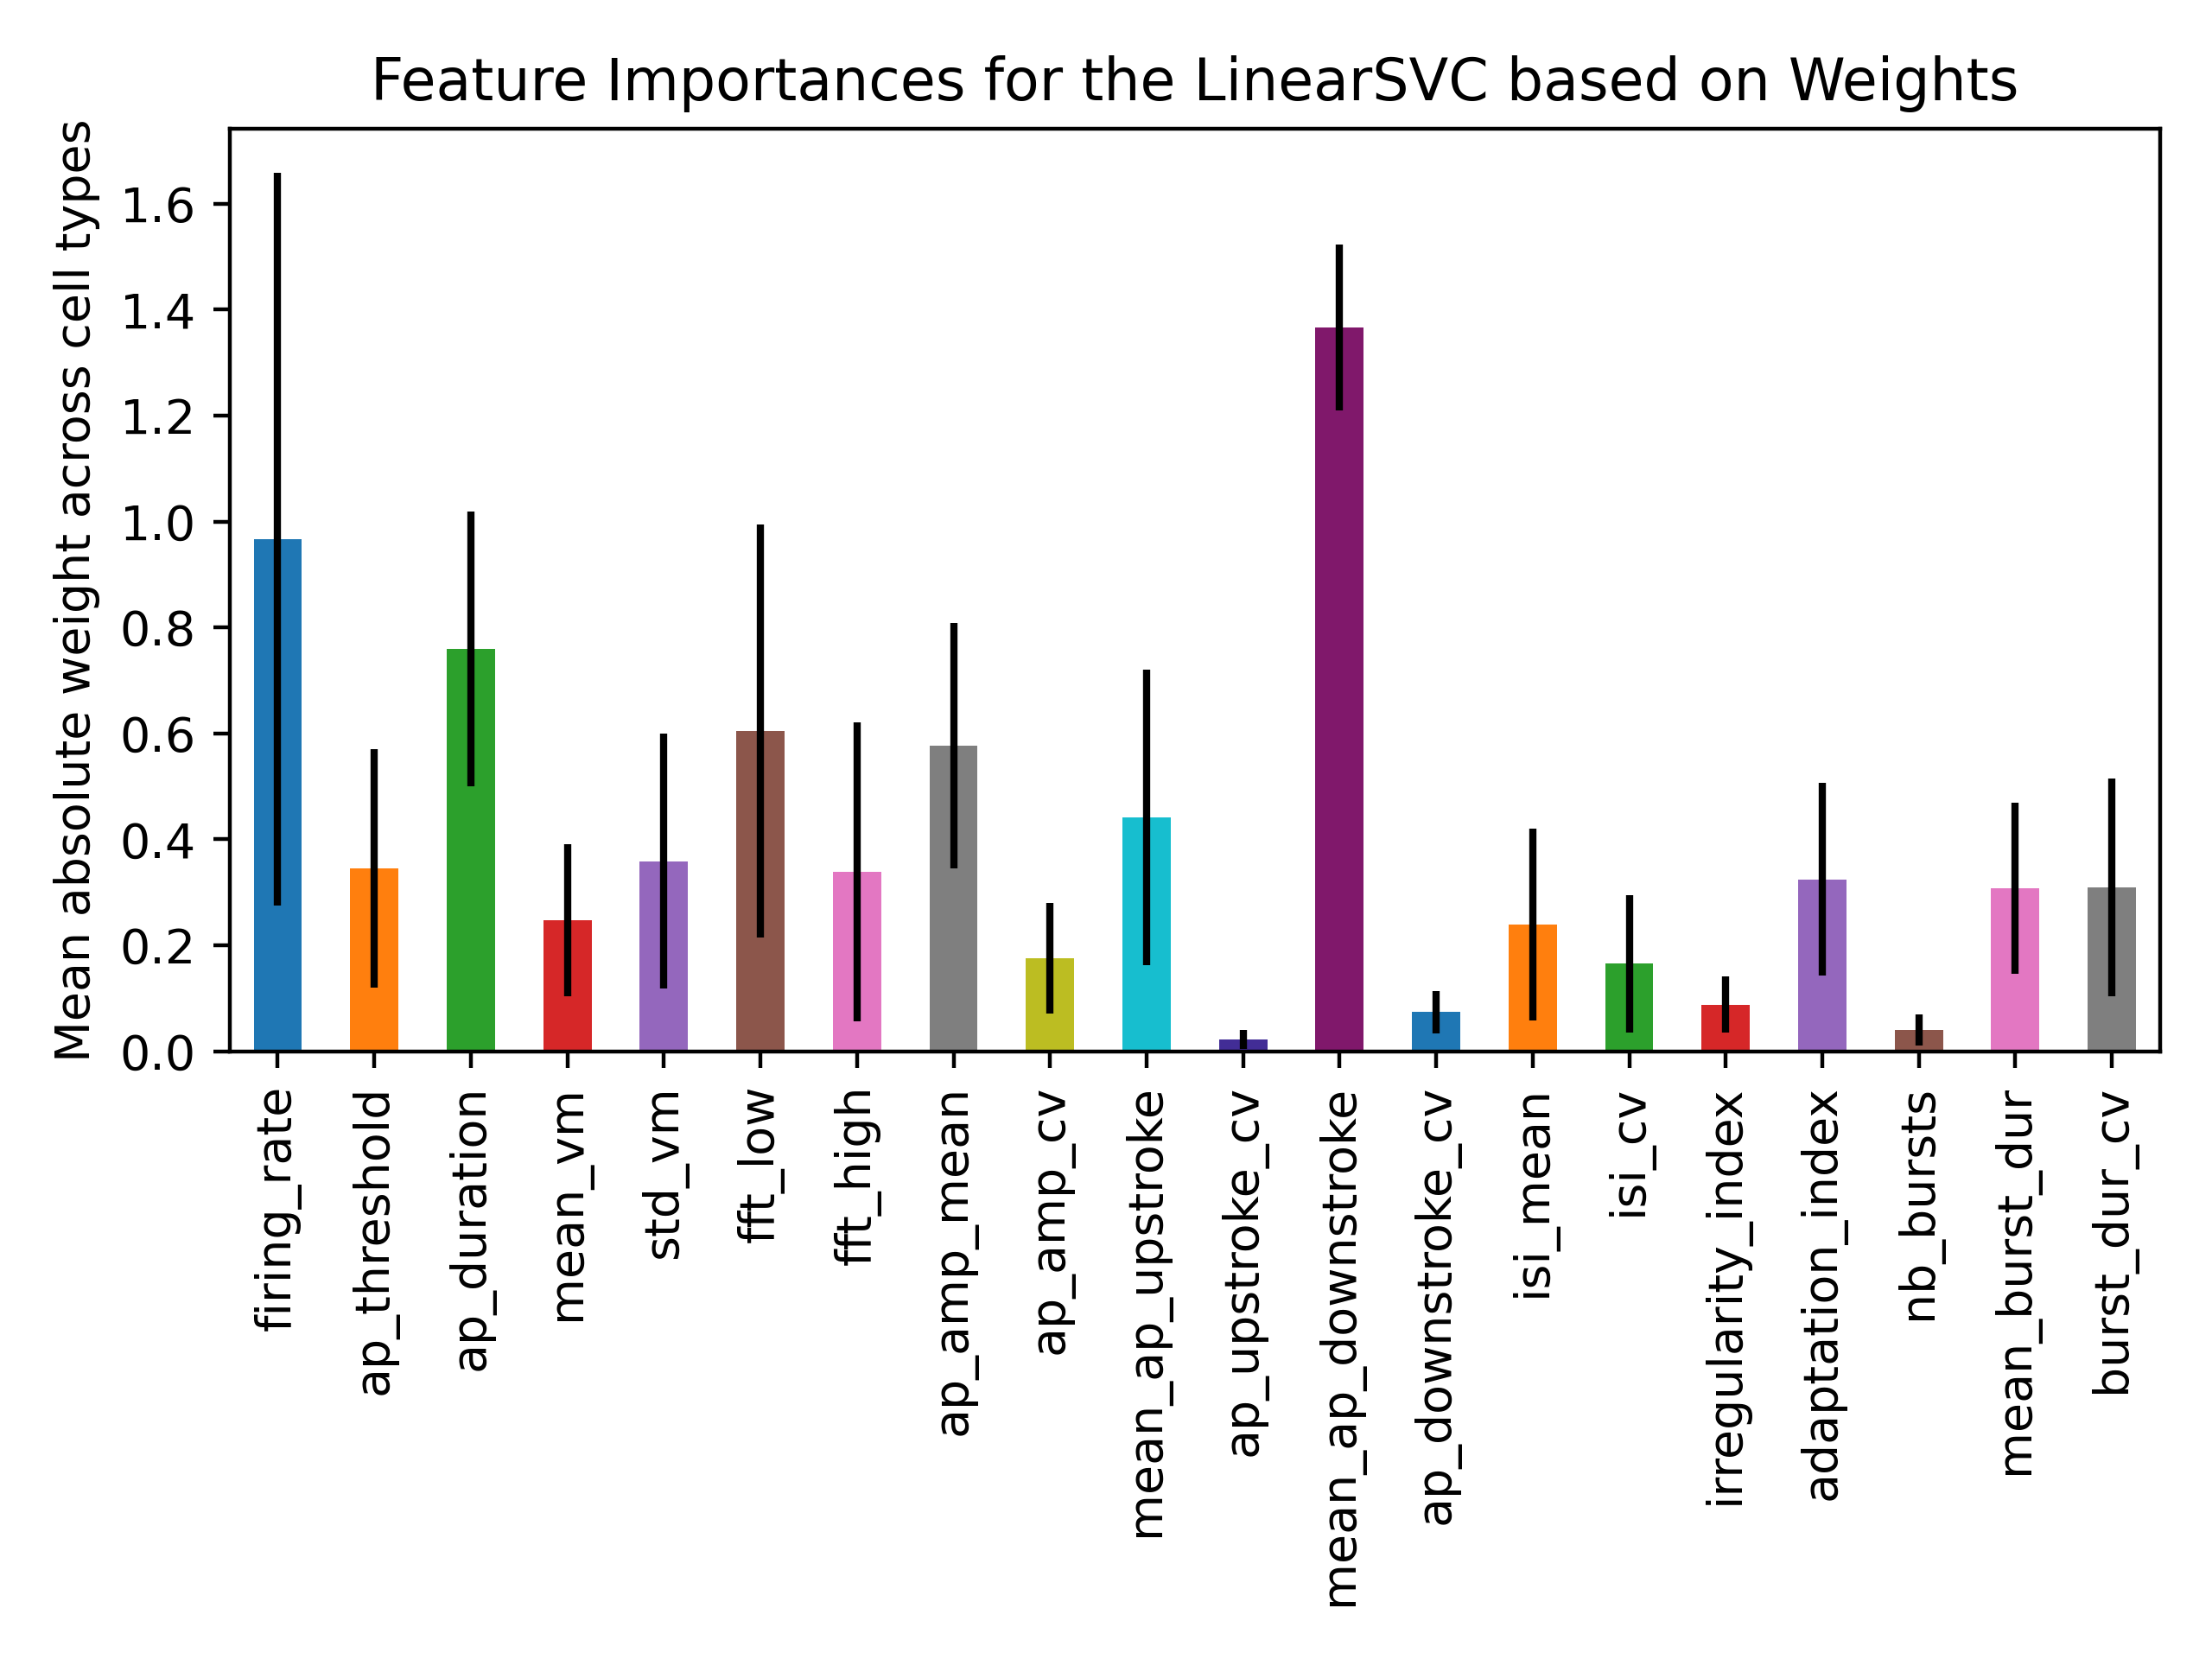
\includegraphics[width=0.9\columnwidth]{figures/feature_importance_linearsvc.png}
  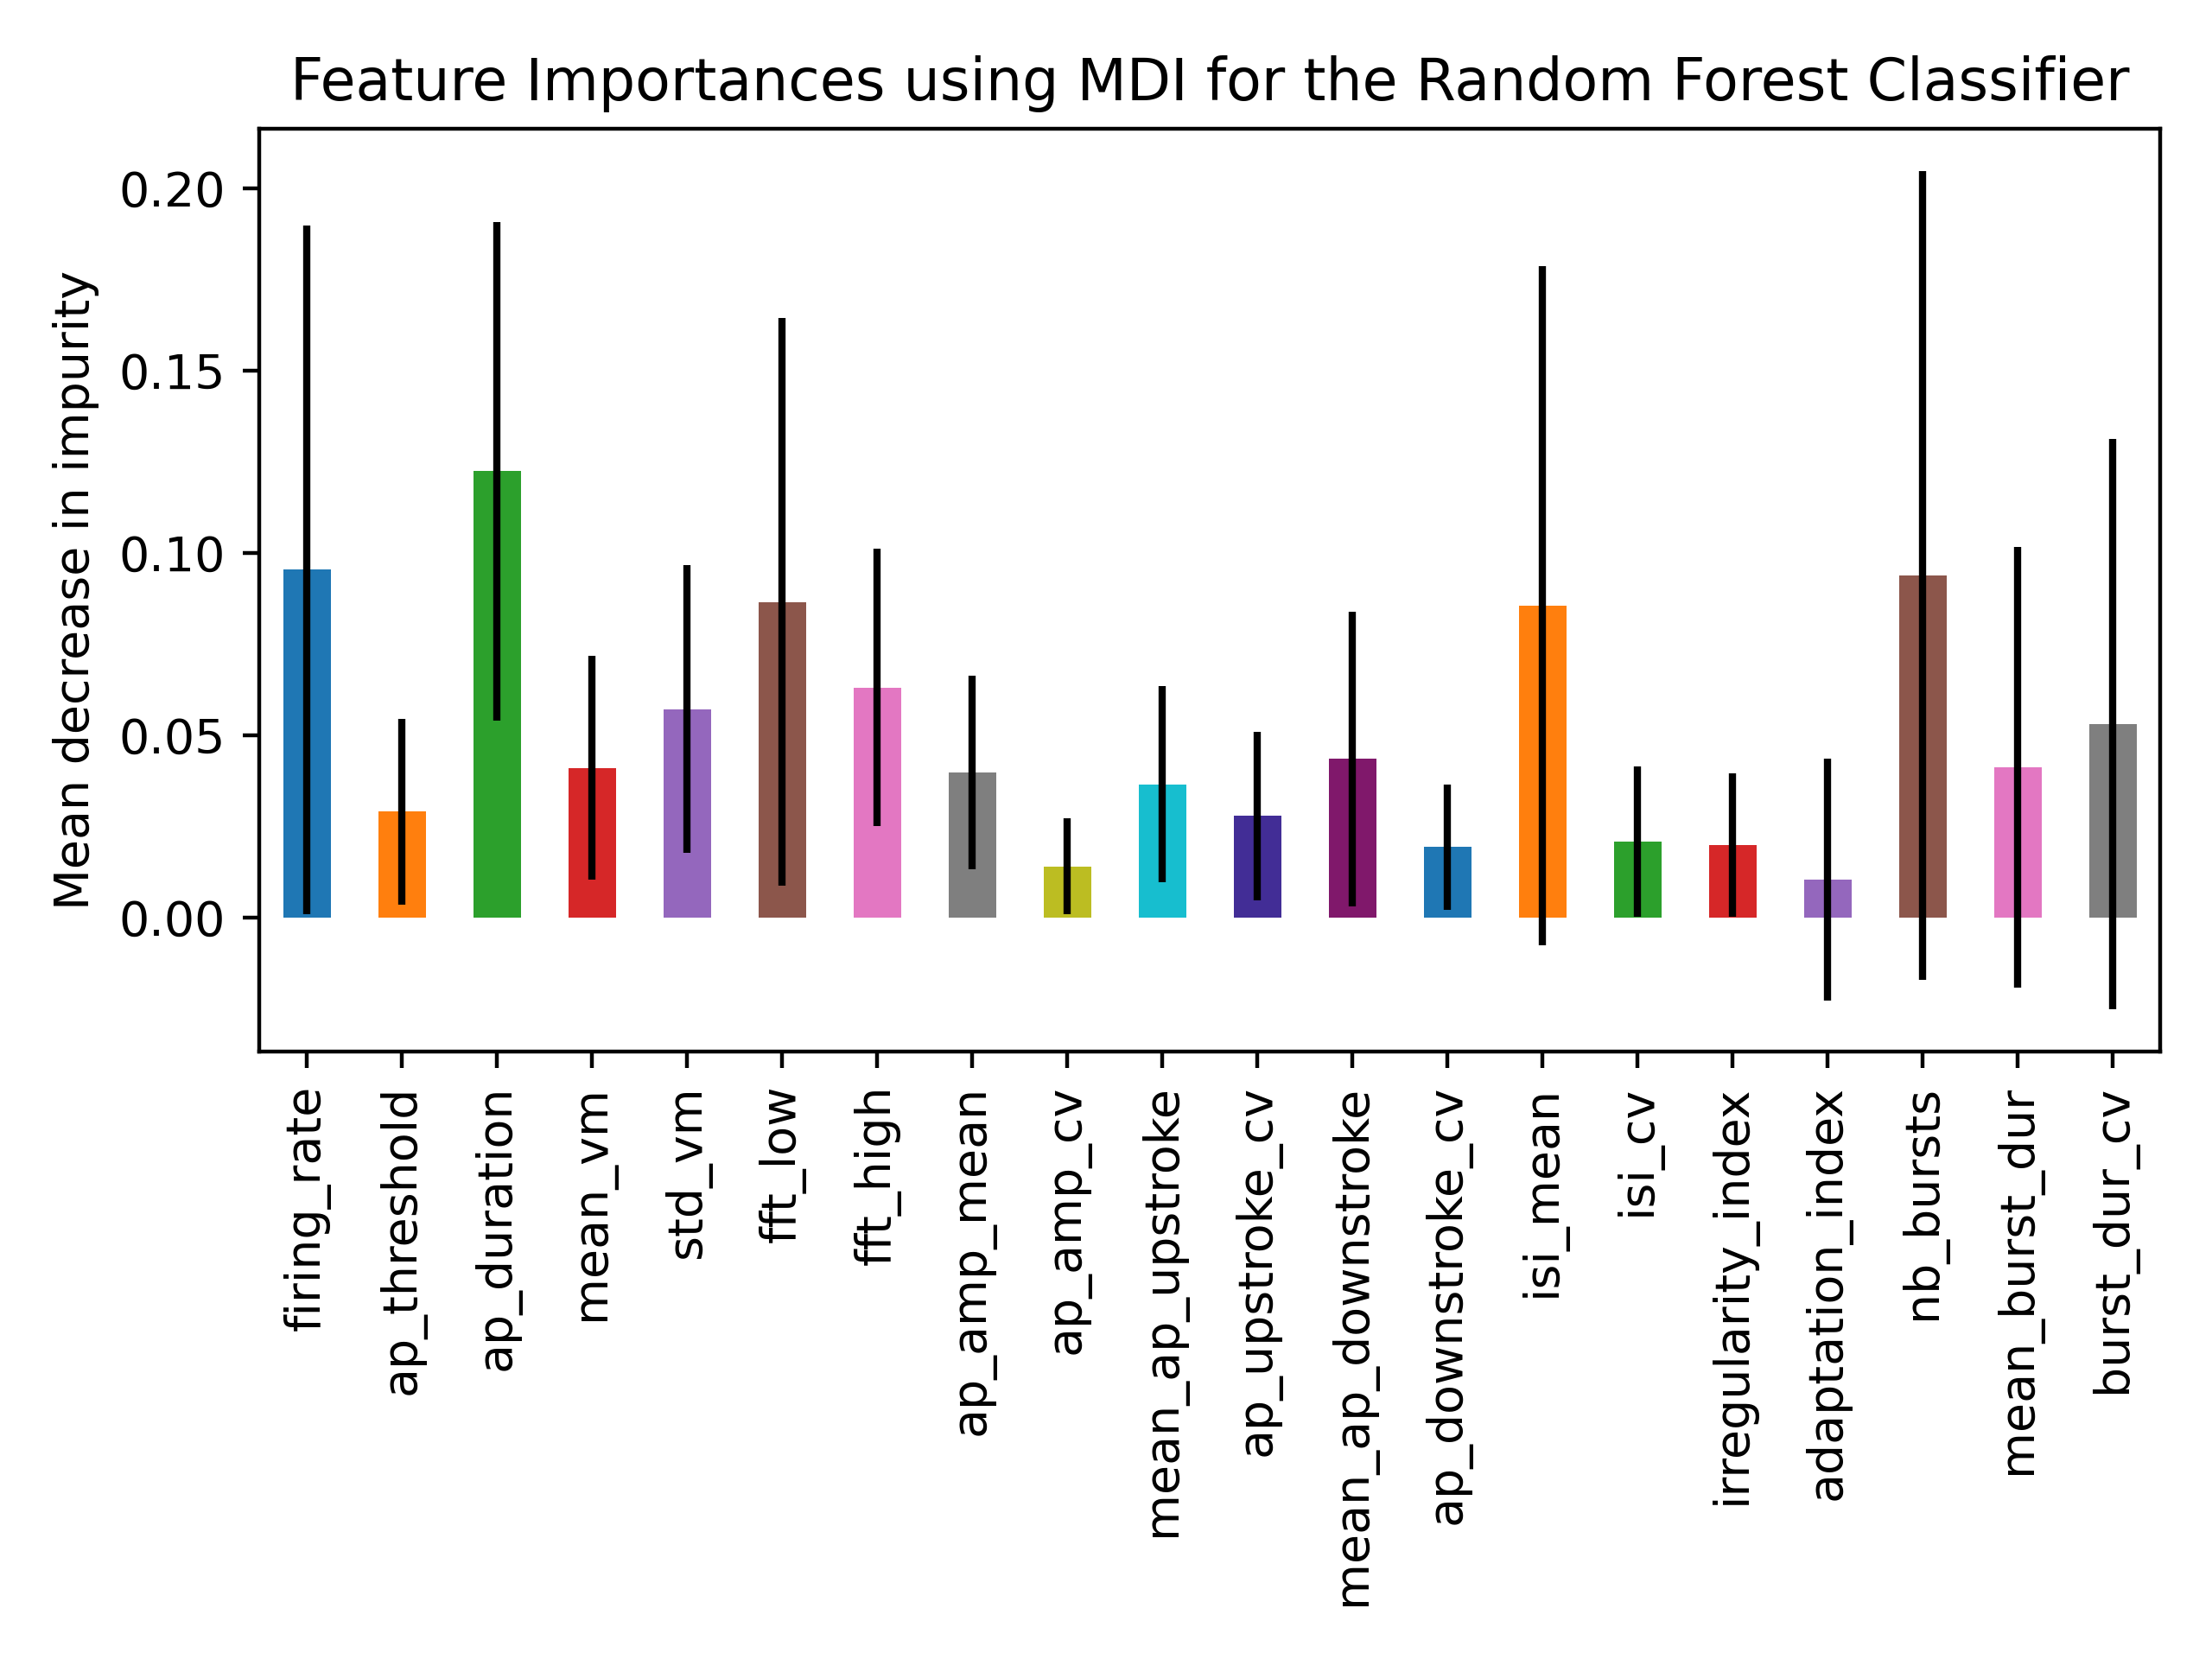
\includegraphics[width=0.9\columnwidth]{figures/feature_importance_randomforest.png}
  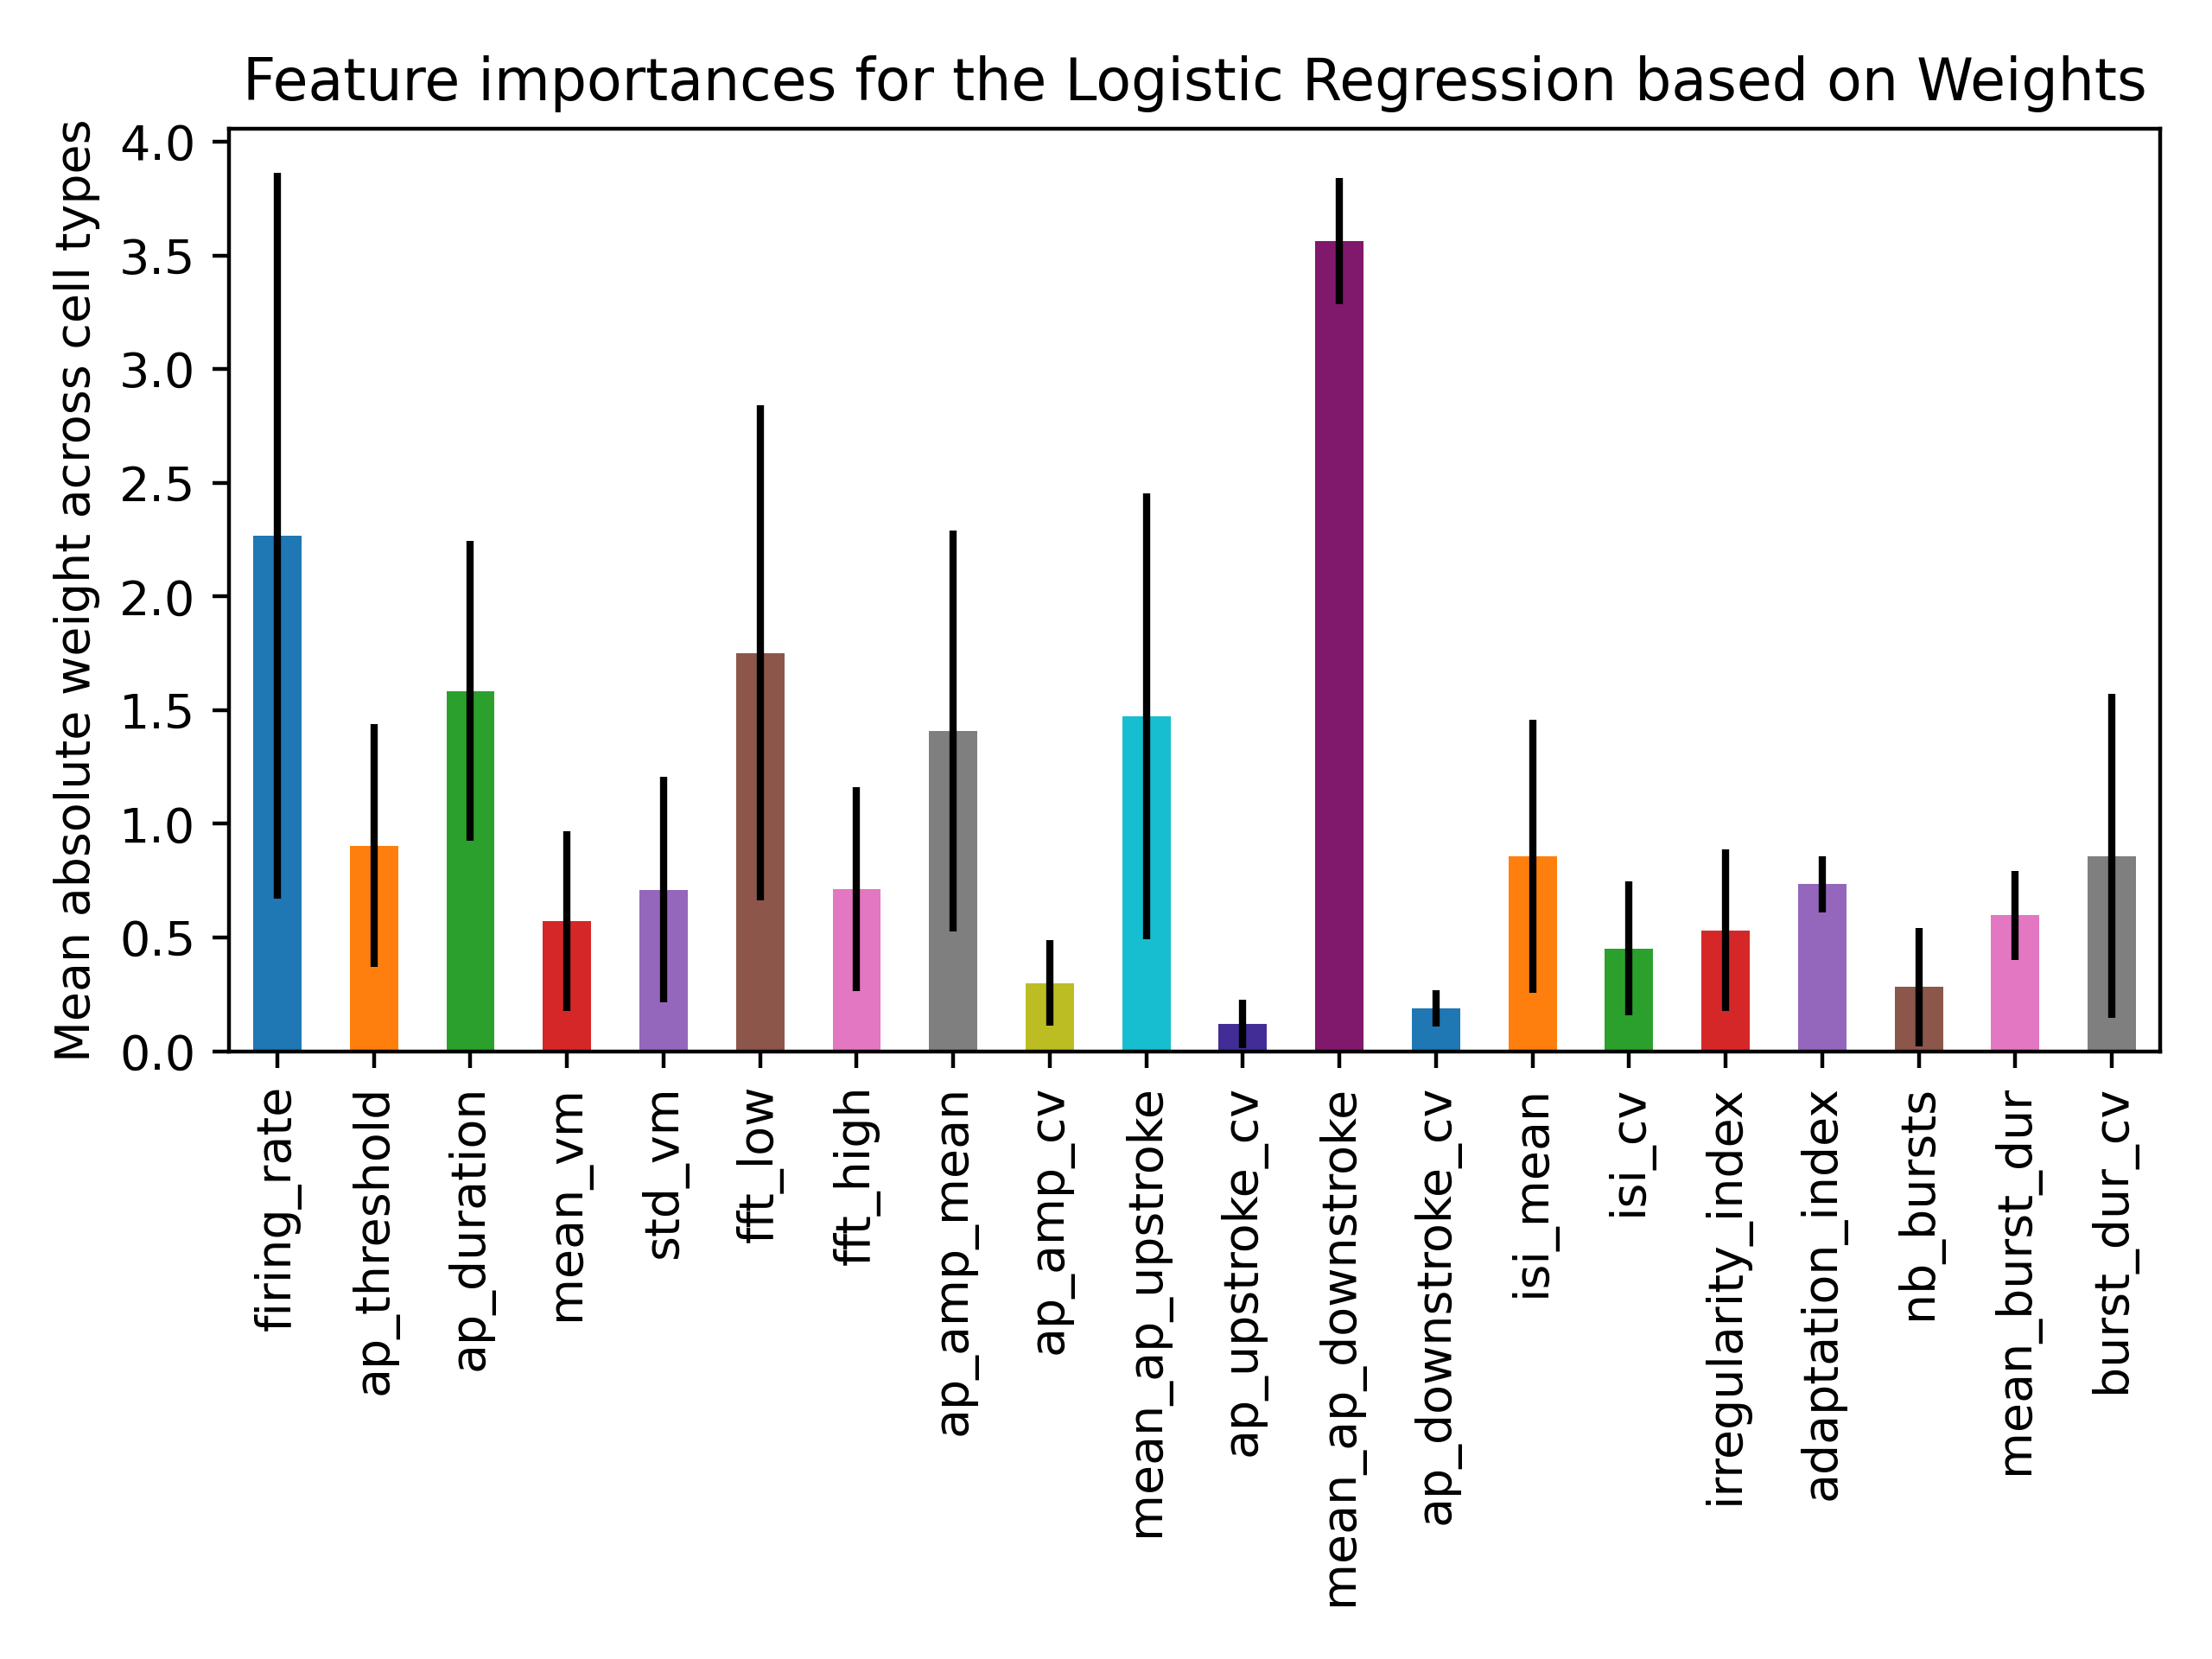
\includegraphics[width=0.9\columnwidth]{figures/feature_importance_lr.png}
  \caption{Feature importance for the top 4 best classifiers. Left column are tree-based ensembles and right column are linear models}%
  \label{fig:feature_importances}
\end{figure*}


\begin{figure*}[h!]%
  \centering
  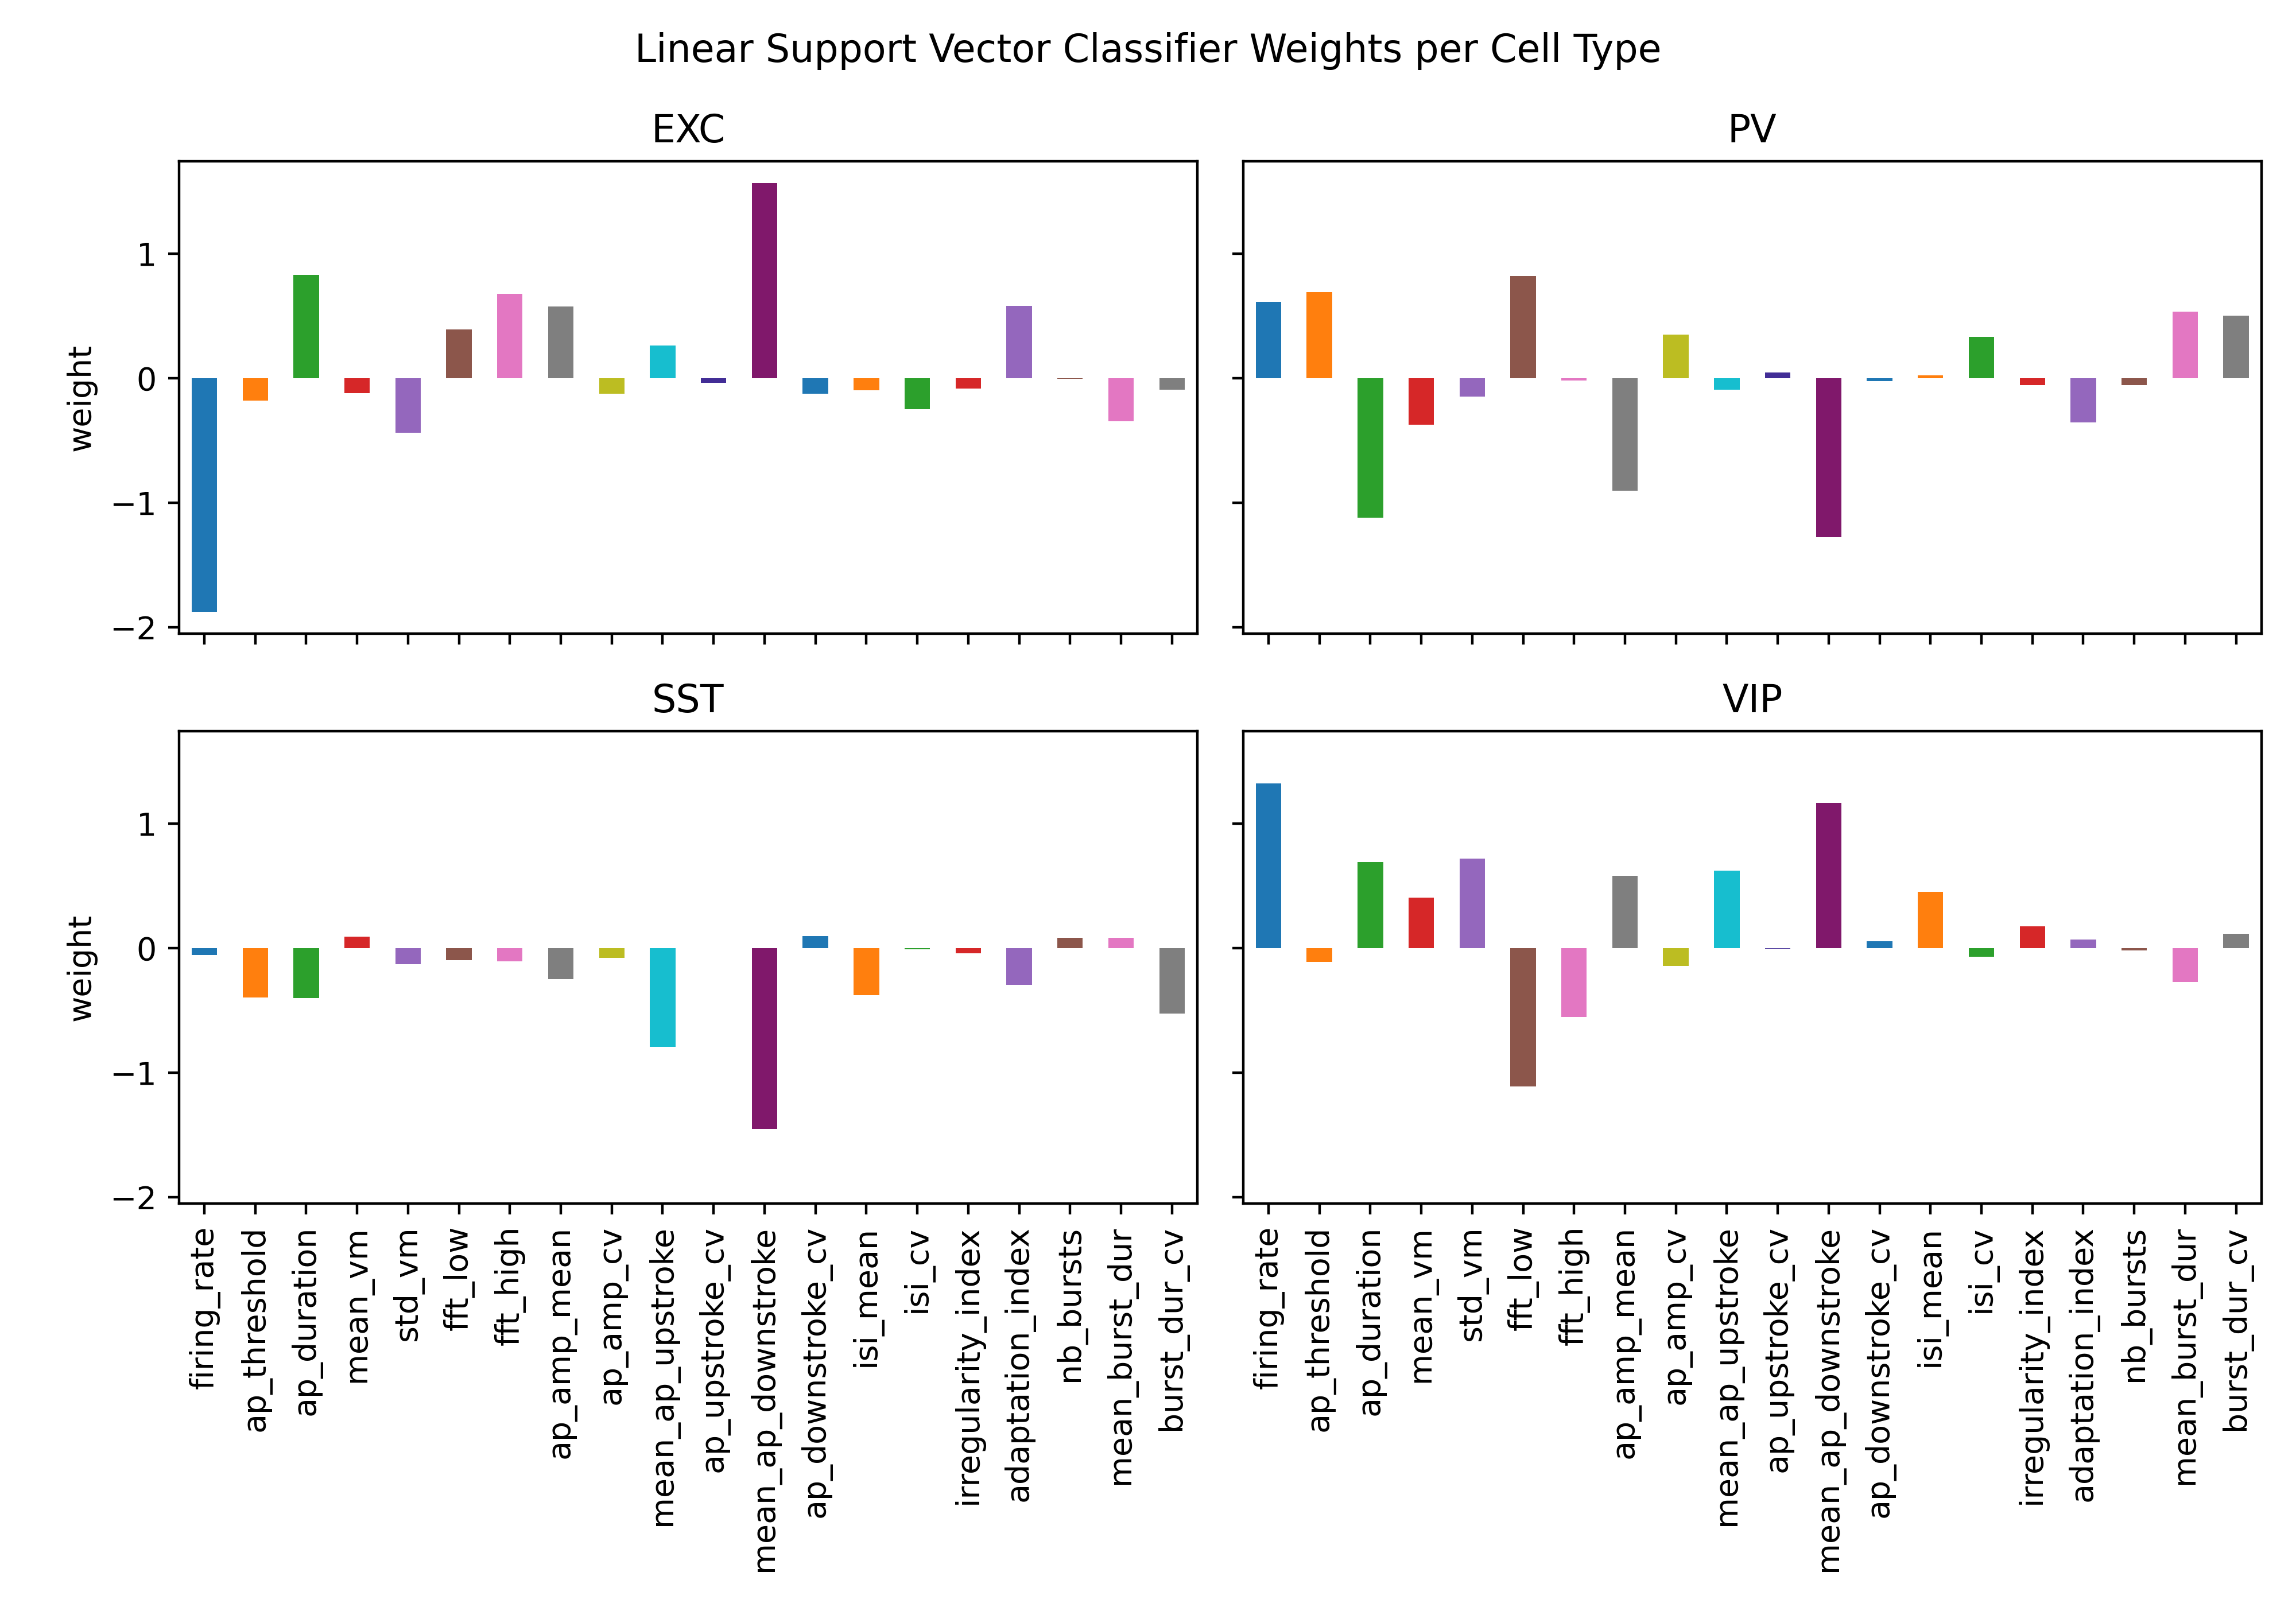
\includegraphics[width=0.9\columnwidth]{figures/weights_linearsvc.png}
  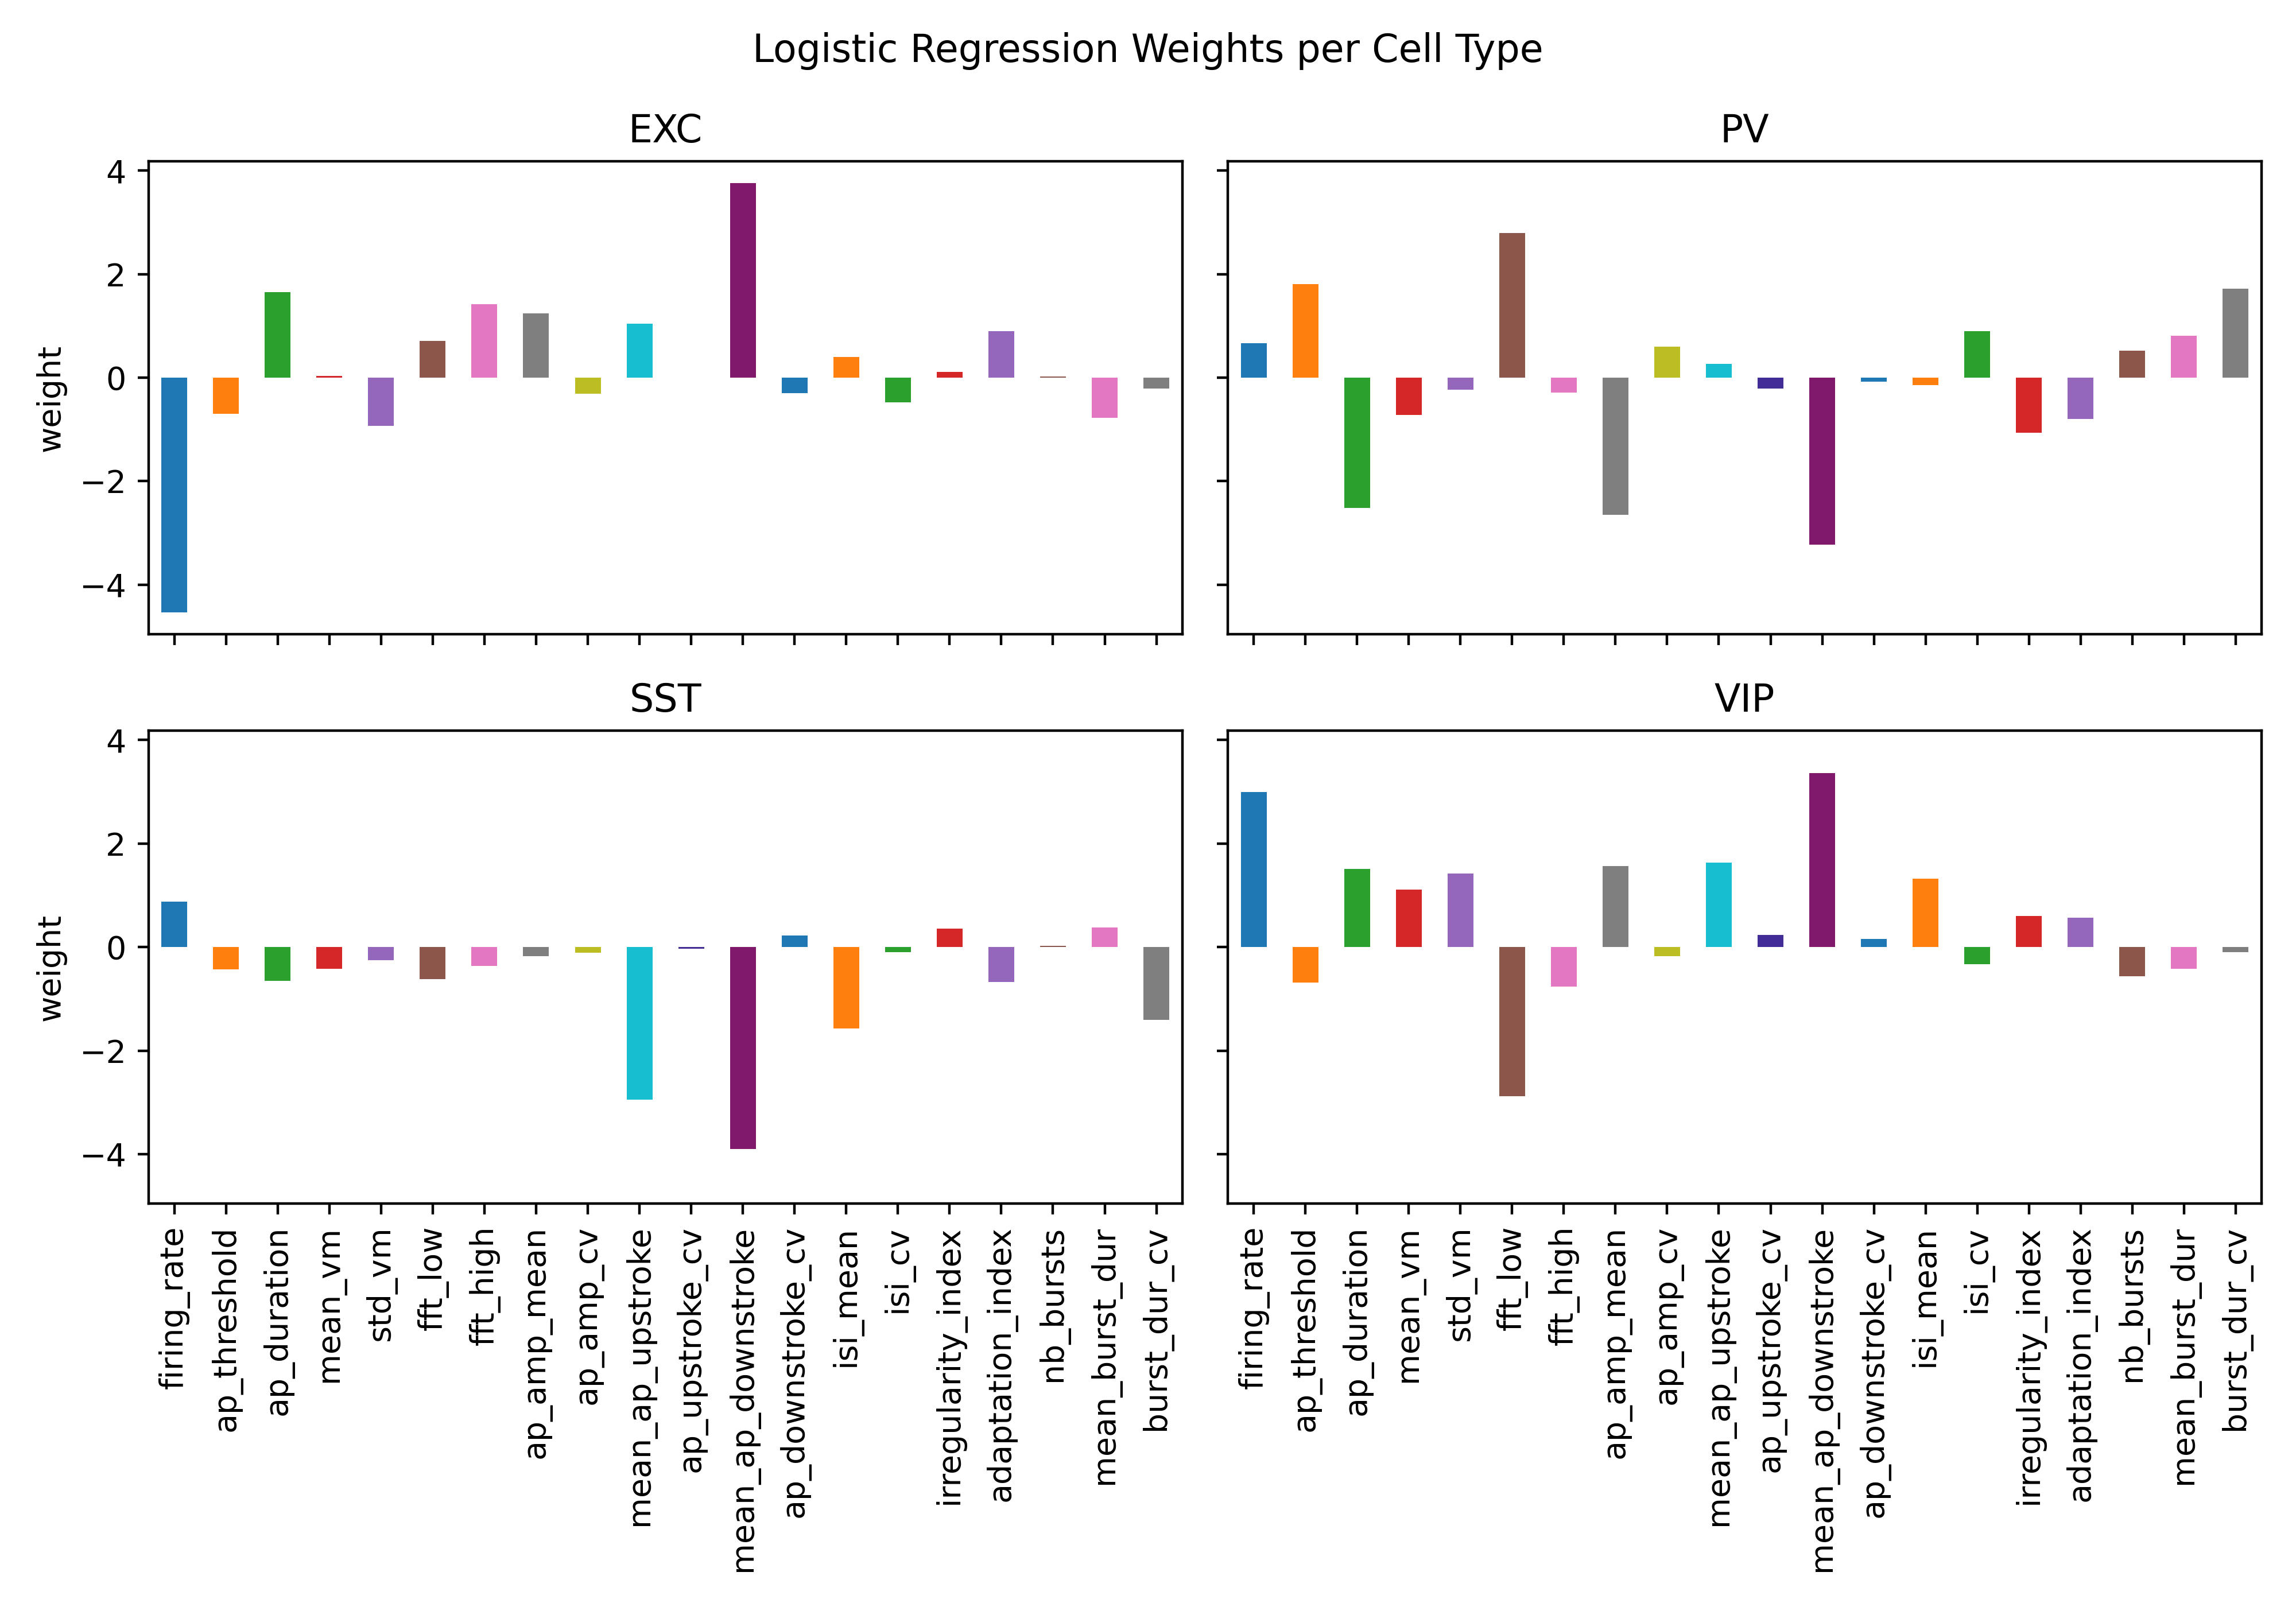
\includegraphics[width=0.9\columnwidth]{figures/weights_logistic_regression.png}
  \caption{Linear model weights across cell classes. Top four plots, are the weights of the Linear SVC (2nd best) and bottom four plots are the weights of the Logistic Regression (4th best).}%
  \label{fig:weights}
\end{figure*}

\subsubsection{Dimensionality Reduction}
Dimensionality reduction techniques were employed in order to visualize the data in lower dimensional sub-spaces (2D and 3D). Hence, we would be able to visualize whether there is a spatial arrangement between each cell class. The three employed techniques were Principal Component Analysis (PCA), t-distributed Stochastic Neighbor Embedding (t-SNE), and Uniform Manifold Approximation and Projection (UMAP).

\subsubsection{K-Means Clustering}
K-Means clustering algorithm was used in the lower dimensional subspace projections of our data. We fixed K to be equal to the number of cell classes present ($K=4$), in order to determine whether each cluster could represent a specific cell class.

%-----------------------------------------------------


\section{Results}

\subsection{Best Models}

\begin{figure}[h!]
  \centering
  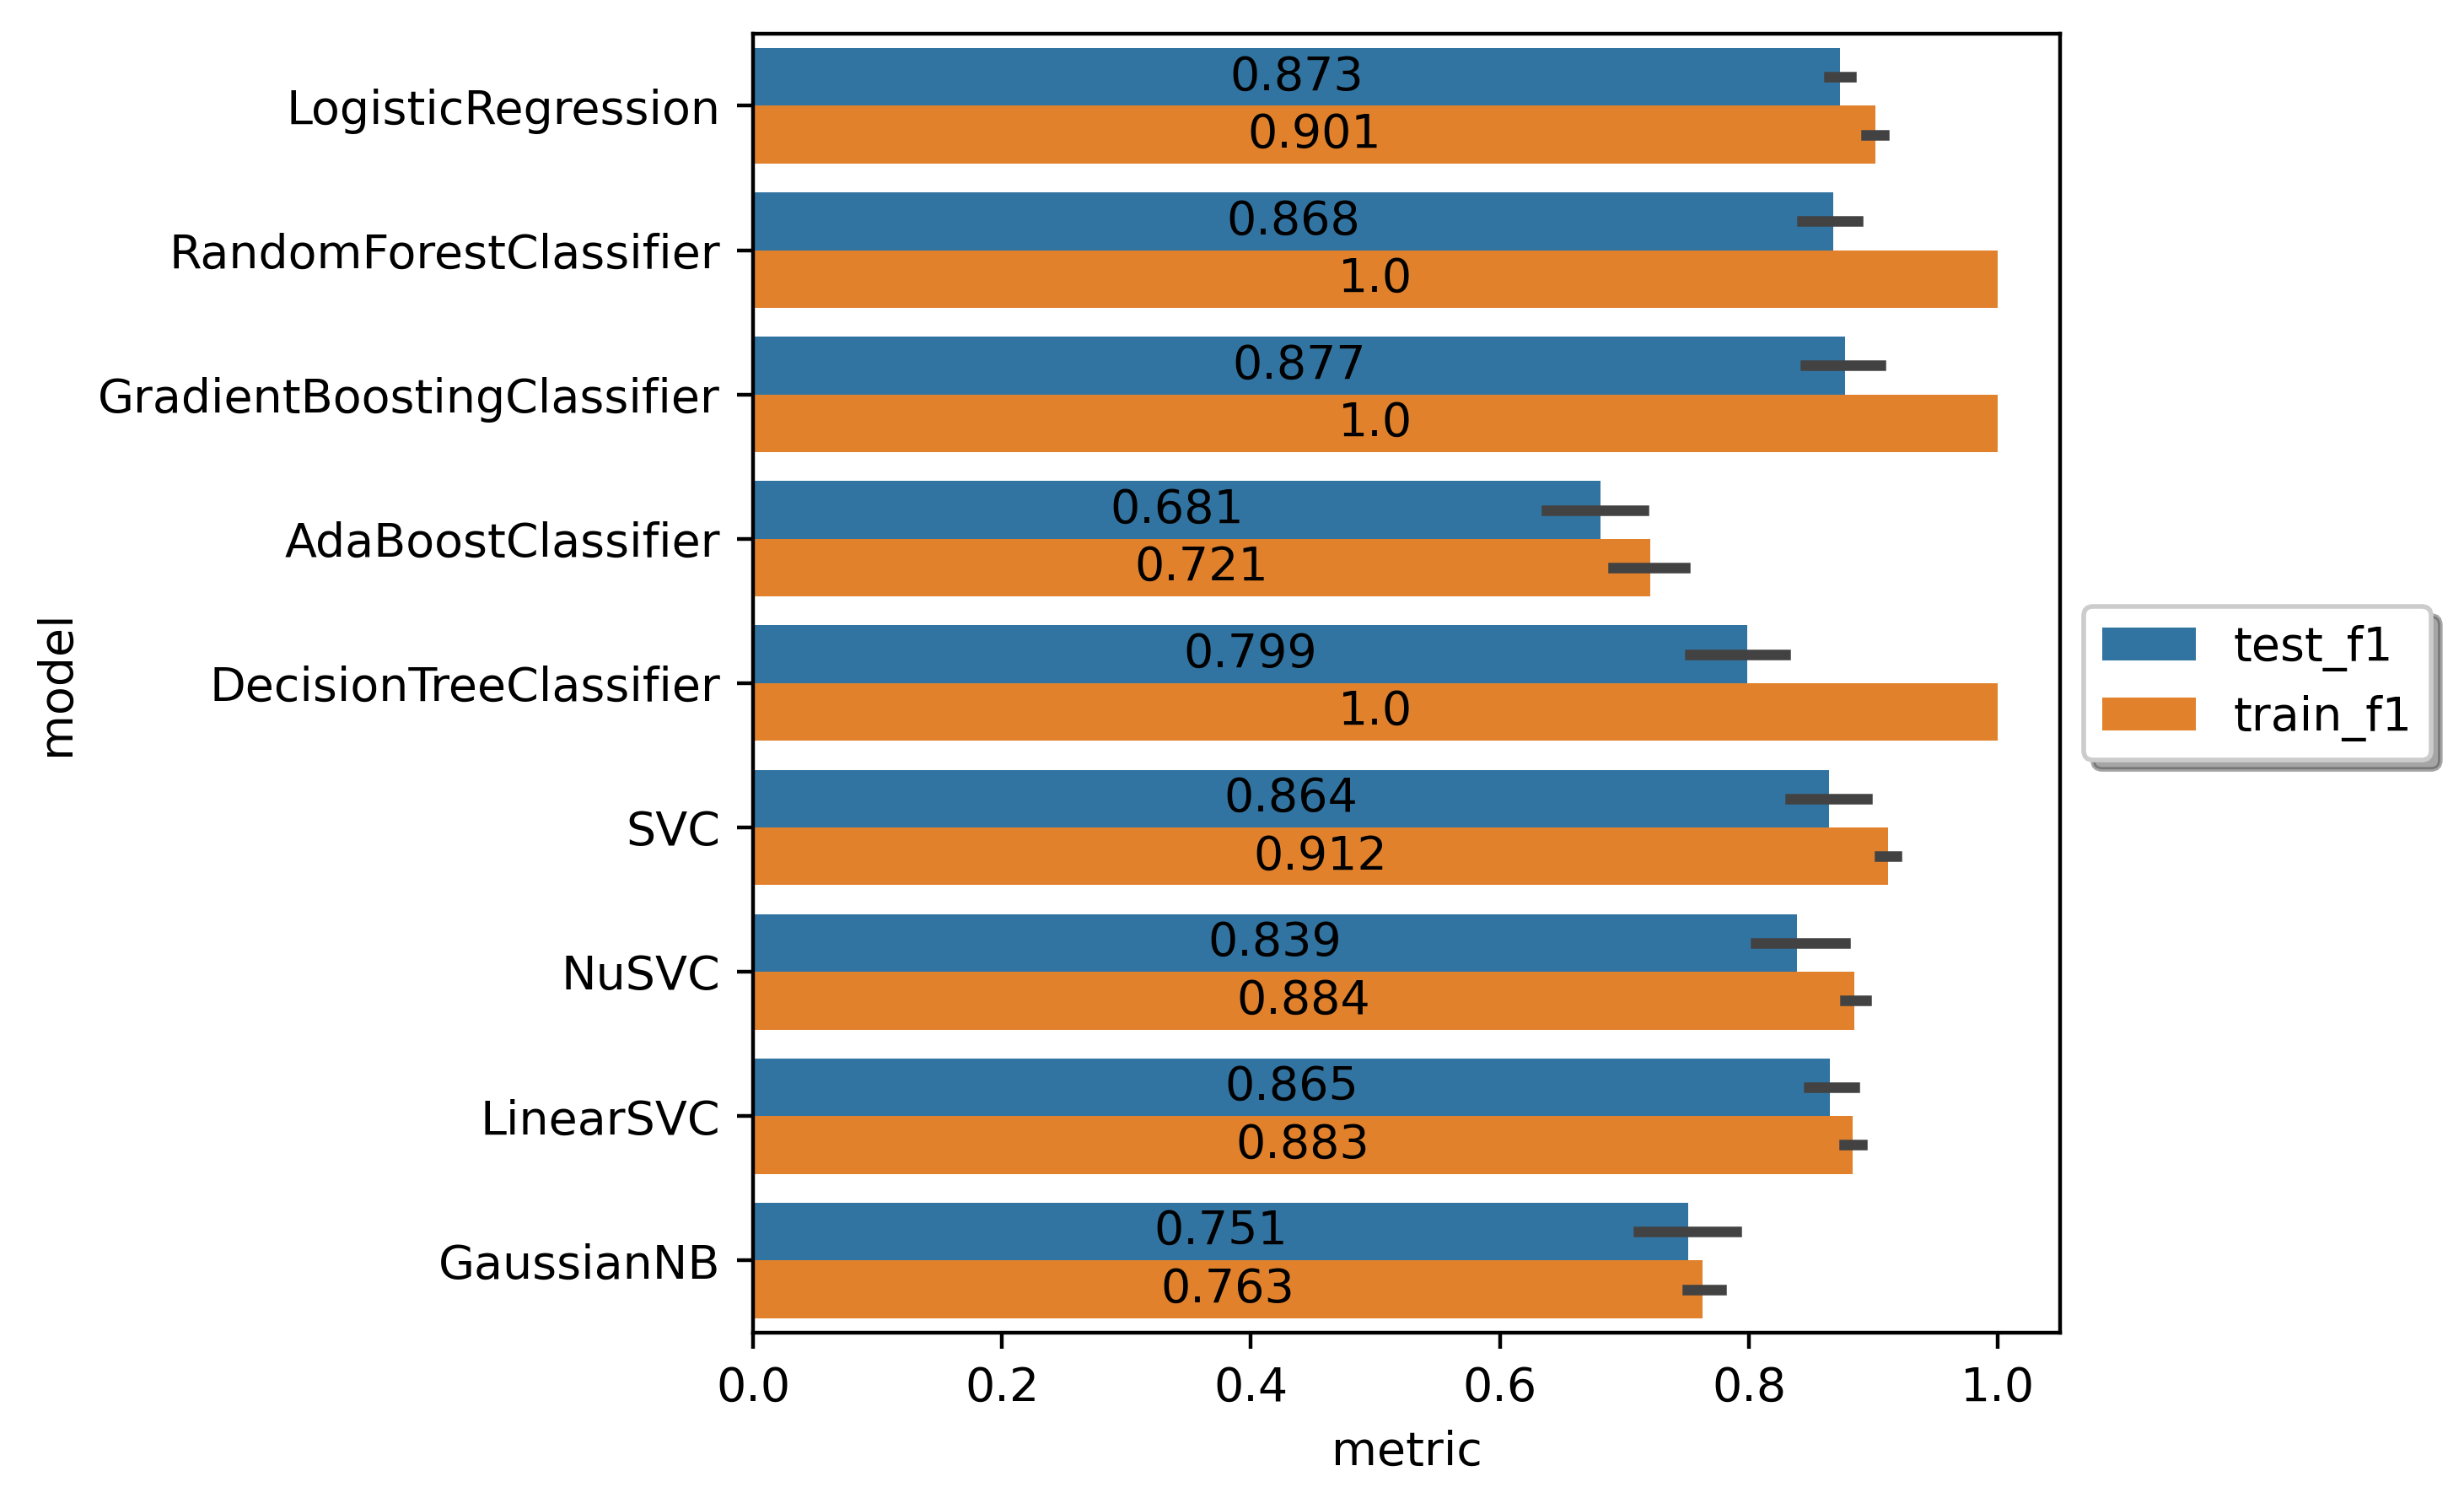
\includegraphics[width=\columnwidth]{figures/models_unturned_f1.png}
  \caption{F1 score performances, on a stratified 5-Fold CV, for a range of models tested.}
  \label{fig:models_untuned}
\end{figure}

\begin{table}[h!]
  \centering
  \begin{tabular}{|l|l|l|l|}
  \hline
  \textbf{Model} & \textbf{Inference} & \textbf{Mean} & \textbf{Std} \\
  \hline
  Gradient Boosting & Test & 0.8888 & 0.0366 \\
   & Train & 1.0 & 0.0 \\
  \hline
  Linear Support Vector Machine & Test & 0.8832 & 0.0090 \\
   & Train & 0.9094 & 0.0125 \\
  \hline
  Random Forest & Test & 0.8789 & 0.0334 \\
   & Train & 1.0 & 0.0 \\
  \hline
  Logistic Regression & Test & 0.8756 & 0.0188 \\
   & Train & 0.9166 & 0.0136 \\
  \hline
  Ensemble & Test & 0.9065 & 0.0206 \\
   & Train & 0.9631 & 0.0072 \\
  \hline
  \end{tabular}
  \caption{Stratified 5-fold CV F1 score performance of top 4 best (HPO) models, plus the ensemble combination of them.}
  \label{tab:best_model_scores}
\end{table}

From Fig. \ref{fig:models_untuned} we can see that the four best unoptimized models, based on test performance, are: 1st GradientBoosting with a score of $0.877$, 2nd Logistic Regression, 3rd Random Forest and 4th Linear SVC. After having done HPO (Table-\ref{tab:best_model_scores}), these models improve by about 1 to 2 \%, every model is now above $0.8756$, and Linear SVC and Logistic Regression swap places. Furthermore, by ensembling these four best models, it is possible to increase test performance by an additional  1.77 \% (from $0.8888 \pm 0.0366$ to $0.9065 \pm 0.0206$).
It is interesting to notice that tree-based methods (Gradient Boosting and Random Forest) overfit to a greater extent, and have a higher standard deviation than linear models.

\begin{figure}[h!]
  \centering
  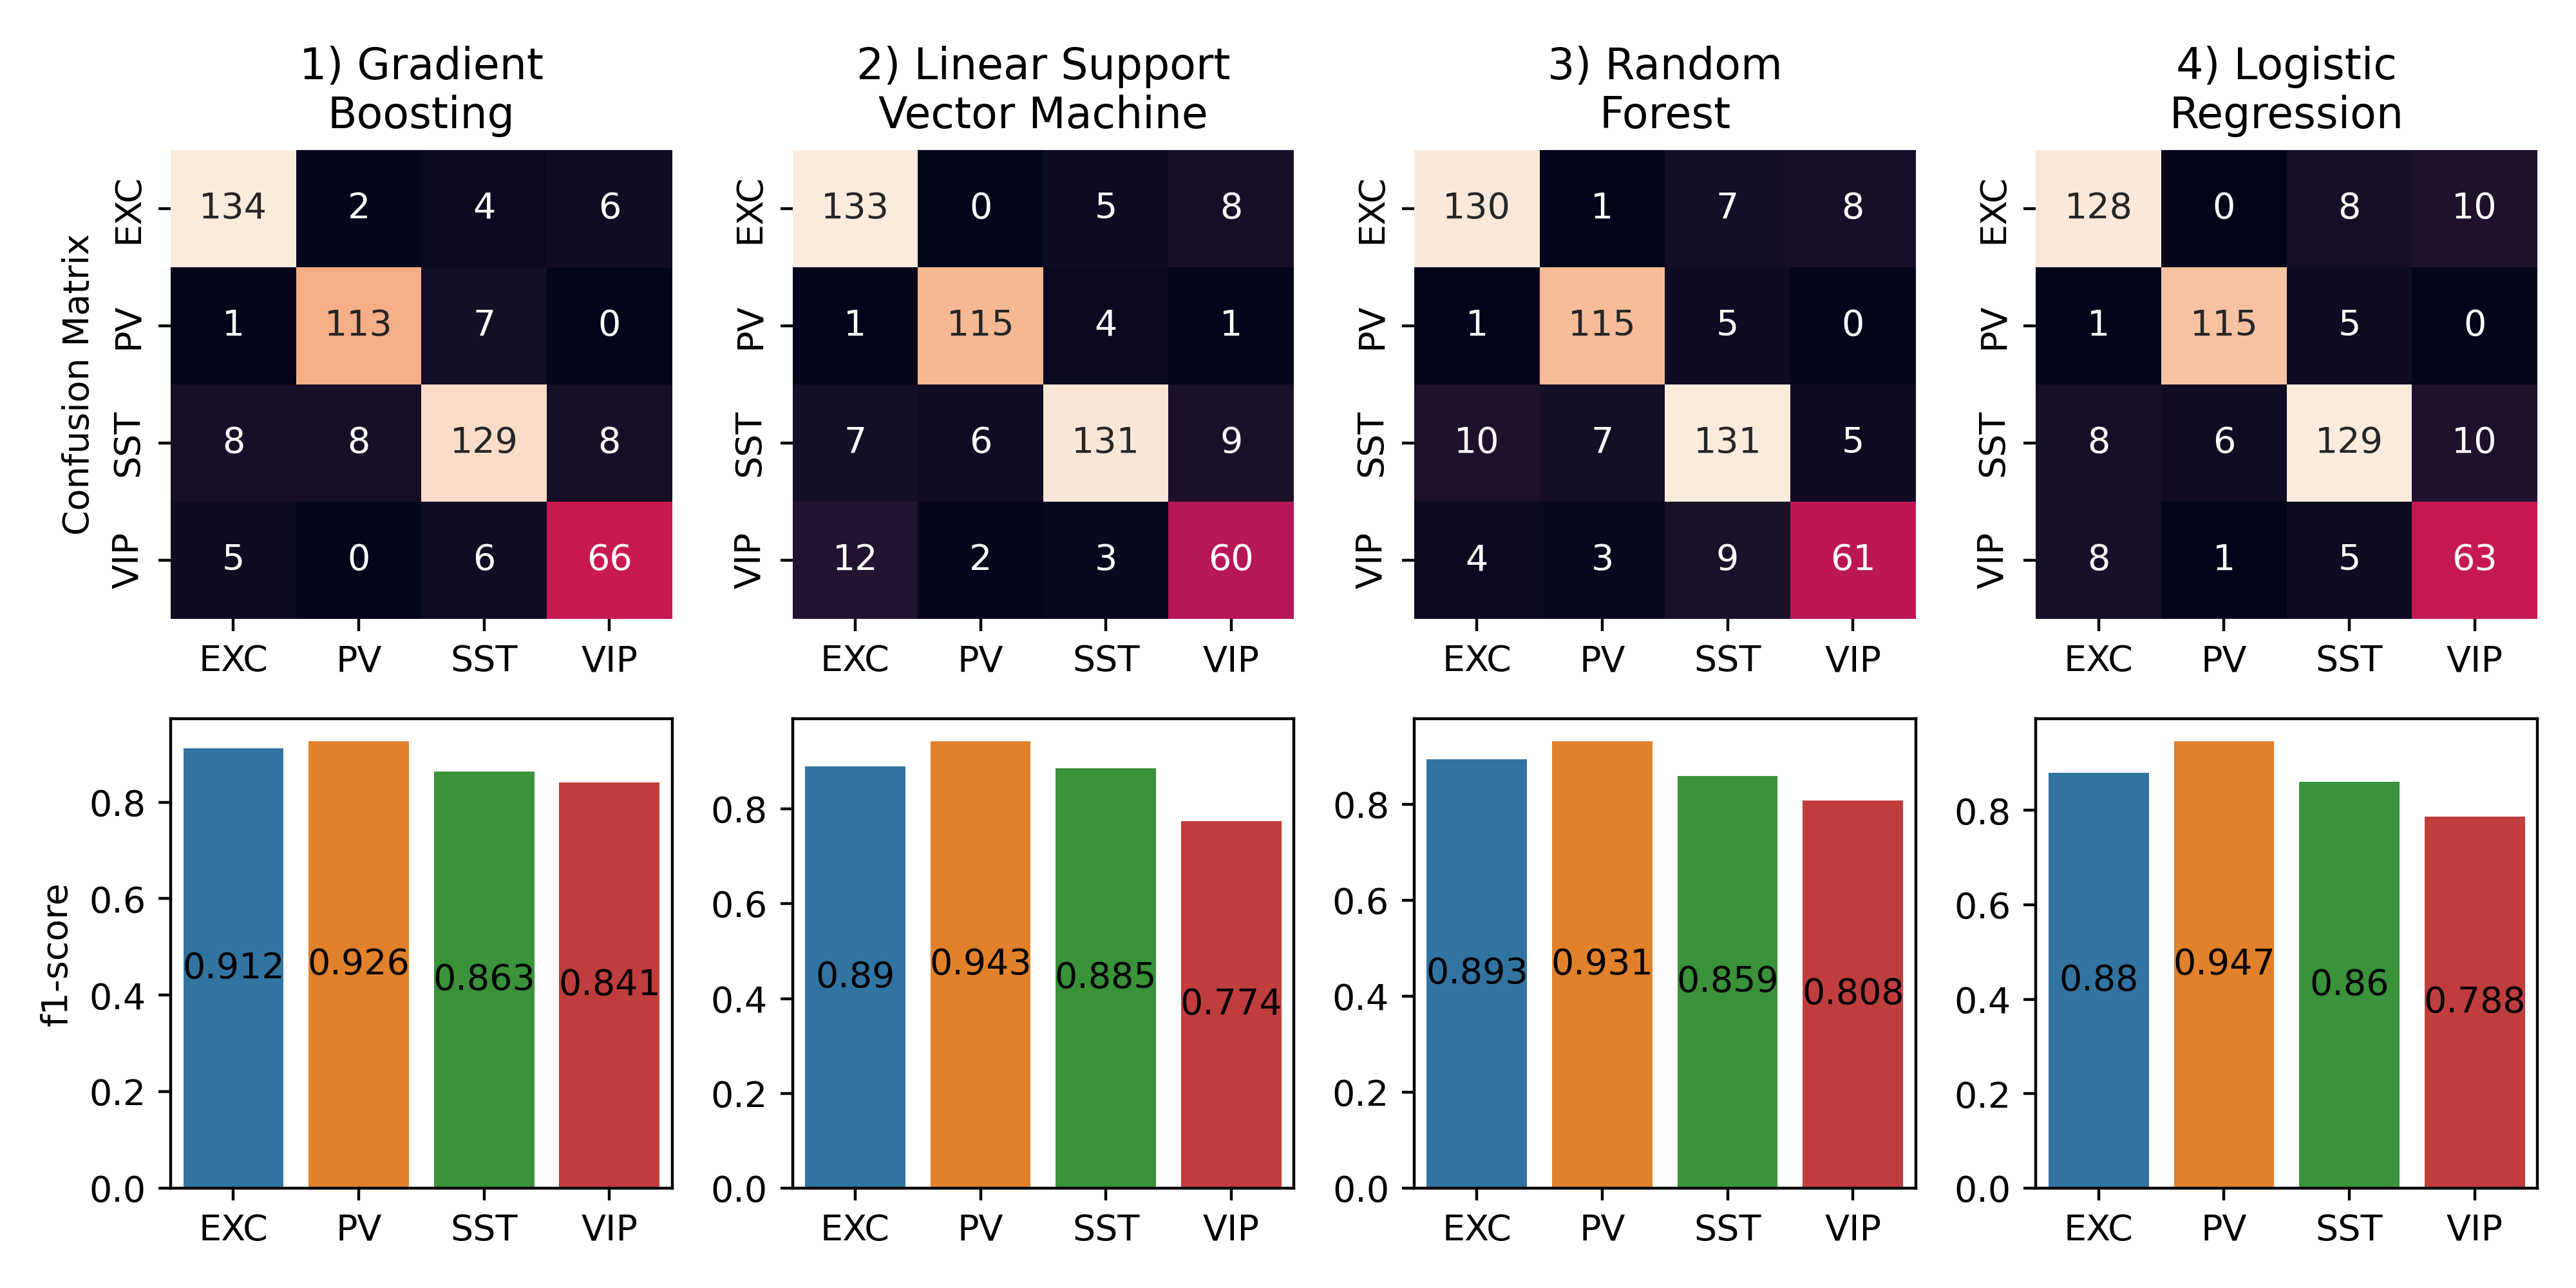
\includegraphics[width=\columnwidth]{figures/confusion_matrices_of_classifiers.png}
  \caption{Top 4 best model performances. Each column correspond to a model. Top row are confusion matrices based on a 5-Fold Stratified CV prediction. For each one of them the x-axis corresponds to predictions and the y-axis to the ground truth. Bottom row are the F1 scores for each cell type, calculated with the same prediction.}
  \label{fig:supervised_confusion_matrices}
\end{figure}

In Fig. \ref{fig:supervised_confusion_matrices} we can see that VIP cells cannot be classified as well as the others. This is consistent throughout each model, with the VIP $F1$ score being $0.841$, $0.774$, $0.808$ and $0.788$, respectively from best to worst ranked classifier. 
On the other hand PV cells are by far the best classified cell class, followed by EXC and then by SST cells. When we look at the miss-classified VIP cells 3 out of 4 times, none are classified as PV. Only one EXC cell is miss-classified as a PV cell.



\subsection{Feature Importance}

\subsubsection{Gradient Boosting}
For the Gradient Boosting Classifier the 5 most significant features are: the number of bursts, the AP duration, the highest amplitude of the Fourier transform, the firing rate and the mean of the membrane potential (Fig. \ref{fig:feature_importances}).

\subsubsection{Linear SVC}
For the Linear SVC model, the 5 most significant features are: the mean AP downstroke, the firing rate, AP duration, the lowest amplitude of the Fourier transform, and the AP amplitude mean (Fig. \ref{fig:feature_importances}).
More specifically if we look at the weight of each feature to determine the cell type (Fig. \ref{fig:weights}), there is a positive correlation with AP downstroke for EXC and VIP cells, versus negative for PV and SST cells. The firing rate is highly negatively correlated with EXC, positively for PV and VIP, and close to no correlation for SST cells. AP duration is positively correlated with EXC and VIP whereas negative for PV and SST.

\subsubsection{Random Forest}
For the Random Forest Classifier the 5 most significant features are: the AP duration, the number of bursts, the firing rate, the mean inter-spike intervals and the highest amplitude of the Fourier transform, (Fig. \ref{fig:feature_importances}).

\subsubsection{Logistic Regression}
For the Linear SVC model, the 5 most significant features are the mean AP downstroke, the firing rate, the lowest amplitude of the Fourier transform, AP duration, and the mean AP upstroke.
(Fig. \ref{fig:feature_importances}).
More specifically if we look at the weight of each feature to determine the cell type (Fig. \ref{fig:weights}), the same observations as the linear SVC can be made.


\subsection{Dimensionality Reduction}

\begin{figure}[h!]
  \centering
  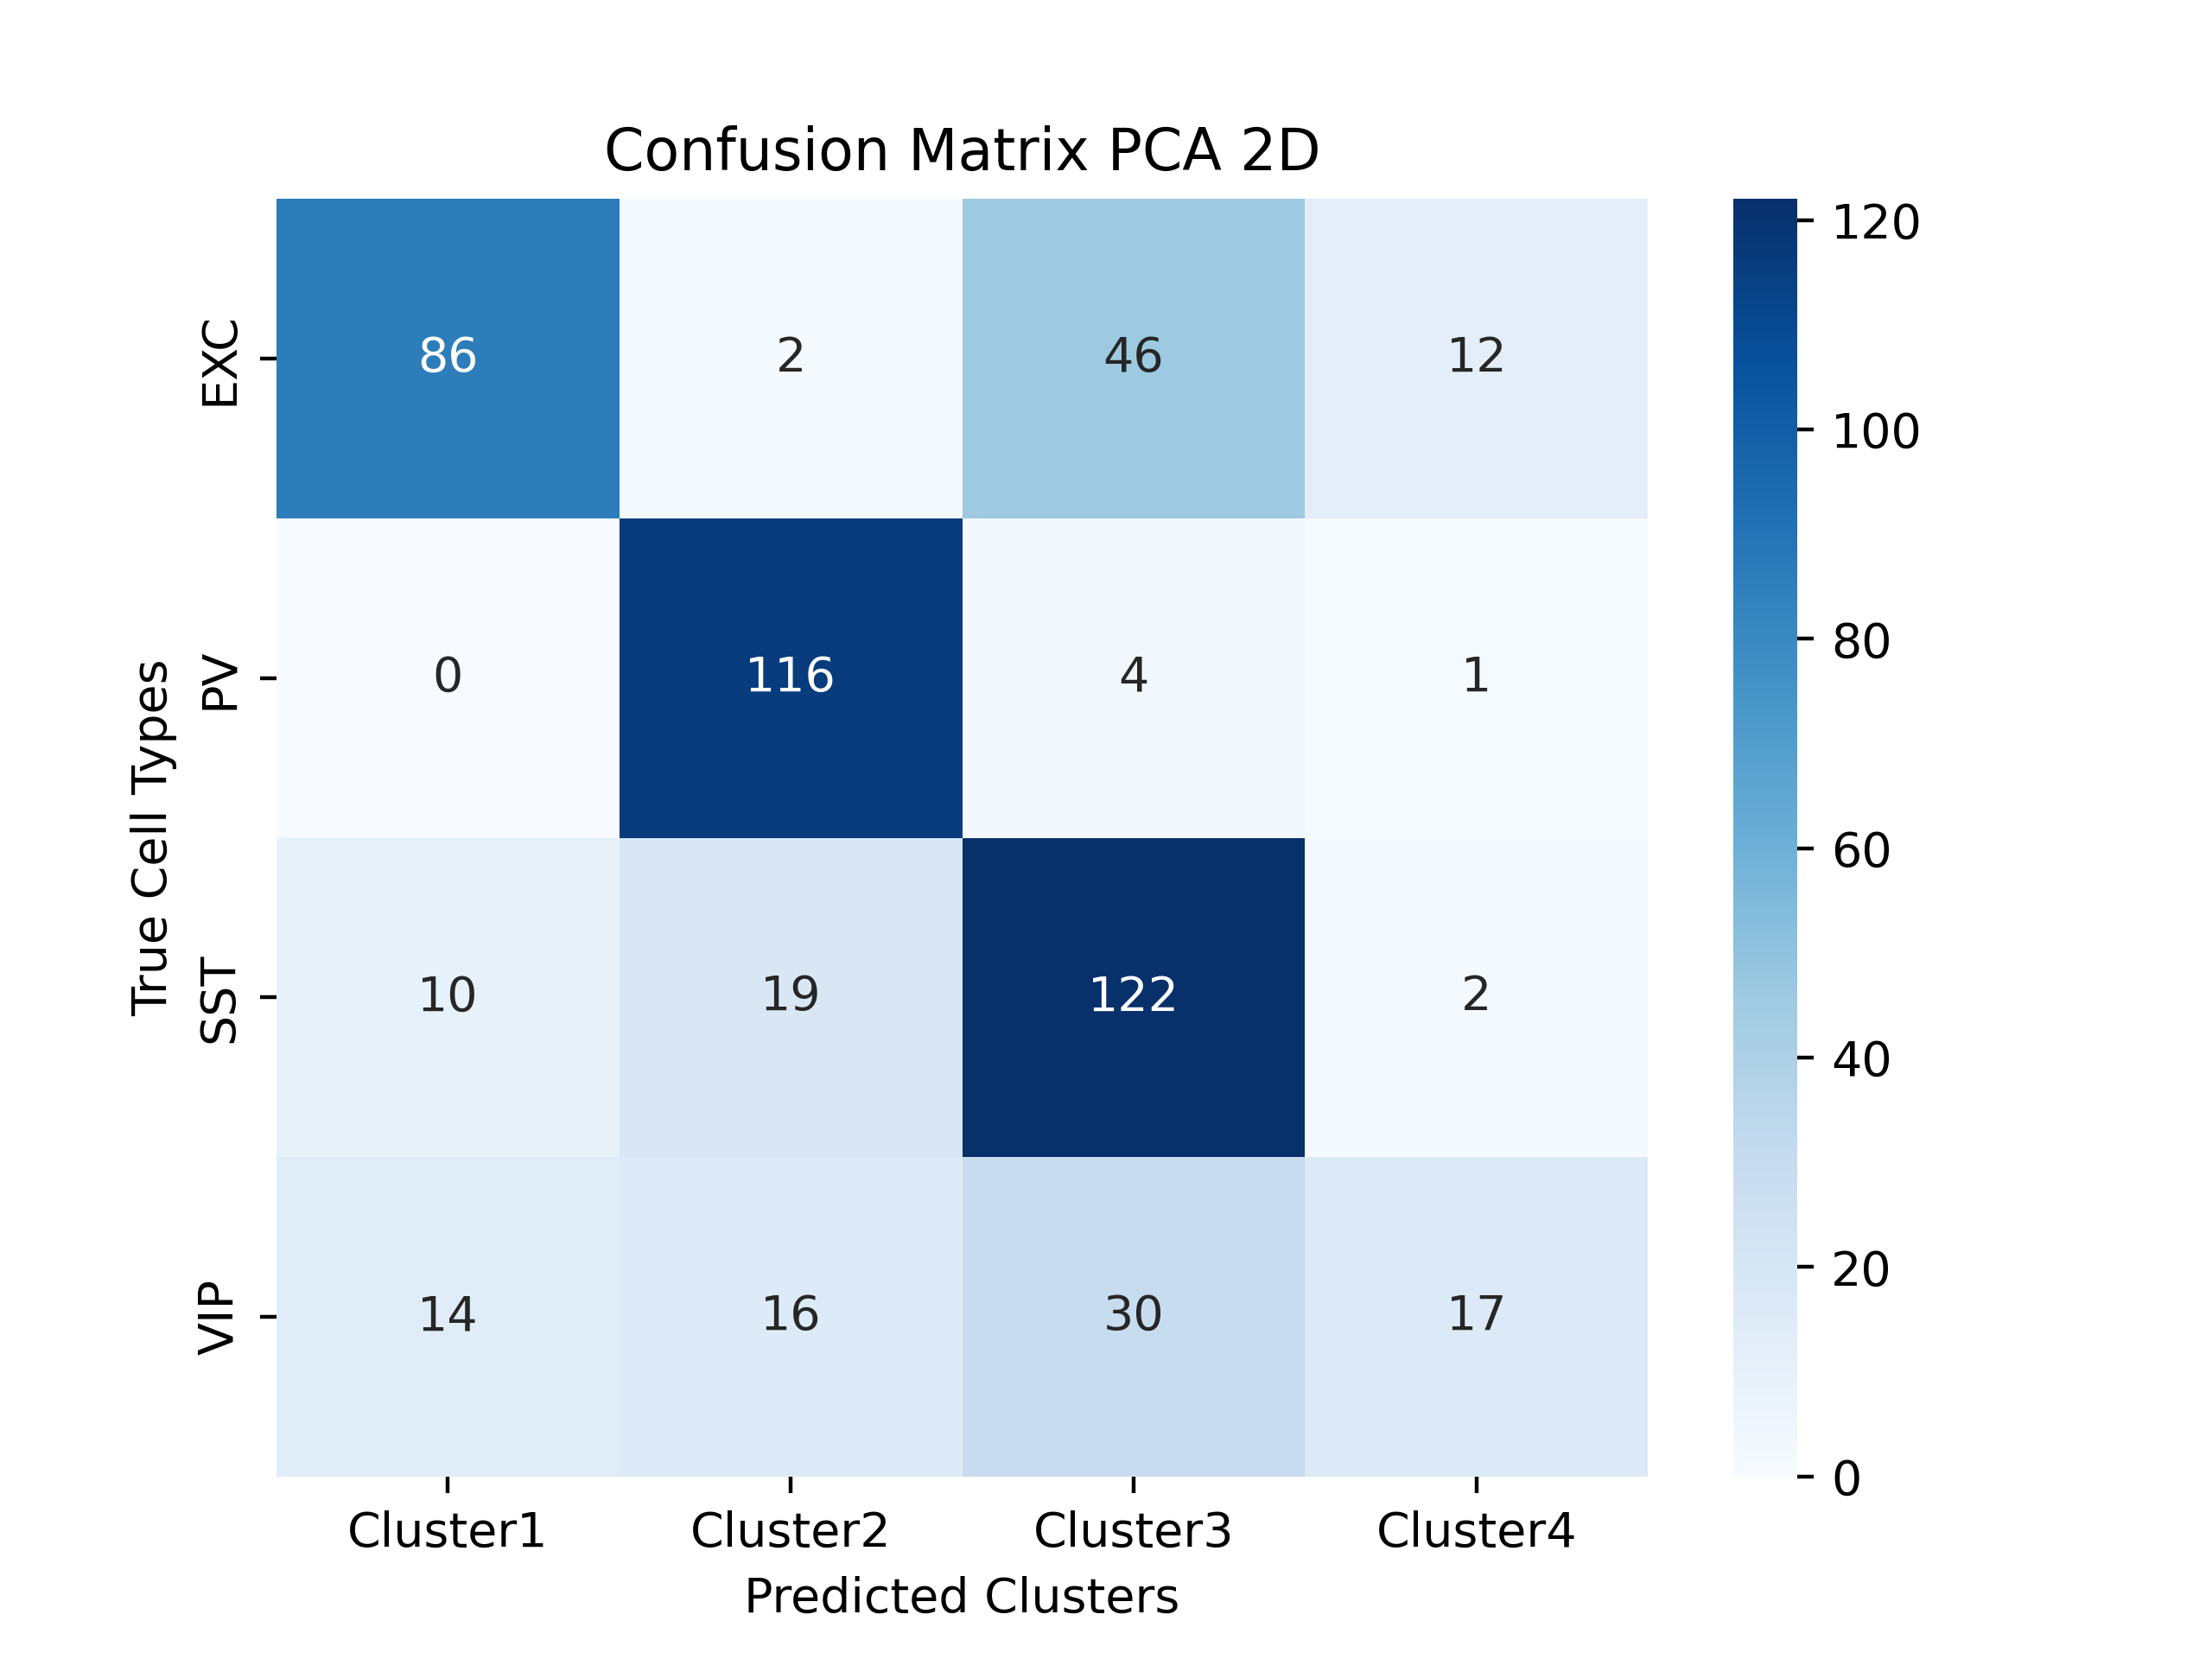
\includegraphics[width=0.45\columnwidth]{figures/Confusion Matrix PCA 2D.png}
  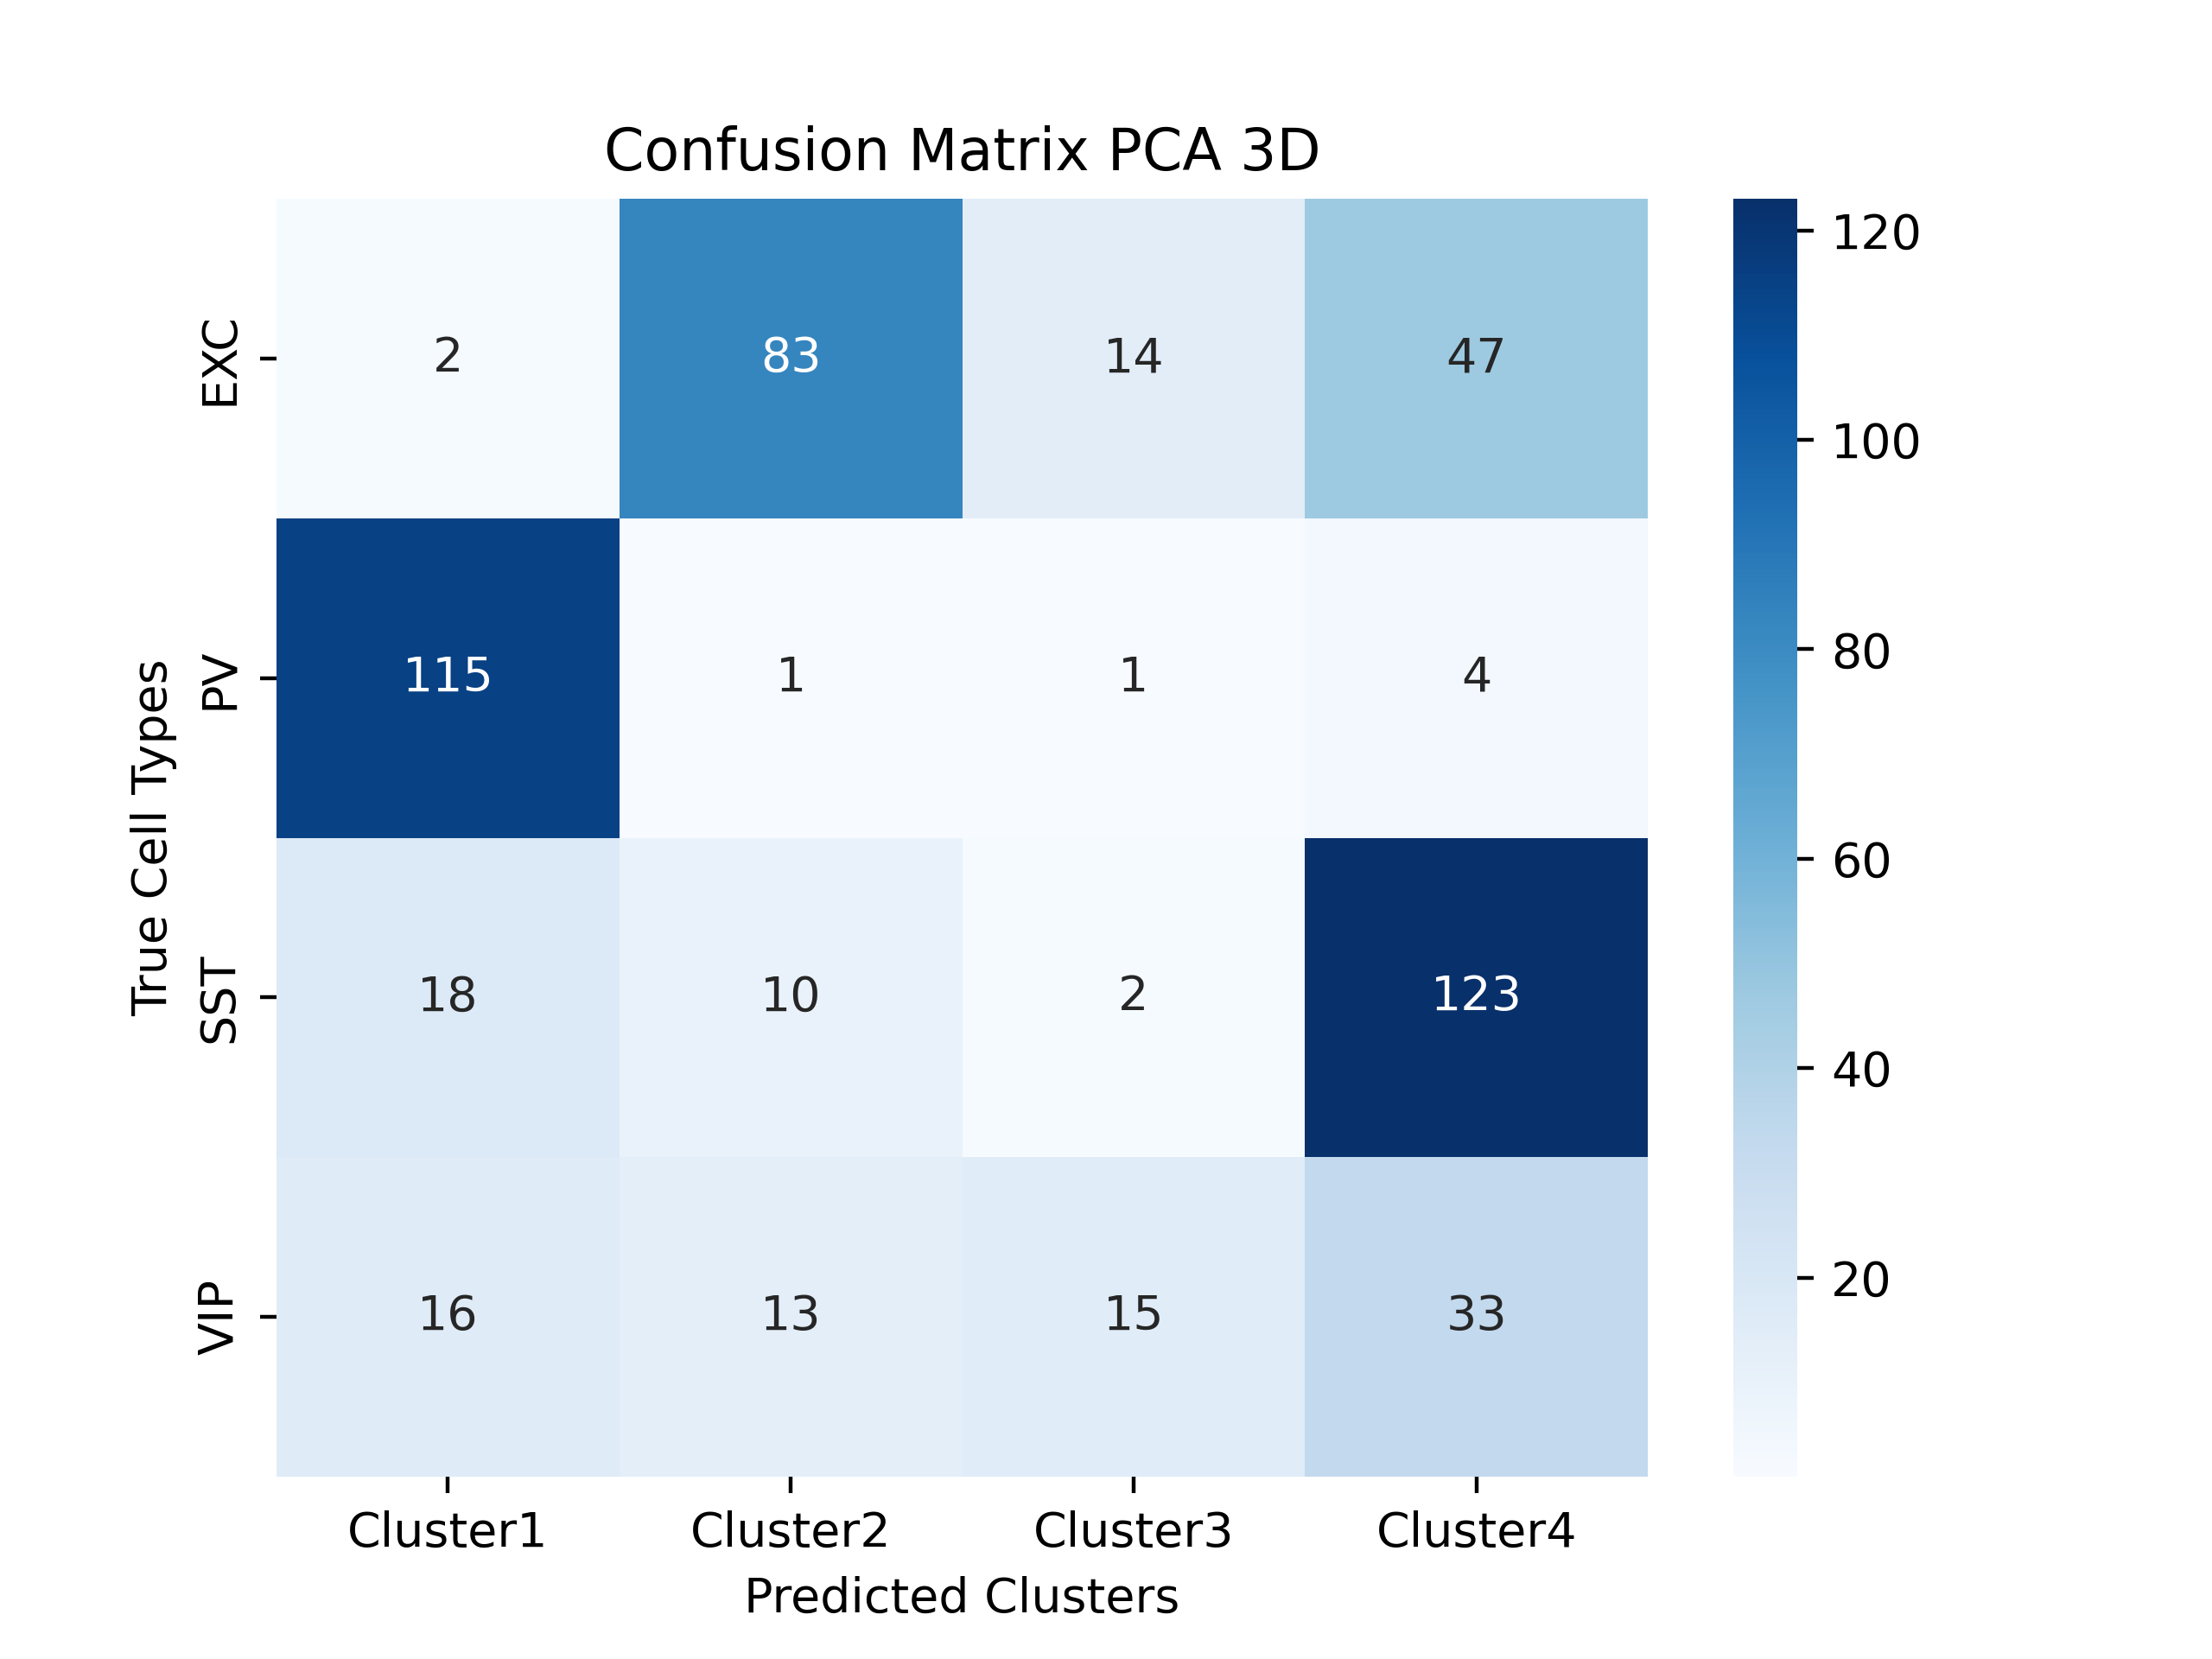
\includegraphics[width=0.45\columnwidth]{figures/Confusion Matrix PCA 3D.png}
  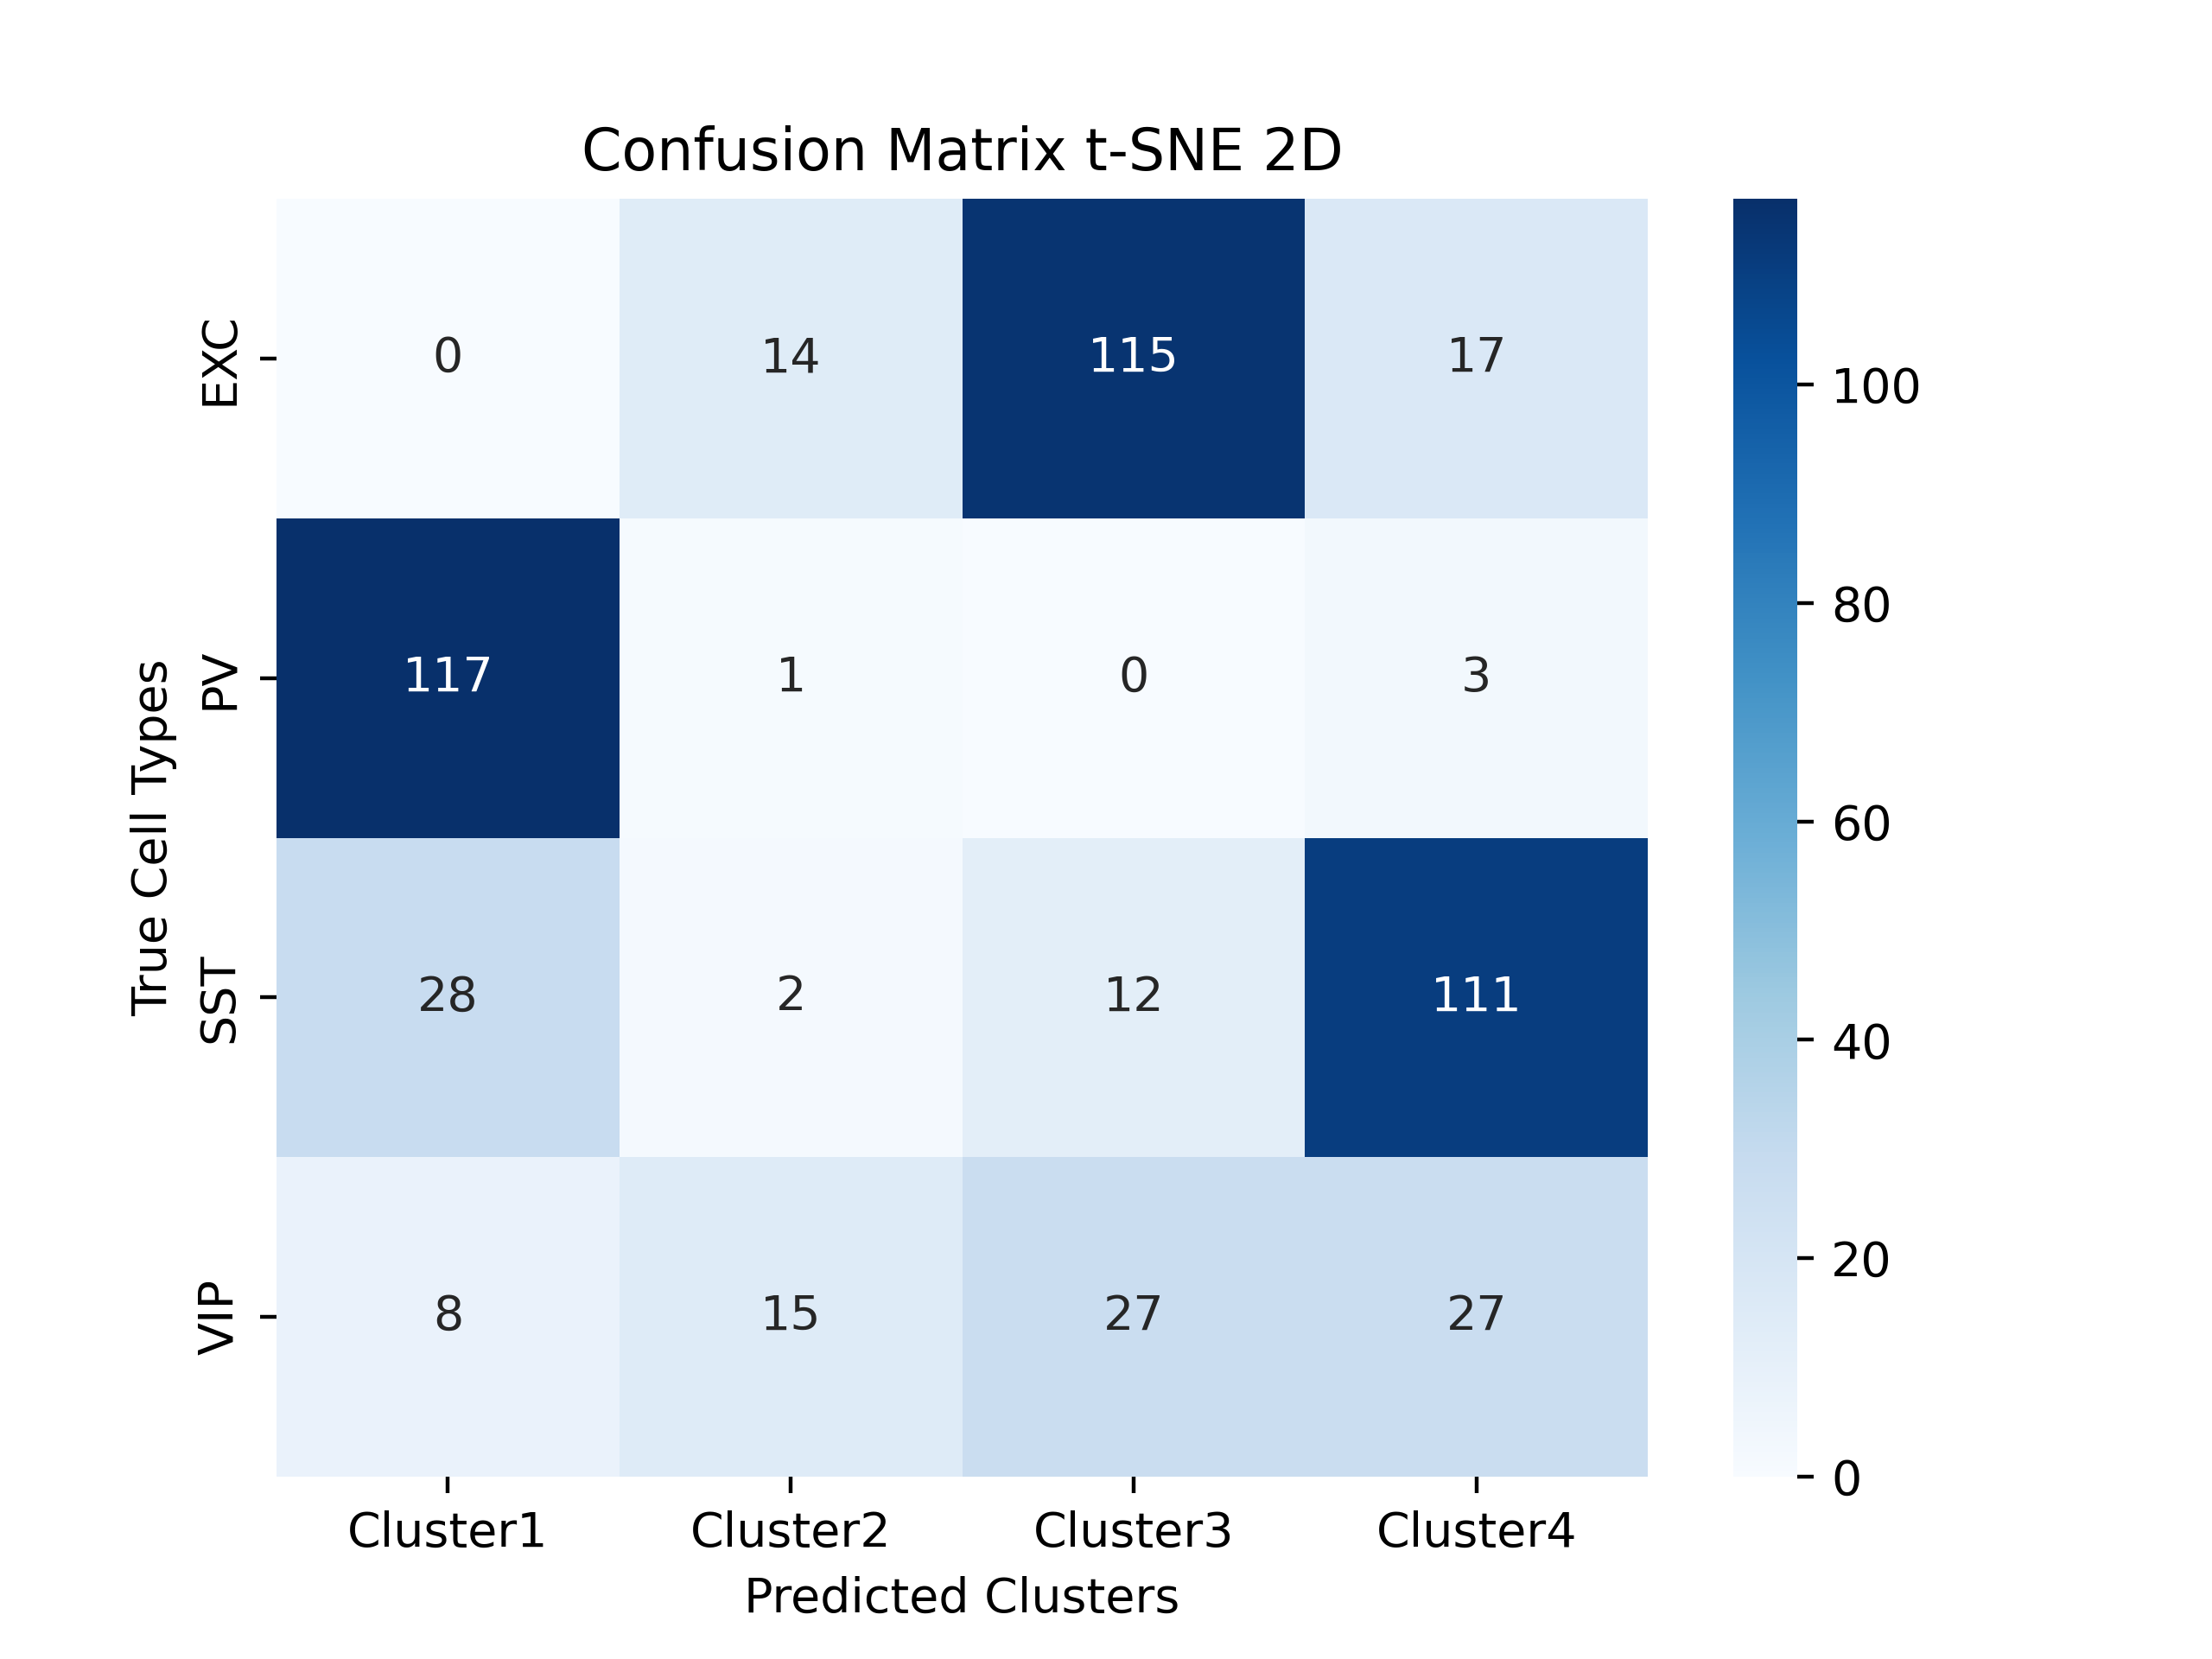
\includegraphics[width=0.45\columnwidth]{figures/Confusion Matrix t-SNE 2D.png}
  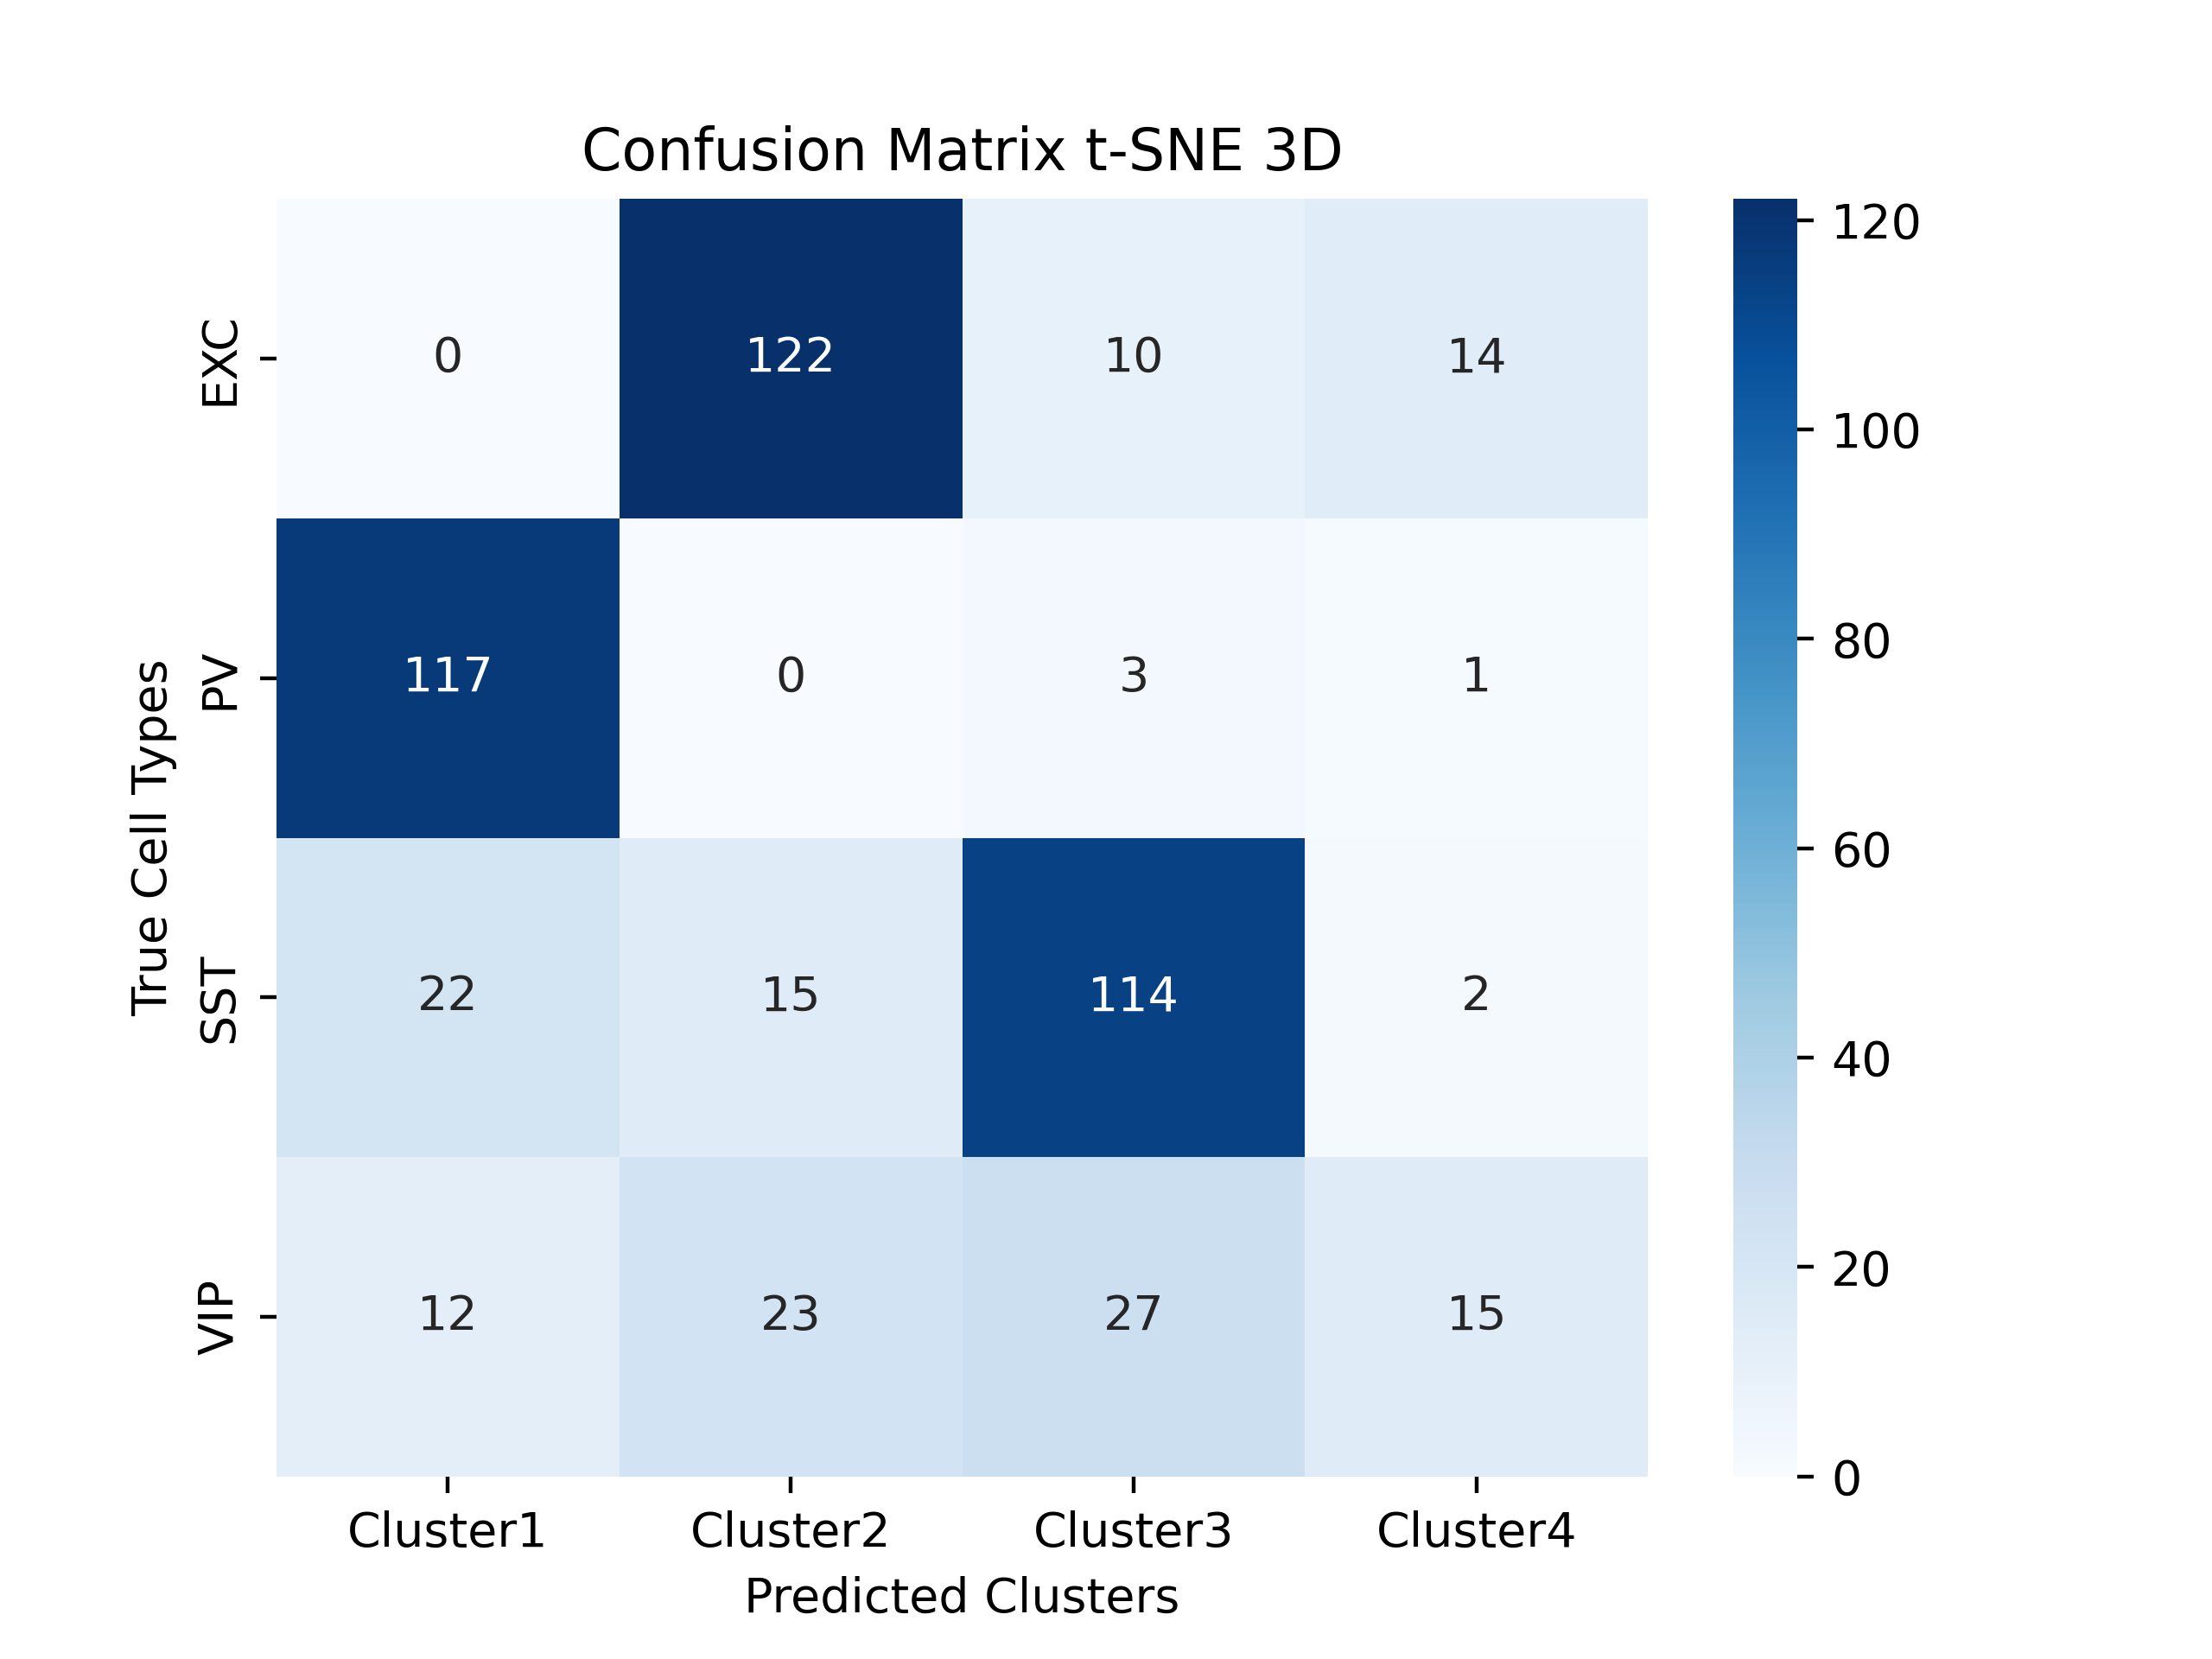
\includegraphics[width=0.45\columnwidth]{figures/Confusion Matrix t-SNE 3D.png}
  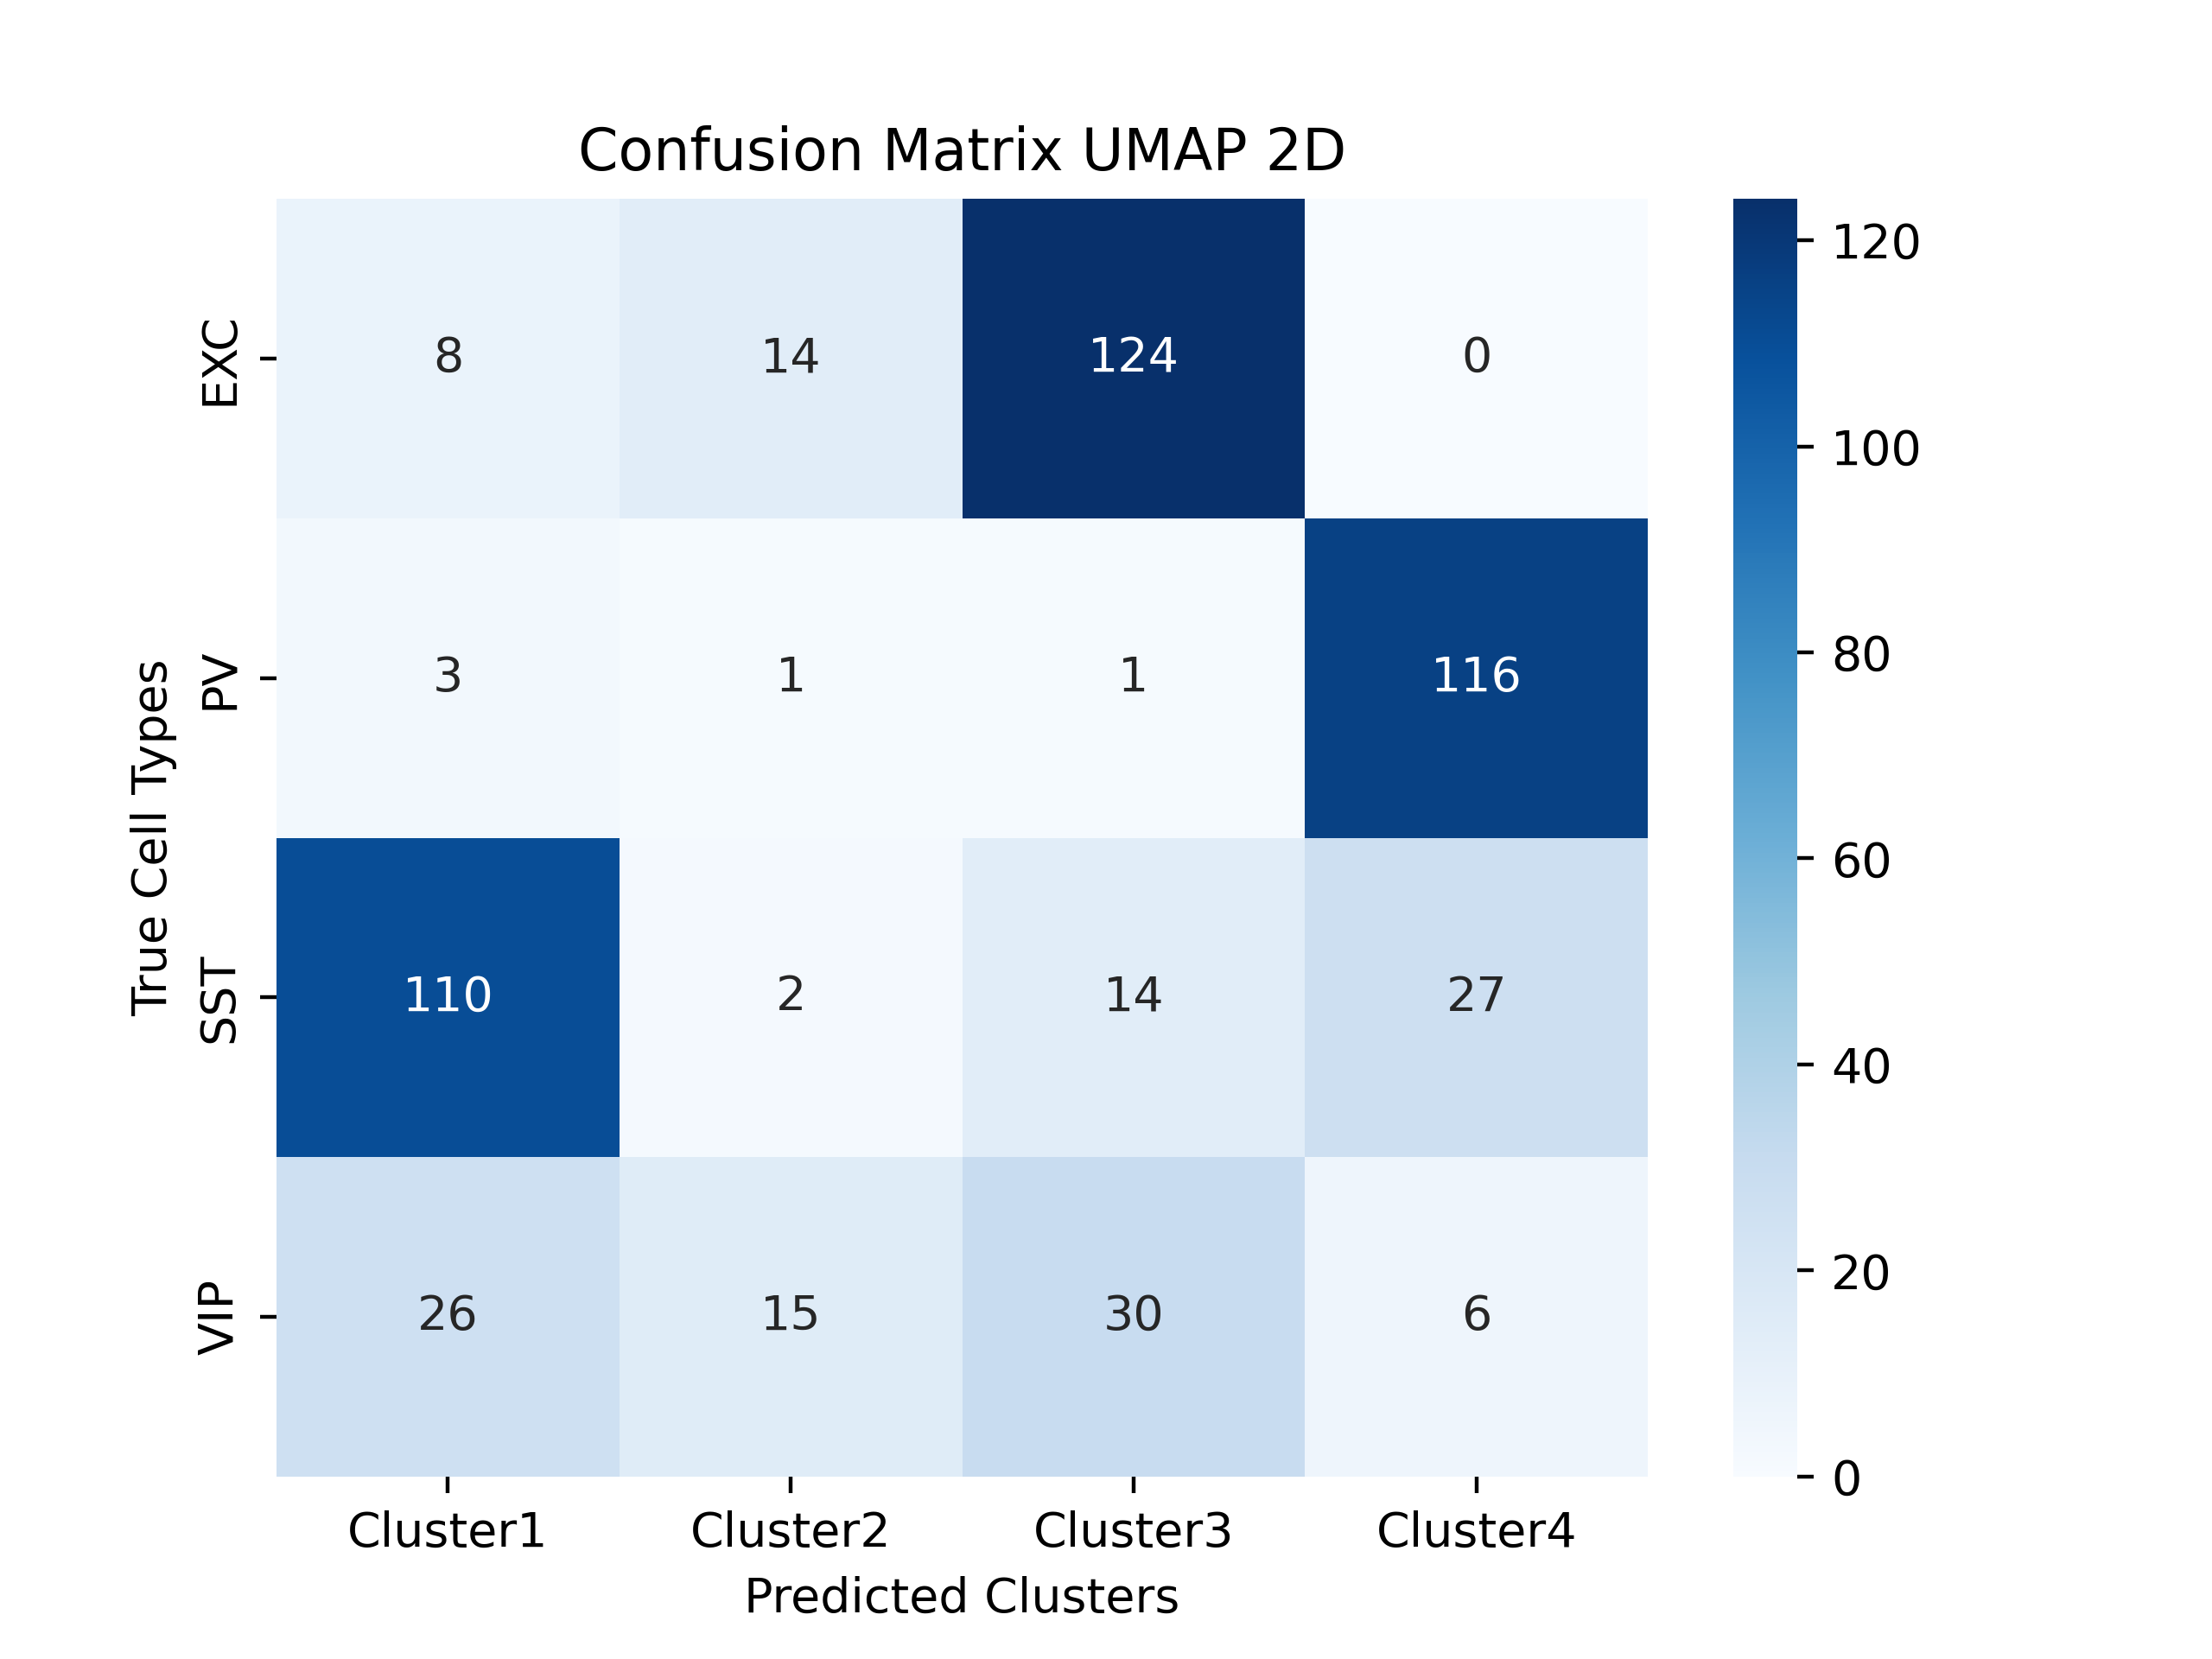
\includegraphics[width=0.45\columnwidth]{figures/Confusion Matrix UMAP 2D.png}
  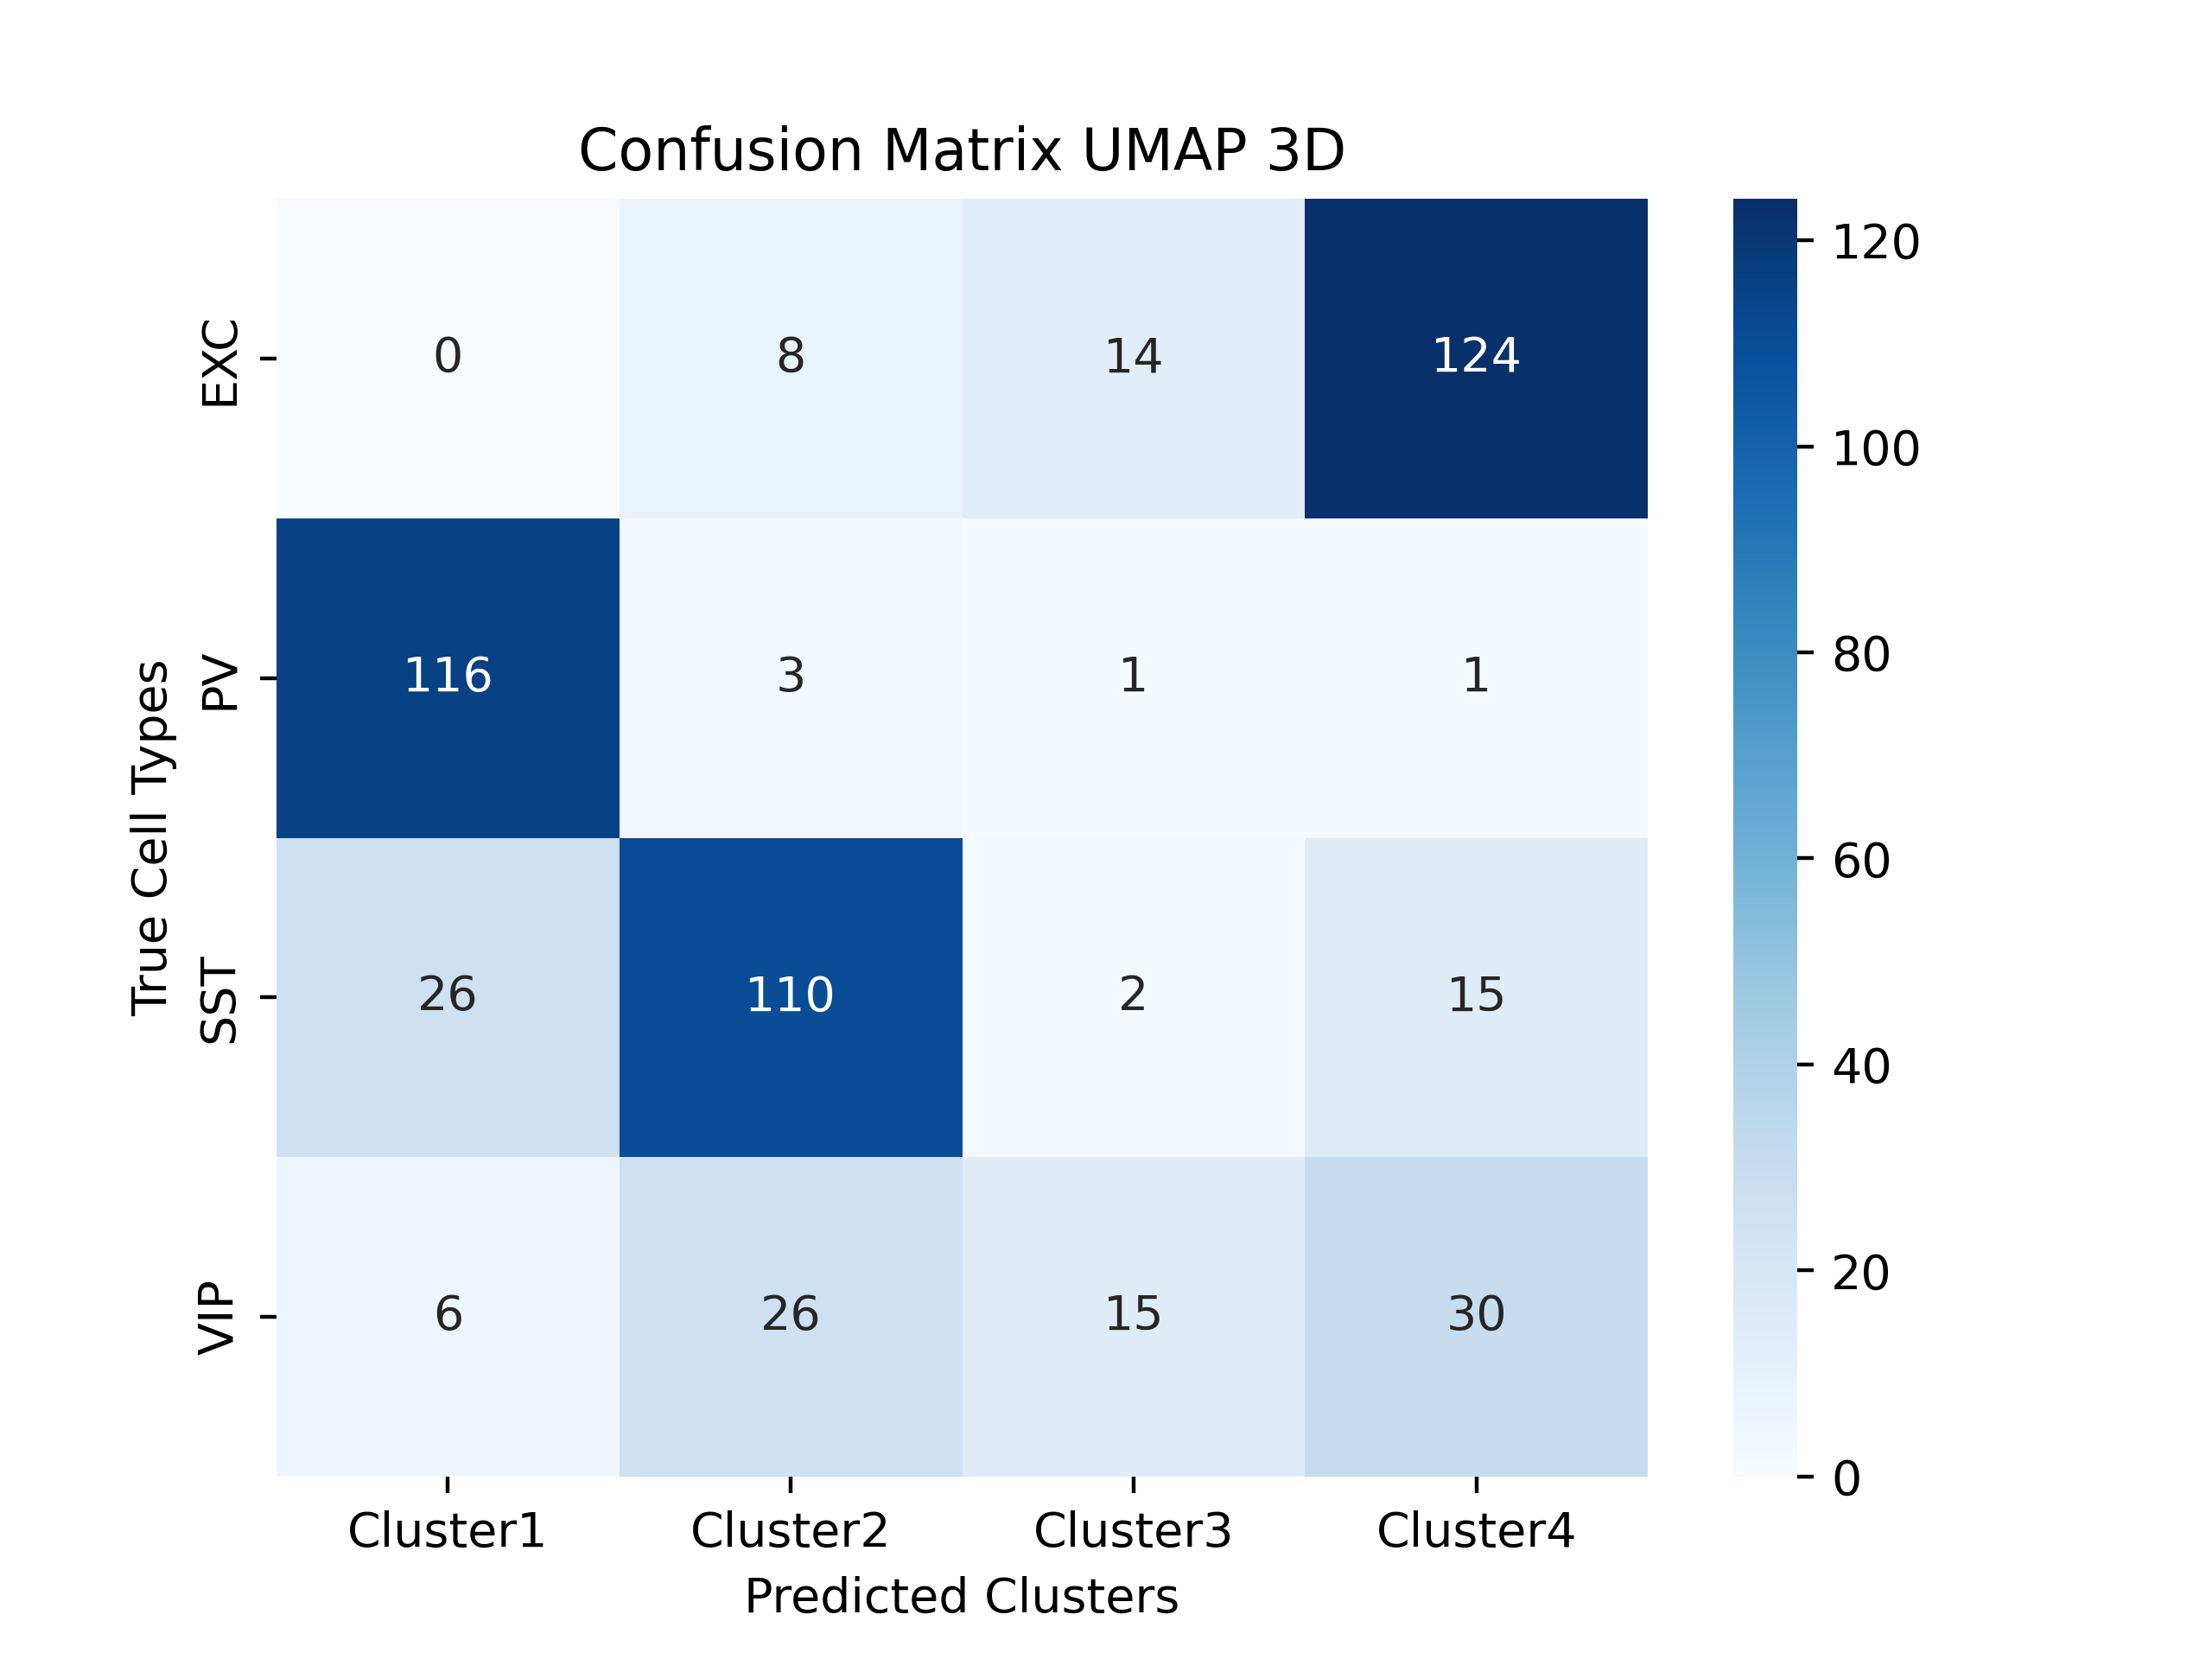
\includegraphics[width=0.45\columnwidth]{figures/Confusion Matrix UMAP 3D.png}
  \caption{K-Means Clustering Confusion Matrices. Top row is PCA. Middle row is t-SNE. Bottom row is UMAP. Left column in 2D. Right column in 3D.}%
  \label{fig:unsupervised_confusion_matrices}
\end{figure}

\begin{figure}[h!]
  \centering
  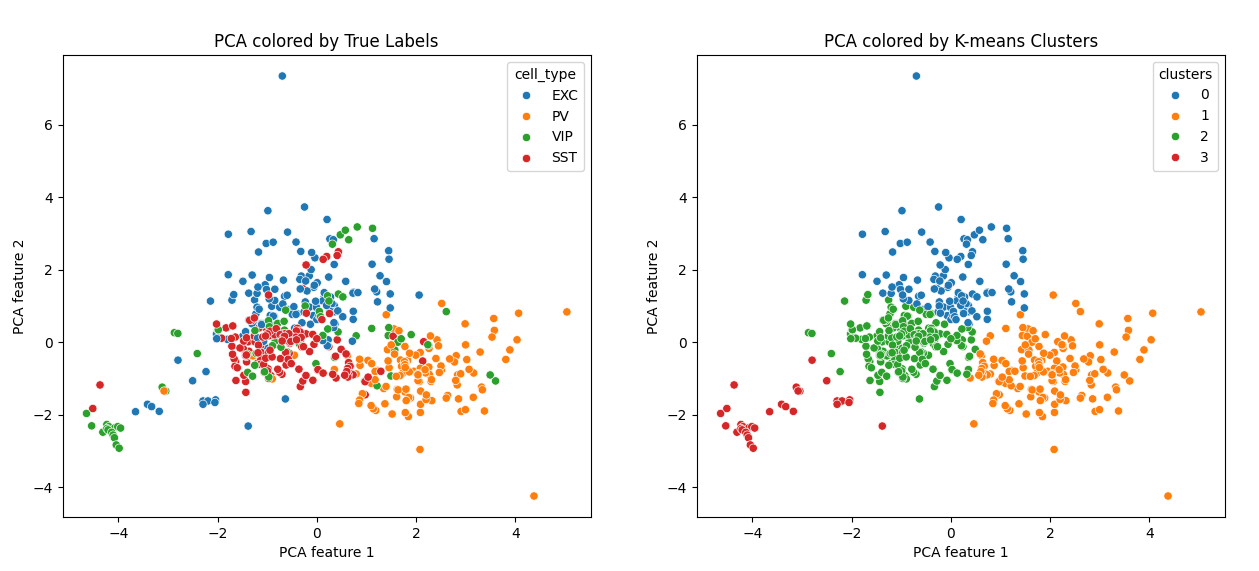
\includegraphics[width=1\columnwidth]{figures/Compare PCA 2D.png}
  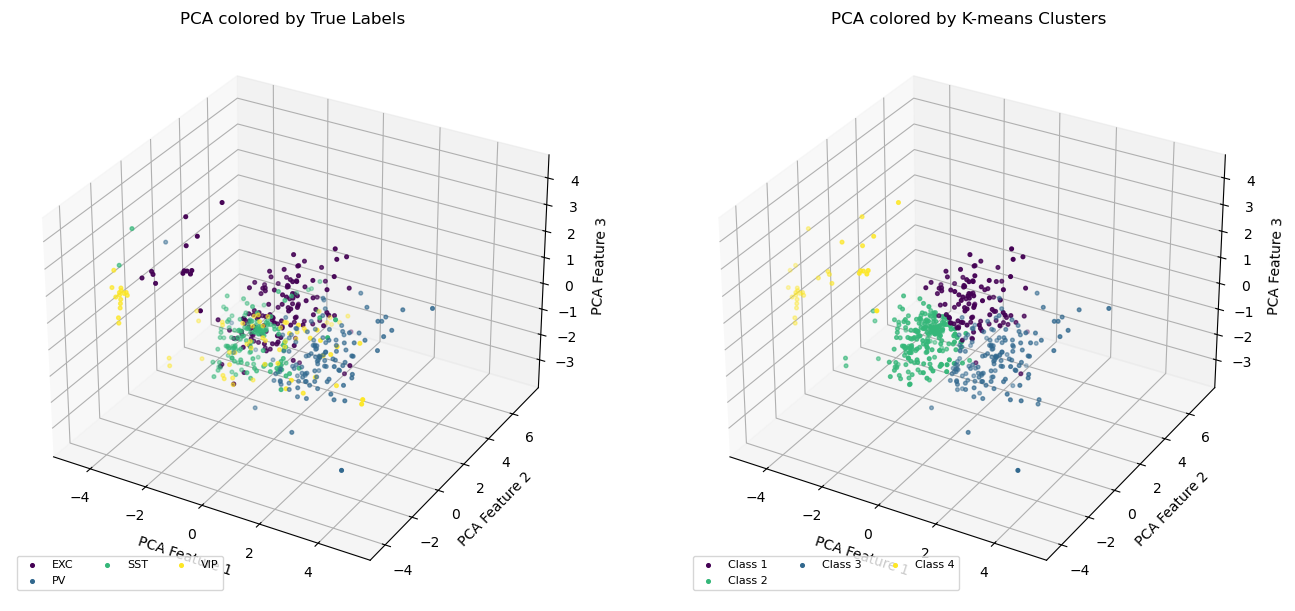
\includegraphics[width=1\columnwidth]{figures/Compare PCA 3D.png}
  \caption{2D (top row) and 3D (bottom row) PCA projections of the data. Left column is colored by true labels, and right column is colored by K-Means clustering.}%
  \label{fig:pca}
\end{figure}

\begin{figure}[h!]
  \centering
  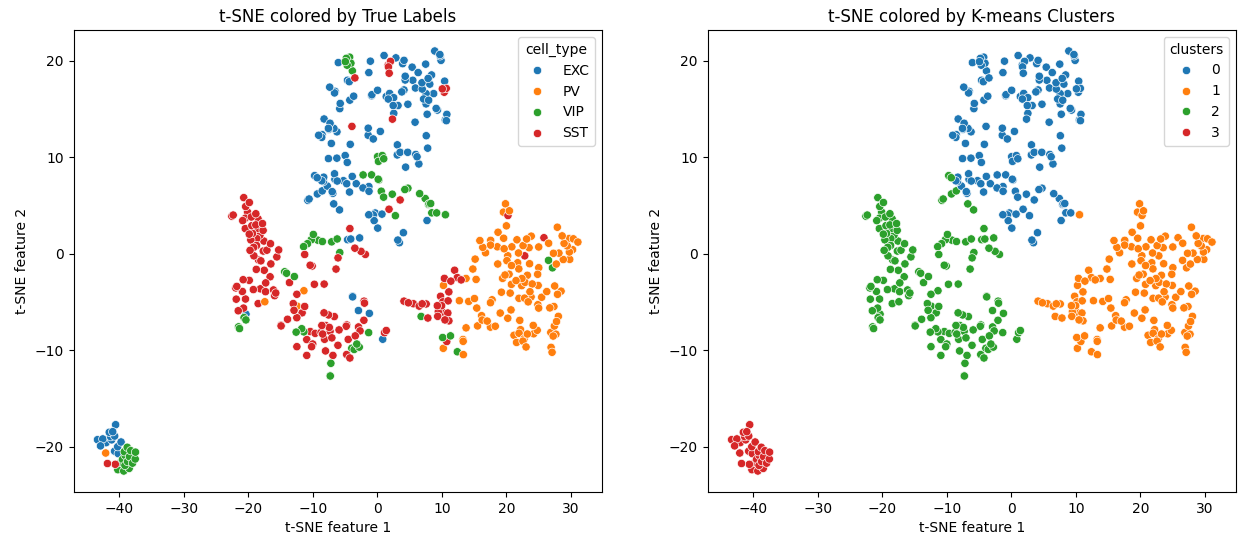
\includegraphics[width=1\columnwidth]{figures/Compare t-SNE 2D.png}
  \includegraphics[width=1\columnwidth]{figures/Compare t-SNE 3D.png}
  \caption{2D (top row) and 3D (bottom row) t-SNE projections of the data. Left column is colored by true labels, and right column is colored by K-Means clustering.}%
  \label{fig:t-SNE}
\end{figure}

From both PCA, t-SNE and UMAP (Fig. \ref{fig:pca}, \ref{fig:t-SNE}, \ref{fig:umap}), there emerges similar patterns in the way cell classes are predisposed. PV cells seem to be more separated, and less mixed with other cell types. VIP cells are scattered and are not captured within a region of space, unlike the other cell classes.
SST and EXC cells are depicted close to each other.
Finally, a small, mixed class, grouping of points is always present in the bottom left corner of 2D projections.

\subsection{Unsupervised Performance}

\begin{figure}[h!]
  \centering
  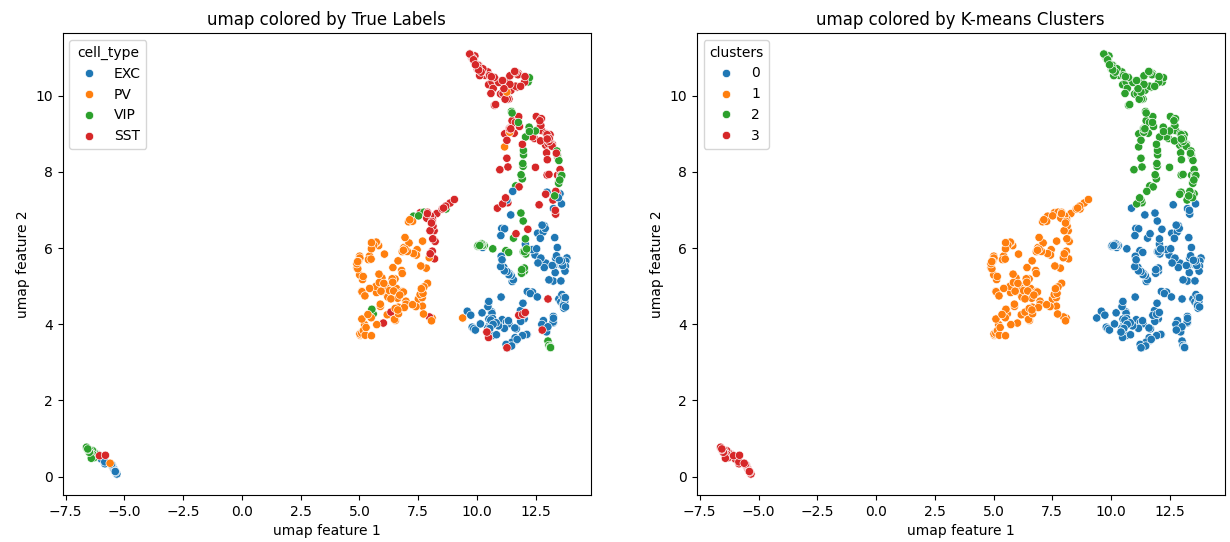
\includegraphics[width=1\columnwidth]{figures/Compare UMAP 2D.png}
  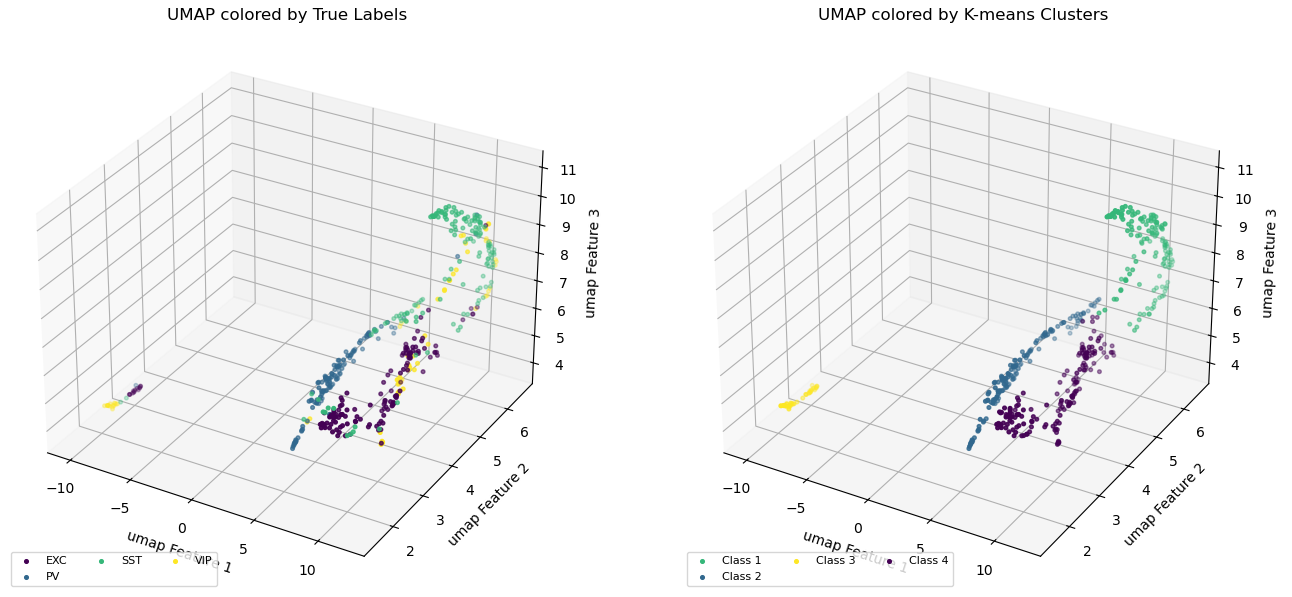
\includegraphics[width=1\columnwidth]{figures/Compare UMAP 3D.png}
  \caption{2D (top row) and 3D (bottom row) UMAP projections of the data. Left column is colored by true labels, and right column is colored by K-Means clustering.}%
  \label{fig:umap}
\end{figure}

K-Means clustering was a majority of times able to attribute a cluster to the region with the highest density of EXC, SST and PV cells (Fig. \ref{fig:pca}, \ref{fig:t-SNE}, \ref{fig:umap}). Due to the presence of the separated mixed grouping in the bottom left corner of each different dimensional space, it is always predicted as the final cluster.
When looking at the confusion matrix from Fig. \ref{fig:unsupervised_confusion_matrices} one can observe the same phenomenon as described above. A cluster is always attributed to PV cells (cluster 2 and 1, for PCA, 1 and 1 for t-SNE, 4 and 1 for UMAP, respectively for 2D and 3D data). Although less pronounced, the same can be said for EXC and SST cells (except for PCA data where EXC cells are more sparse). One cluster captures the small mixed grouping consisting of roughly 14 EXC, 1 PV, 1 SST and 15 VIP cells. Also, VIP cells are found in similar ratios within each cluster.

%-----------------------------------------------------

\section{Discussion}

\subsection{Performance}
It is important to note that for a 4-class classification like this one, a ``chance level" score is $F1_{chance}=0.25$.
In that regard, the four best models achieve above $0.87$ performance and the ensemble method is able to reach a score above $0.9$. This is quite impressive considering the relatively low sample size ($n=497$) and the moderate class imbalance present in our data. This means that there are definitely characteristics that can help to differentiate and discriminate between the different cell classes. Due to this high performance, we can also be more confident in our feature importance analysis.

\subsection{Cell Class Specificity}
Despite the fact that each supervised learning model is built differently, they all agree on certain aspects. It is hard to predict VIP cells but easy to predict PV cells.

This is also supported by unsupervised learning. K-Means was able to recognize PV cells quite accurately by grouping all of them into a cluster, but it did not attribute group VIP cells into a specific cluster.

% The lower dimensional spatial similarity found between EXC and SST cells could highlight the biological action similarity between the two. SST cells can also inhibit other GABAergic neurons, which in turn can lead to an excitation.

The small mixed grouping of points found bottom left of dimensionally reduced spaces (Fig. \ref{fig:pca}, \ref{fig:t-SNE}, \ref{fig:umap}), is probably due to the biologically nonsensical preprocessing step of replacing nonexistent AP durations and thresholds by a value of zero. This could mean that the 14 EXC, 1 PV, 1 SST and 15 VIP cells, mostly present in that grouping would have had no AP in their sweep.

\subsection{General and Cell Specific Important Features}

While being relatively simple, an advantage of linear model becomes clear due to the ease of interpretability.
The important features for each supervised method repeat themselves. They are very similar in between types of models i.e. tree-based methods and linear methods, which is expected. The shared importance of features highlights the robustness of these factors in classifying cell types. This consistency suggests a biological relevance to these features.
AP duration, firing rate and spectral characteristics were already identified as being good discriminants, but new features such as the number of bursts, the downward or upward phase of AP downstroke, influenced by ion channel dynamics in repolarization, seem to vary across EXC, PV, SST and VIP cell types.
This generally reflects the overall balance of excitatory and inhibitory inputs.

%-----------------------------------------------------

\section{Conclusion}

This study has undertaken a comprehensive exploration of machine learning methodologies applied to electrophysiological data. The supervised learning models, ranging from Gradient Boosting to Support Vector Machines, showcase impressive performance in differentiating cell types, with an ensemble model further elevating classification accuracy. Feature importance analyses reveal recurring themes across models, that were previously reported, emphasizing once again the significance of action potential duration, firing rates, and spectral characteristics, but also newly explored features such as the number of bursts or the action potential downstroke. In the realm of unsupervised learning, dimensionality reduction techniques provide insightful visualizations, hinting at spatial arrangements and inter-class relationships. While challenges persist, such as the elusive predictability of VIP cells, the study offers valuable insights into the discriminative features governing neuronal classifications, contributing to the broader understanding of neural dynamics and function.


%-----------------------------------------------------
\newpage
\section{Annex}


\begin{figure}[h!]
  \centering
  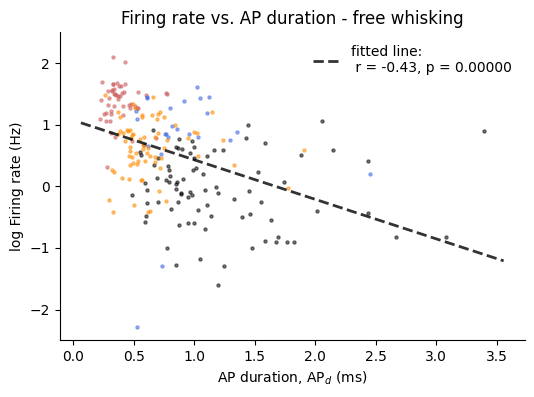
\includegraphics[width=0.45\columnwidth]{figures/given/3_Mean_FRvsAP_Duration.png}
  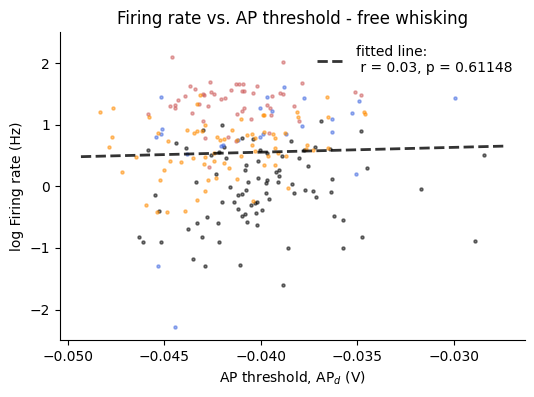
\includegraphics[width=0.45\columnwidth]{figures/given/8_Mean_FR_Correlations_APthreshold.png}
  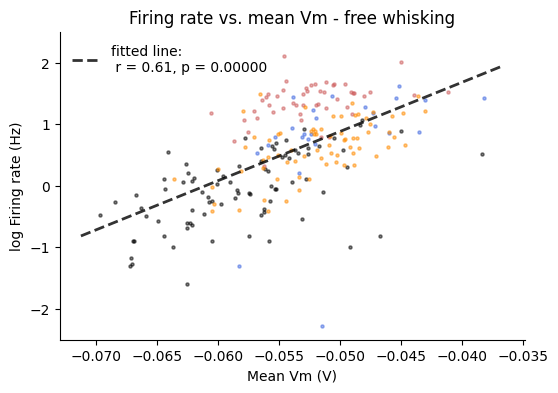
\includegraphics[width=0.45\columnwidth]{figures/given/8_Mean_FR_Correlations_meanVm.png}
  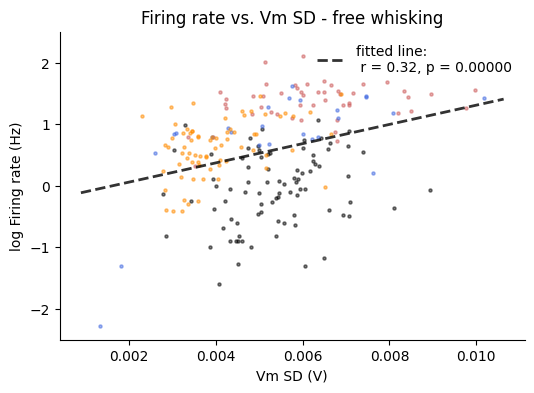
\includegraphics[width=0.45\columnwidth]{figures/given/8_Mean_FR_Correlations_VmSD.png}
  \caption{1. Mean Firing Rate vs. Action Potential Duration. 2. Mean Firing Rate Correlations with Action Potential Threshold. 3. Mean Firing Rate Correlations with Mean Membrane Potential. 4. Mean Firing Rate Correlations with Membrane Potential Standard Deviation.}%
  \label{fig:3_8}
\end{figure}

\begin{figure}[h!]
  \centering
  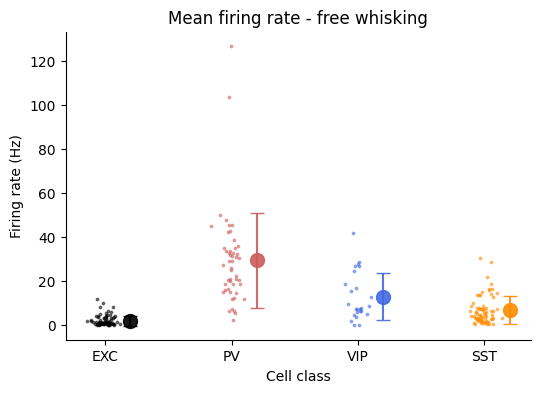
\includegraphics[width=0.3\columnwidth]{figures/given/1_Mean_Firing_Rate.png}
  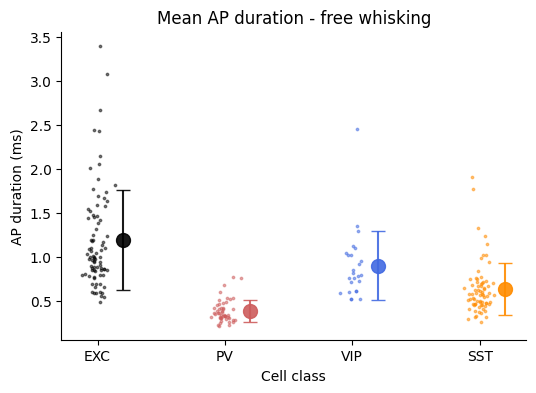
\includegraphics[width=0.3\columnwidth]{figures/given/2_Mean_AP_Duration.png}
  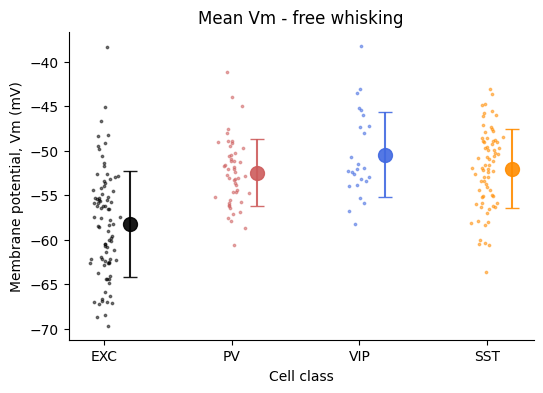
\includegraphics[width=0.3\columnwidth]{figures/given/4_Mean_Vm.png}
  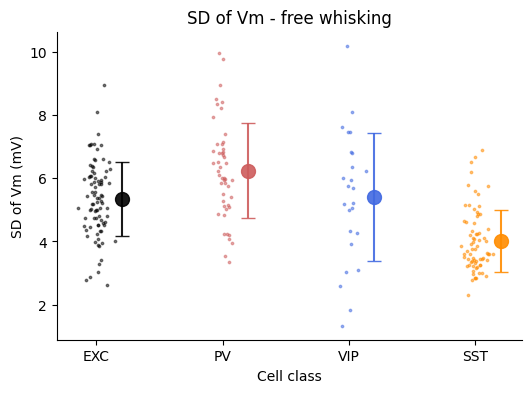
\includegraphics[width=0.3\columnwidth]{figures/given/5_Mean_Vm_SD.png}
  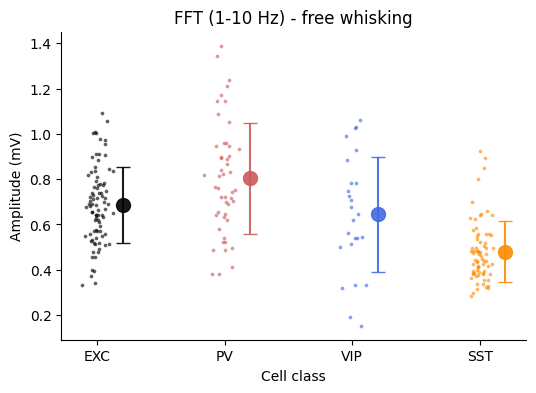
\includegraphics[width=0.3\columnwidth]{figures/given/7_Mean_FFT_LF.png}
  \caption{1. Mean Firing Rate. 2. Mean Action Potential Duration. 3. Mean Membrane Potential. 4. Mean Membrane Potential Standard Deviation. 5. Mean Fourier Transform Low Frequency.}%
  \label{fig:1_2_4_5_7}
\end{figure}

\begin{figure}[h!]
  \centering
  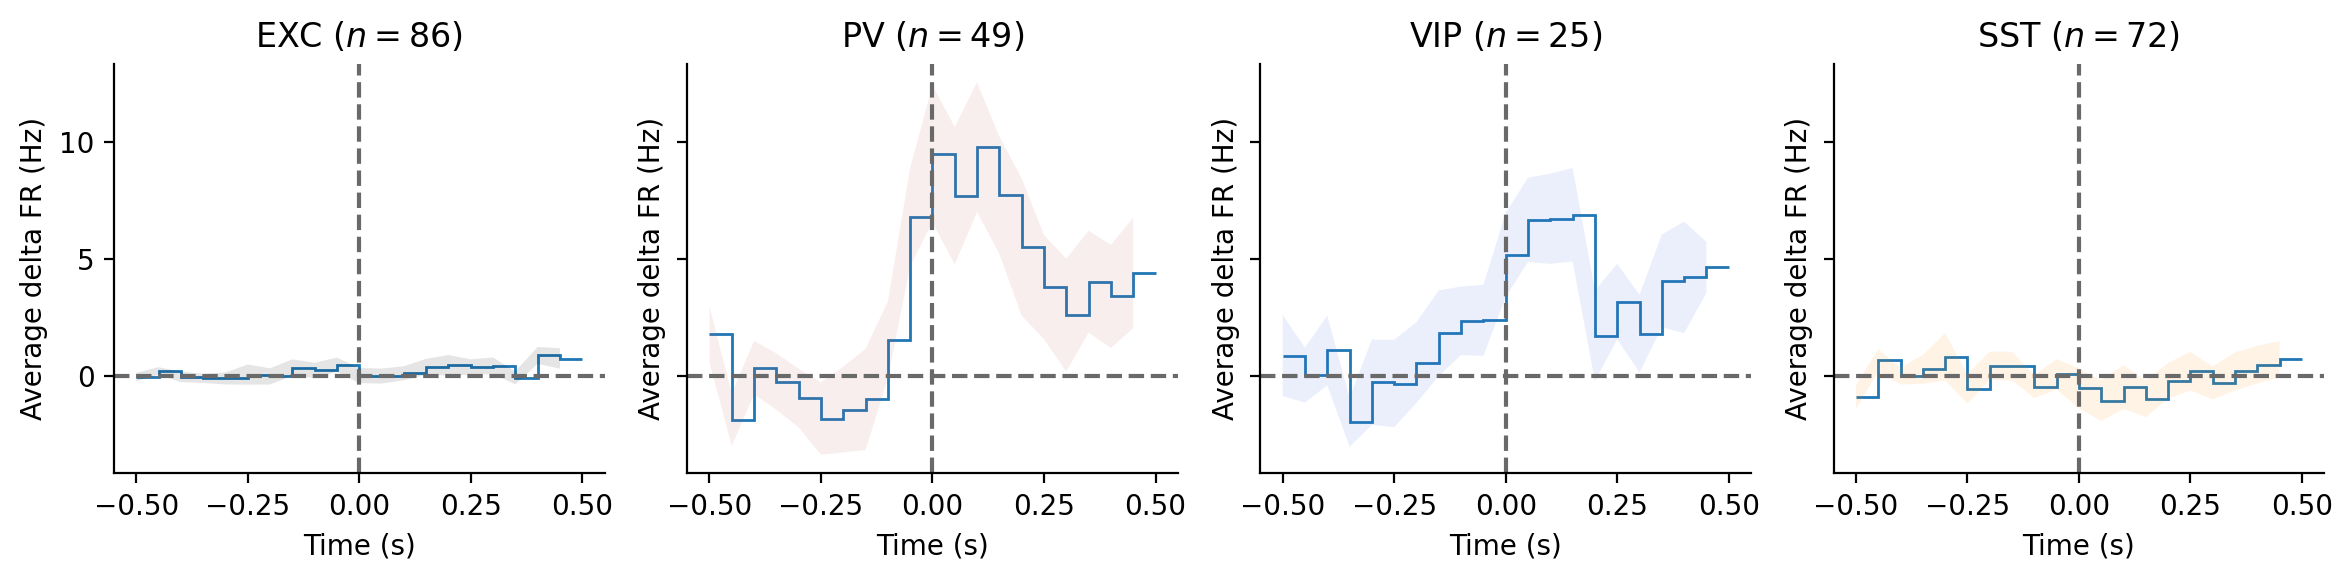
\includegraphics[width=0.9\columnwidth]{figures/given/9_WhiskOnset_GRD_AVG_FirinRate.png}
  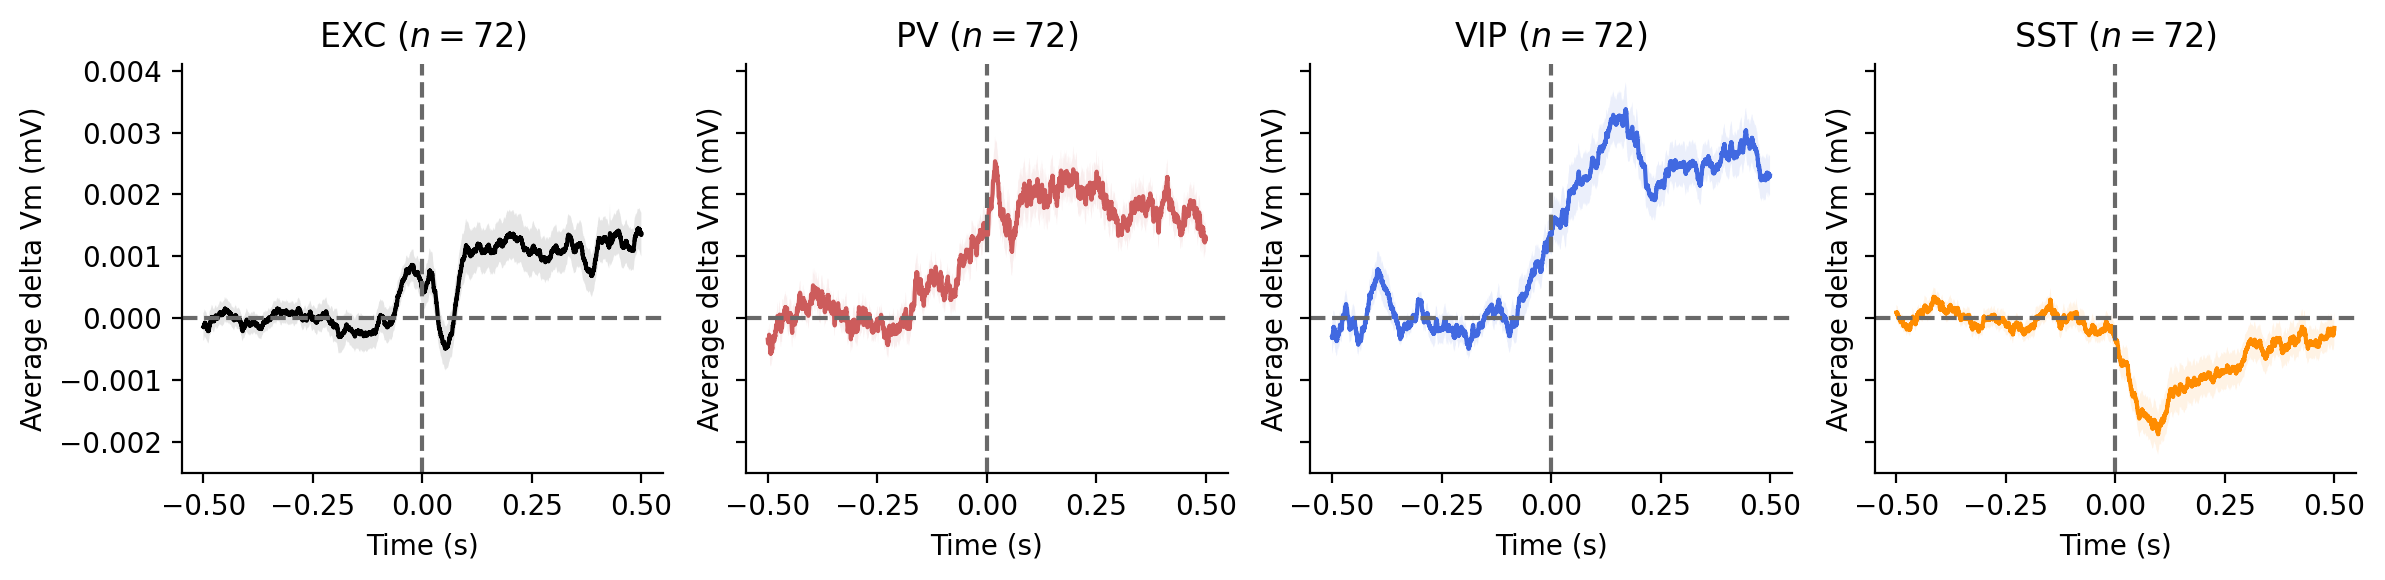
\includegraphics[width=0.9\columnwidth]{figures/given/9_WhiskOnset_GRD_AVG_Vm.png}
  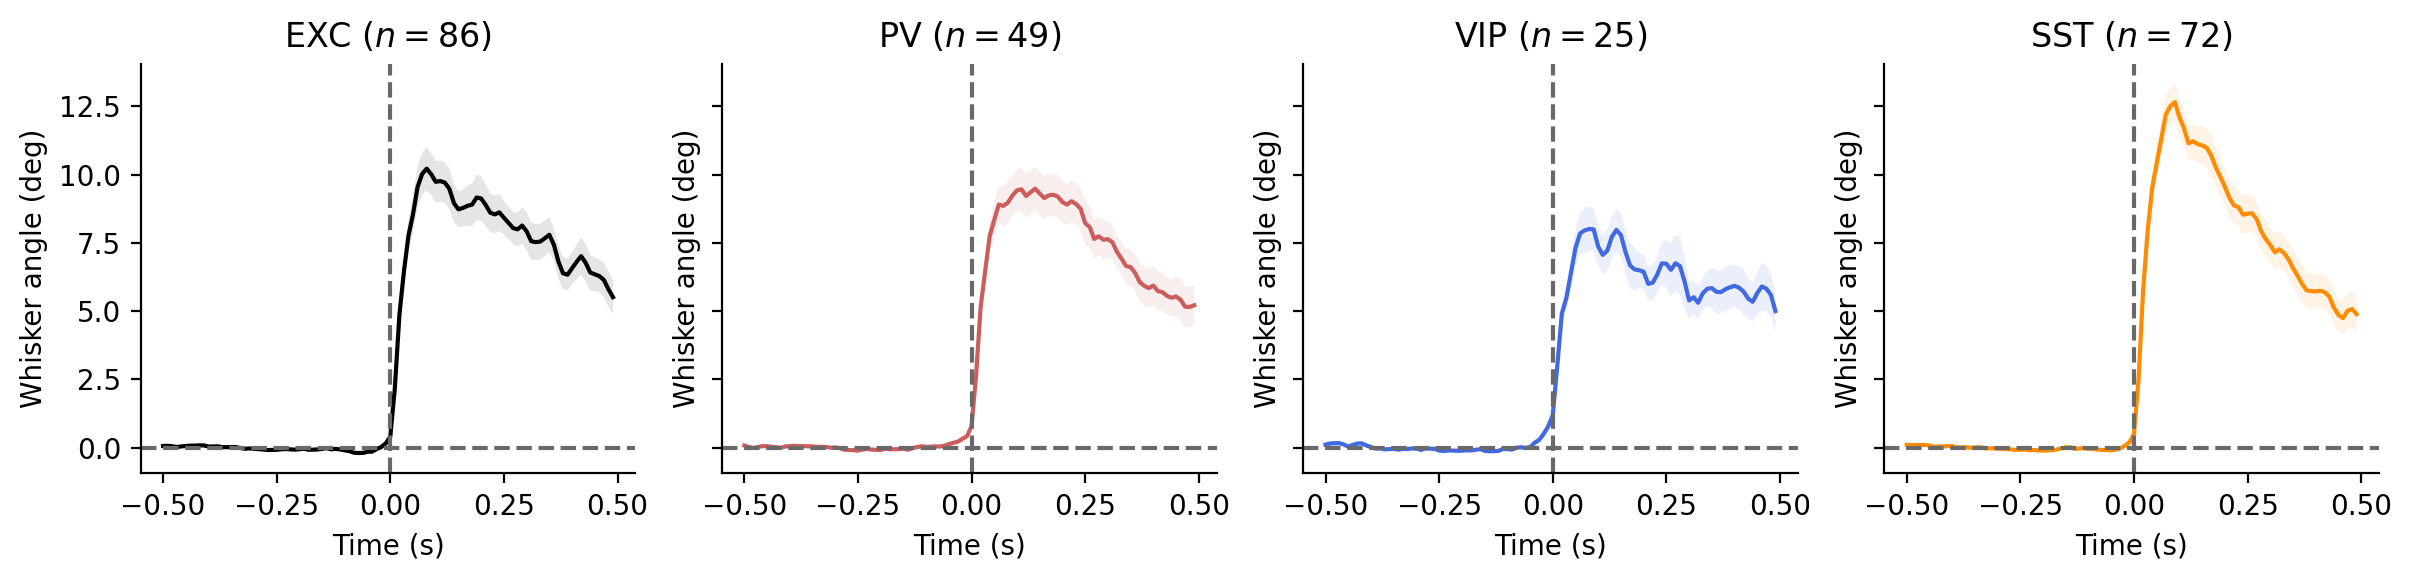
\includegraphics[width=0.9\columnwidth]{figures/given/9_WhiskOnset_GRD_AVG_WhiskerAngle.png}
  \caption{1. Whisker Onset Gradient-Averaged Firing Rate. 2. Whisker Onset Gradient-Averaged Membrane Potential. 3. Whisker Onset Gradient-Averaged Whisker Angle.}%
  \label{fig:9}
\end{figure}

\begin{figure}[h!]
  \centering
  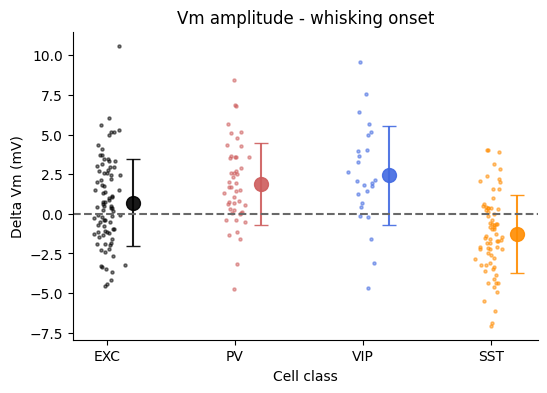
\includegraphics[width=0.45\columnwidth]{figures/given/10_delta_vm_whisking_onset.png}
  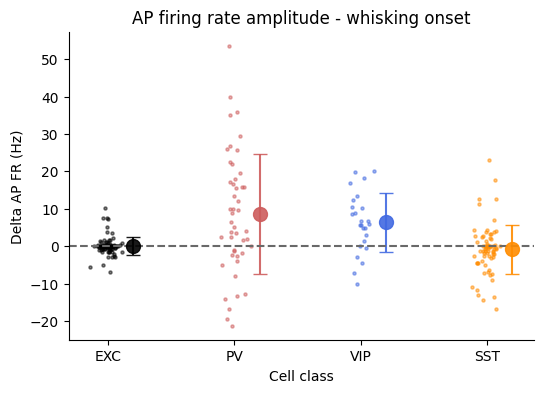
\includegraphics[width=0.45\columnwidth]{figures/given/11_delta_ap_fr_whisking_onset.png}
  \caption{1. Delta Membrane Potential at Whisking Onset. 2. Delta Action Potential Firing Rate at Whisking Onset.}%
  \label{fig:10_11}
\end{figure}

\begin{figure}[h!]
  \centering
  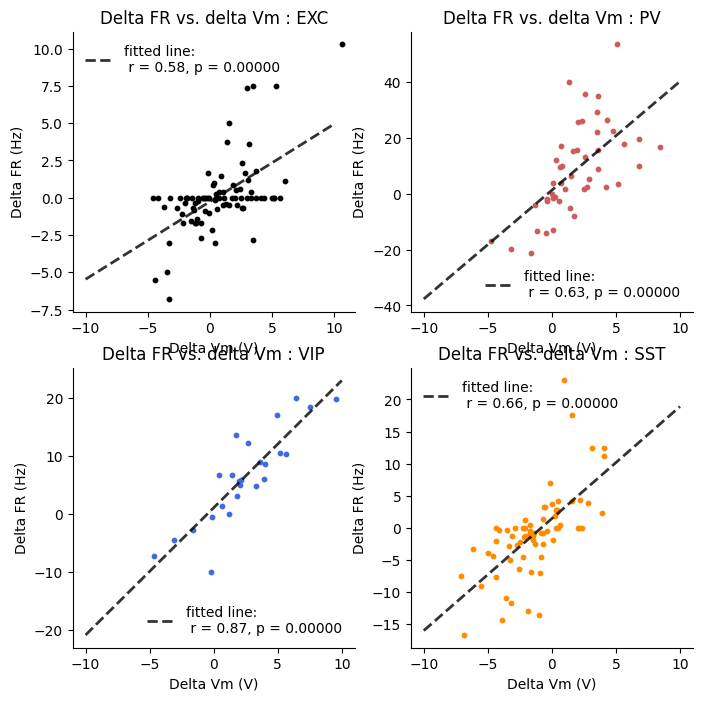
\includegraphics[width=\columnwidth]{figures/given/12_delta_FRvsdelta_Vm.png}
  \caption{Delta Firing Rate vs. Delta Membrane Potential.}%
  \label{fig:12}
\end{figure}

\begin{figure}[h!]
  \centering
  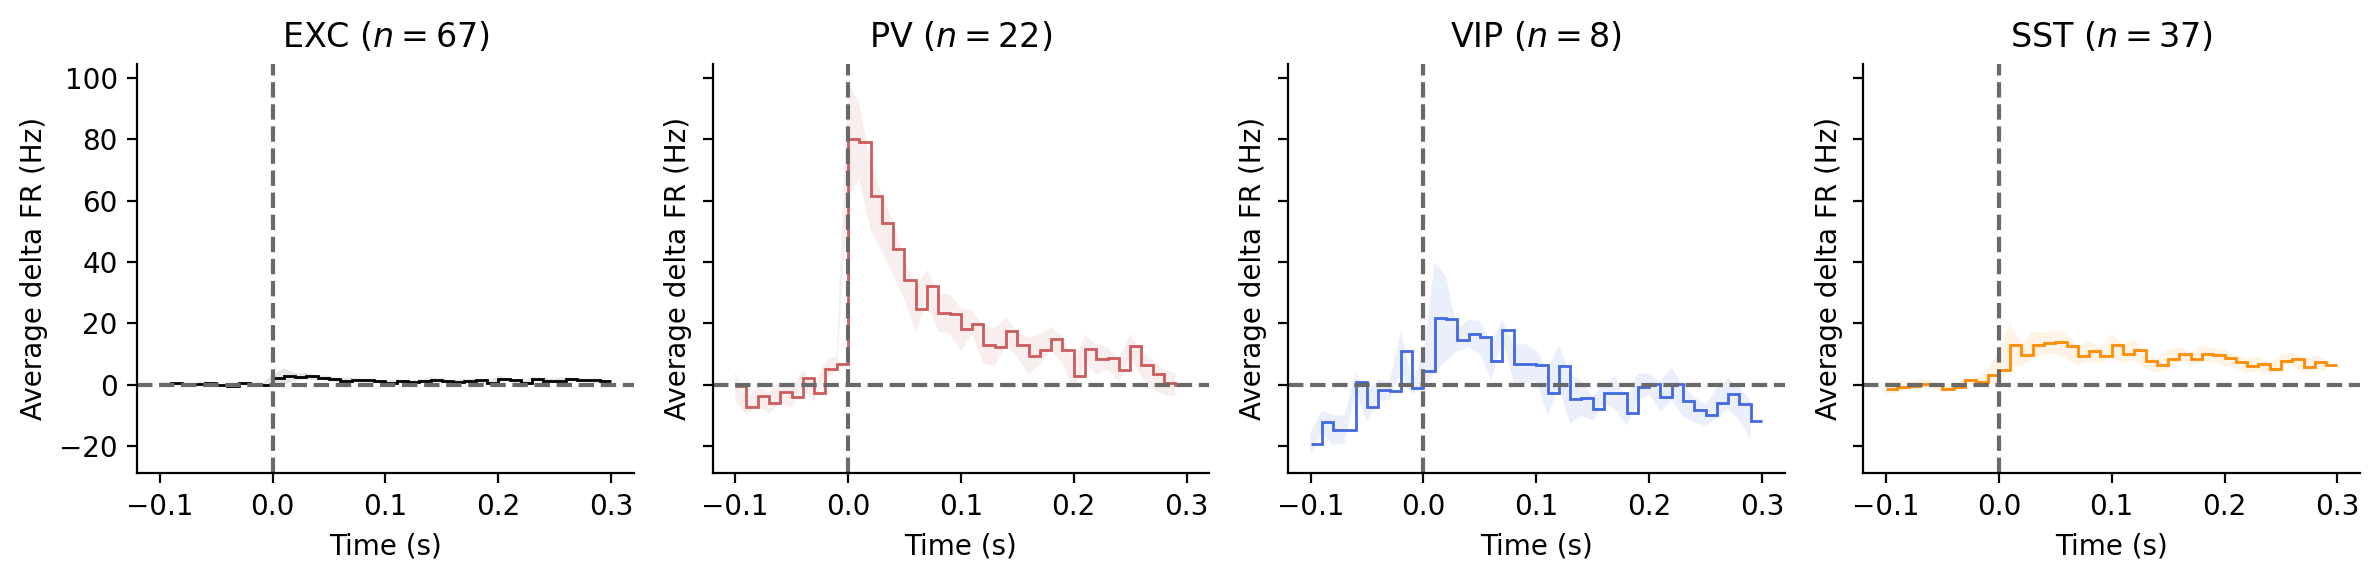
\includegraphics[width=0.9\columnwidth]{figures/given/13_TouchOnset_GRD_AVG_FiringRate.png}
  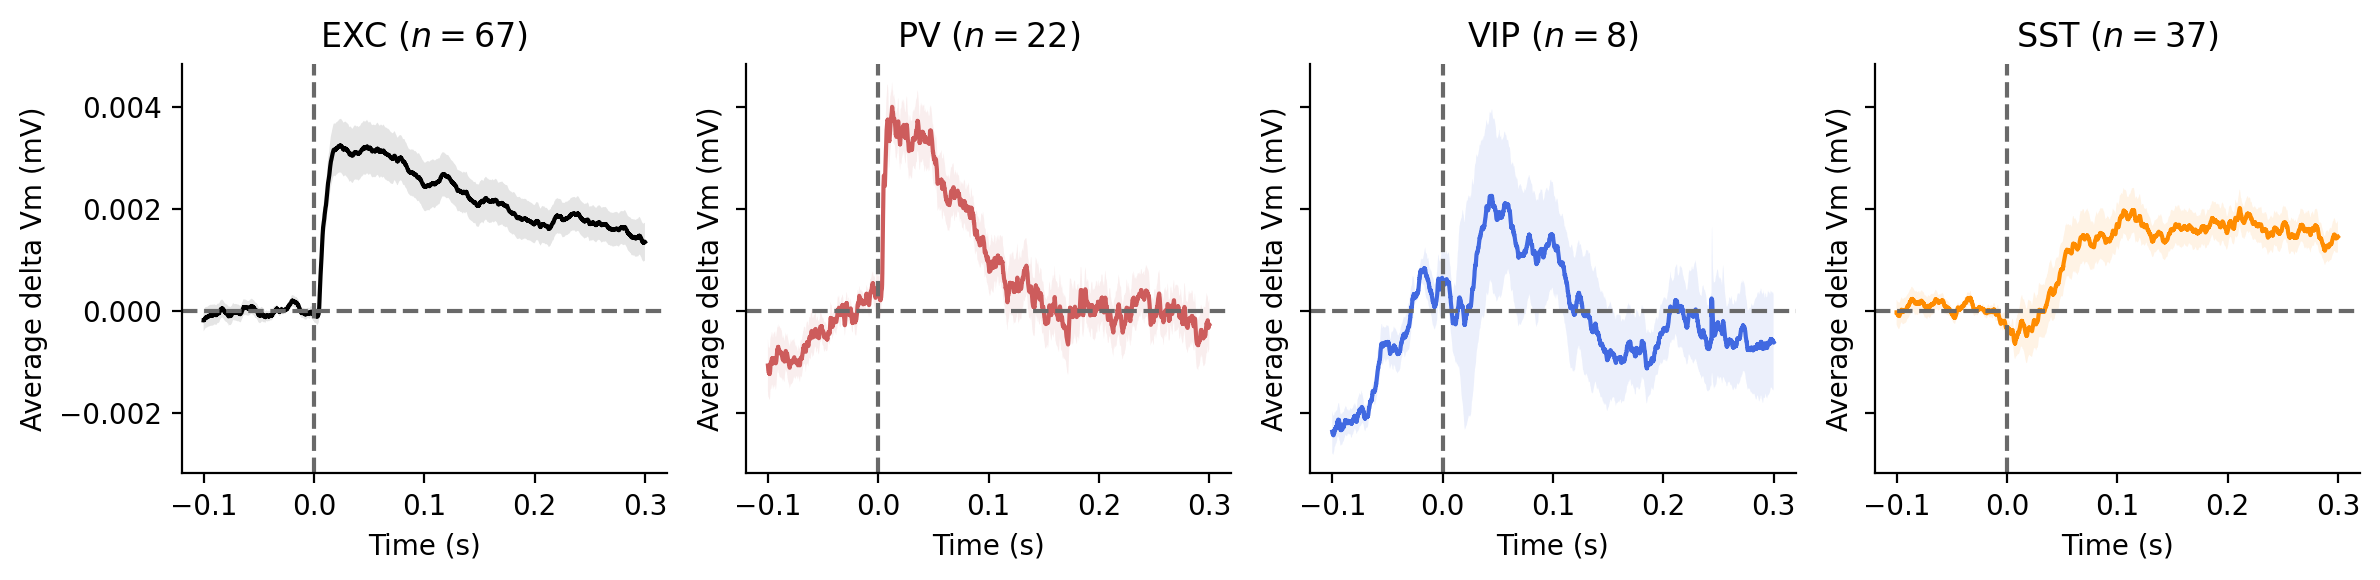
\includegraphics[width=0.9\columnwidth]{figures/given/13_TouchOnset_GRD_AVG_Vm.png}
  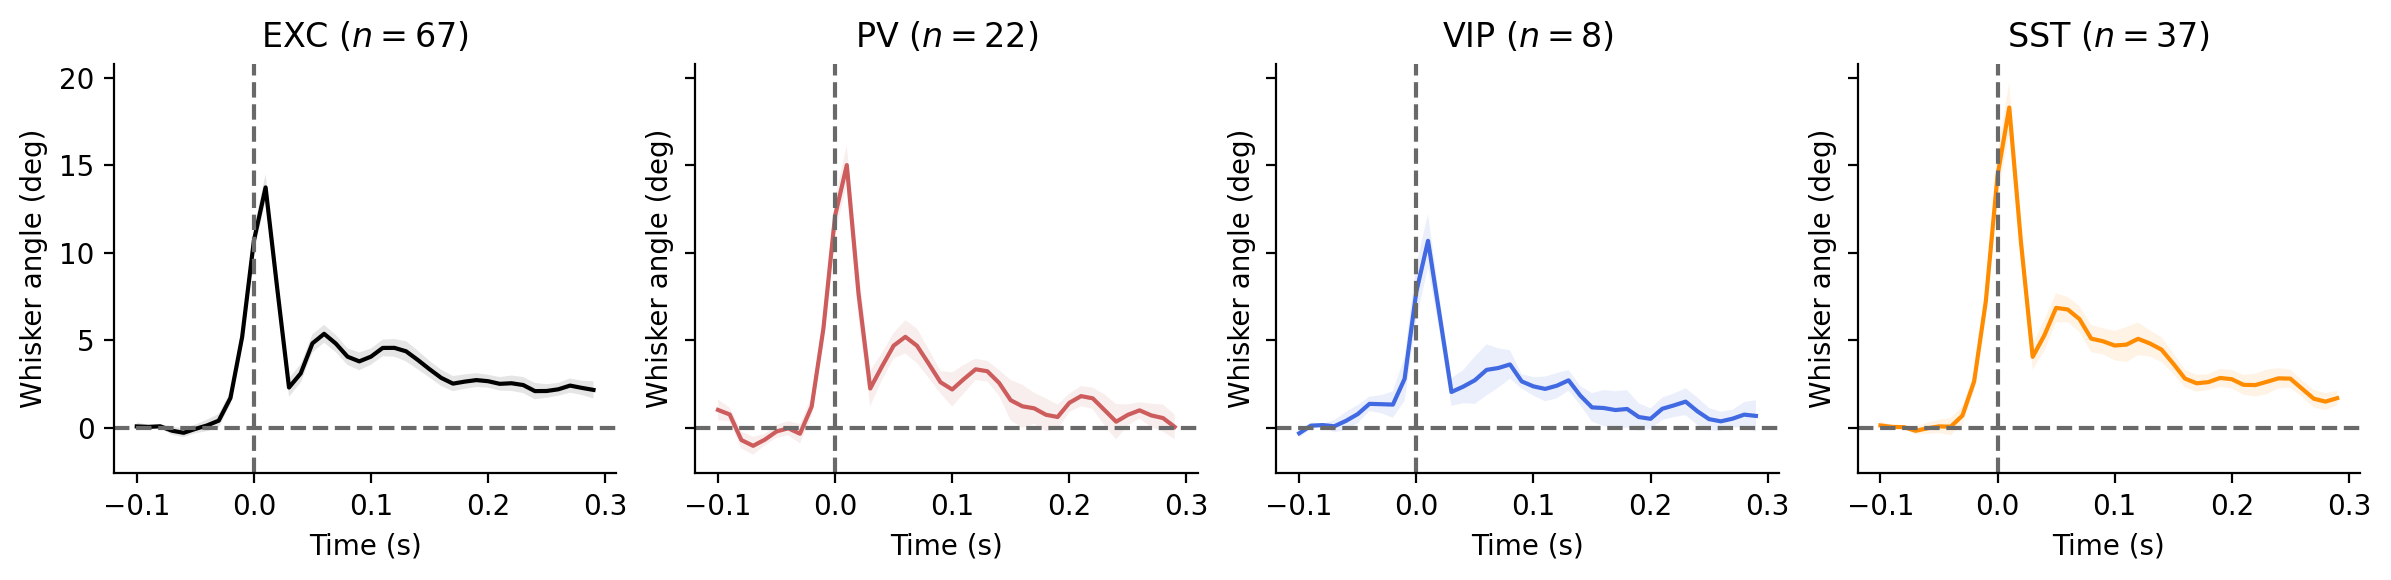
\includegraphics[width=0.9\columnwidth]{figures/given/13_TouchOnset_GRD_AVG_WhiskerAngle.png}
  \caption{1. Touch Onset Gradient-Averaged Firing Rate. 2. Touch Onset Gradient-Averaged Membrane Potential. 3. Touch Onset Gradient-Averaged Whisker Angle.}%
  \label{fig:13}
\end{figure}

\begin{figure}[h!]
  \centering
  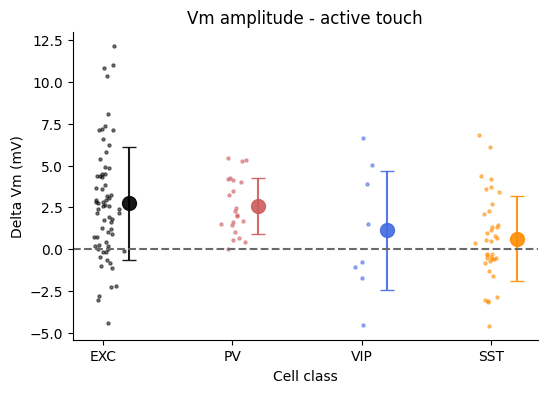
\includegraphics[width=0.45\columnwidth]{figures/given/14_delta_Vm_active_touch.png}
  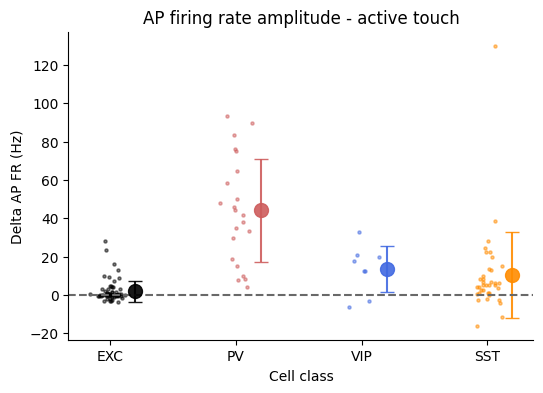
\includegraphics[width=0.45\columnwidth]{figures/given/15_delta_FR_active_touch.png}
  \caption{1. Delta Membrane Potential during Active Touch. 2. Delta Firing Rate during Active Touch.}%
  \label{fig:14_15}
\end{figure}

\begin{figure}[h!]
  \centering
  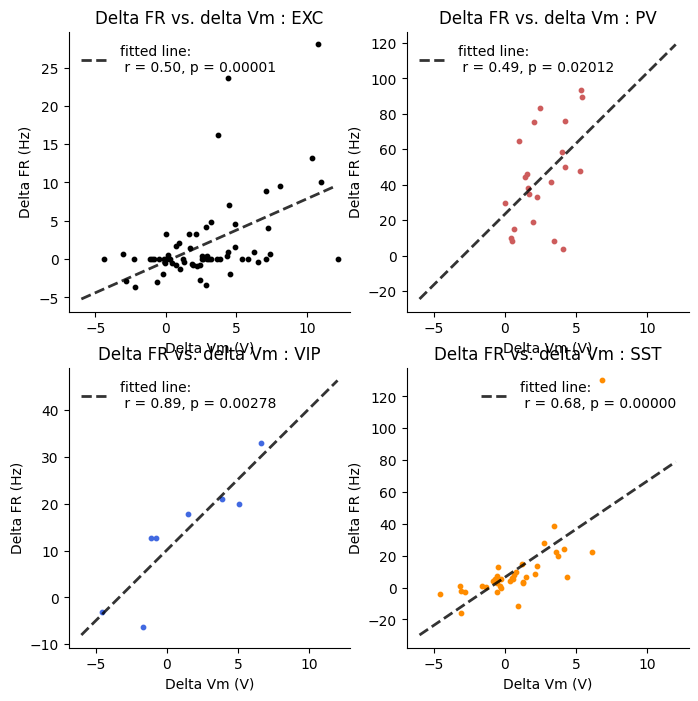
\includegraphics[width=\columnwidth]{figures/given/16_delta_FRvsdelta_Vm.png}
  \caption{Delta Firing Rate vs. Delta Membrane Potential during Active Touch.}%
  \label{fig:16}
\end{figure}

% TODO: Add this two column figure
\begin{figure*}
  \centering
  \includegraphics[width=\textwidth]{figures/correlation_heatmap.png}
  \caption{Correlation of each predictor with one another within the training data}
  \label{fig:correlation}
\end{figure*}


\begin{table}[h!]
  \centering
  \begin{tabular}{|c|c|}
      \hline
      \textbf{Model} & \textbf{Hyperparameters} \\
      \hline
      Gradient Boosting & Learning Rate: 1.0, Max Depth: 2, N Estimators: 176 \\
      \hline
      Linear SVC & C: 0.8428, Multi-class: Crammer-Singer \\
      \hline
      Random Forest & Max Depth: 9, N Estimators: 174, Min Samples Leaf: 1 \\
      \hline
      Logistic Regression & C: 5.241 \\
      \hline
  \end{tabular}
  \caption{Hyperparameters of Different Models. Any parameter not mentioned is equal to the default parameter in Sci-kit Learn.}
  \label{tab:hyperparameters}
\end{table}


\end{document}